% --------------------------------------------------------
% DEFINIÇÕES DO DOCUMENTO
% --------------------------------------------------------

\documentclass[
	% -- opções da classe memoir --
	12pt,				% tamanho da fonte
	openright,			% capítulos começam em pág ímpar (insere página vazia caso preciso)
	oneside,			% para impressão em verso e anverso. Oposto a twoside
	a4paper,			% tamanho do papel.
	% -- opções da classe abntex2 --
	%chapter=TITLE,		% títulos de capítulos convertidos em letras maiúsculas
	%section=TITLE,		% títulos de seções convertidos em letras maiúsculas
	%subsection=TITLE,	% títulos de subseções convertidos em letras maiúsculas
	%subsubsection=TITLE,% títulos de subsubseções convertidos em letras maiúsculas
	% -- opções do pacote babel --
	english,			% idioma adicional para hifenização
	french,				% idioma adicional para hifenização
	spanish,			% idioma adicional para hifenização
	brazil,				% o último idioma é o principal do documento
	]{abntex2}


% --------------------------------------------------------
% PACOTES
% --------------------------------------------------------

\usepackage{cmap}				% Mapear caracteres especiais no PDF
\usepackage{lmodern}			% Usa a fonte Latin Modern
\usepackage[T1]{fontenc}		% Selecao de codigos de fonte.
\usepackage[utf8]{inputenc}		% Codificacao do documento (conversão automática dos acentos)
\usepackage{tabularx} % Pacote para tabelas com largura fixa
\usepackage{lipsum} % Apenas para gerar texto de exemplo
\usepackage{ragged2e} % Para alinhar o texto nas colunas (por ex., justificá-lo)
\usepackage{booktabs} % Para linhas horizontais mais profissionais na tabela
\usepackage{CJKutf8}
\usepackage{lastpage}			% Usado pela Ficha catalográfica
\usepackage{indentfirst}		% Indenta o primeiro parágrafo de cada seção.
\usepackage{color}				% Controle das cores
\usepackage{graphicx}			% Inclusão de gráficos
\usepackage{lipsum}				% para geração de dummy text
\usepackage[brazilian,hyperpageref]{backref}	 % Paginas com as citações na bibl
\usepackage[alf]{abntex2cite}	% Citações padrão ABNT
\usepackage[br]{nicealgo}       % Pacote para criação de algoritmos
\usepackage{customizacoes}      % Pacote de customizações do abntex2
\usepackage{float}
\usepackage{amsmath}
\usepackage{enumitem}
\usepackage{lipsum} % Para texto de exemplo
\usepackage{tabularx} % Pacote para tabelas que se ajustam automaticamente
\usepackage{ragged2e} % Para alinhar o texto à esquerda
\usepackage{booktabs} % Para linhas horizontais mais profissionais
\usepackage[a4paper, margin=2.5cm]{geometry} % Para definir as margens
% --------------------------------------------------------
% CONFIGURAÇÕES DE PACOTES
% --------------------------------------------------------

% Configurações do pacote backref
\renewcommand{\familydefault}{\sfdefault}
\newcommand\textkorean[1]{%
  \begin{CJK}{UTF8}{mj}#1\end{CJK}}
% Usado sem a opção hyperpageref de backref
% \renewcommand{\backrefpagesname}{Citado na(s) página(s):~}
% Texto padrão antes do número das páginas
% \renewcommand{\backref}{}
% Define os textos da citação
% \renewcommand*{\backrefalt}[4]{
% 	\ifcase #1 %
% 		Nenhuma citação no texto.%
% 	\or
% 		Citado na página #2.%
% 	\else
% 		Citado #1 vezes nas páginas #2.%
% 	\fi}%


% --------------------------------------------------------
% INFORMAÇÕES DE DADOS PARA CAPA E FOLHA DE ROSTO
% --------------------------------------------------------

\titulo{Fed-IDS Privado: Auditoria e Mitigação de Membership Inference em Aprendizado Federado para Detecção de Intrusões}
\autor{Ana Caroline Silva Pontara}
\local{Bauru}
\data{2026}
\orientador{Prof. PhD. Kelton Augusto Pontara da Costa}
\instituicao{%
  Universidade Estadual Paulista ``Júlio de Mesquita Filho''
  \par
  Instituto de Biociências, Letras e Ciências Exatas
  \par
  Programa de Pós-Graduação em Ciência da Computação}
\tipotrabalho{Dissertação (Mestrado)}
\preambulo{Dissertação apresentada ao Programa de Pós-Graduação em Ciência da Computação da Universidade Estadual Paulista ``Júlio de Mesquita Filho'', Instituto de Biociências, Letras e Ciências Exatas, Campus Bauru, como requisito parcial para a obtenção do título de Mestre em Ciência da Computação.}


% --------------------------------------------------------
% CONFIGURAÇÕES PARA O PDF FINAL
% --------------------------------------------------------

% alterando o aspecto da cor azul
\definecolor{blue}{RGB}{41,5,195}

% informações do PDF
\makeatletter
\hypersetup{
     	%pagebackref=true,
		pdftitle={\@title},
		pdfauthor={\@author},
    	pdfsubject={\imprimirpreambulo},
	    pdfcreator={LaTeX with abnTeX2},
		pdfkeywords={abnt}{latex}{abntex}{abntex2}{trabalho acadêmico},
		colorlinks=true,       		% false: boxed links; true: colored links
    	linkcolor=blue,          	% color of internal links
    	citecolor=blue,        		% color of links to bibliography
    	filecolor=magenta,      		% color of file links
		urlcolor=blue,
		bookmarksdepth=4
}
\makeatother


% --------------------------------------------------------
% ESPAÇAMENTOS ENTRE LINHAS E PARÁGRAFOS
% --------------------------------------------------------

% O tamanho do parágrafo é dado por:
\setlength{\parindent}{1.3cm}

% Controle do espaçamento entre um parágrafo e outro:
\setlength{\parskip}{0.2cm}


% --------------------------------------------------------
% COMPILANDO O ÍNDICE
% --------------------------------------------------------

\makeindex


% --------------------------------------------------------
% INÍCIO DO DOCUMENTO
% --------------------------------------------------------

\begin{document}

% Seleciona o idioma do documento (conforme pacotes do babel)
\selectlanguage{brazil}

% Retira espaço extra obsoleto entre as frases.
\frenchspacing


% --------------------------------------------------------
% ELEMENTOS PRÉ-TEXTUAIS
% --------------------------------------------------------

% Capa
\imprimircapa

% Folha de rosto
% (o * indica que haverá a ficha bibliográfica)
\imprimirfolhaderosto*

% Inserir a ficha bibliografica
%\begin{fichacatalografica}
%	\sffamily
%	\vspace*{\fill}					% Posição vertical
%	\begin{center}					% Minipage Centralizado
%	\fbox{\begin{minipage}[c][8cm]{15.5cm}		% Largura
%	\small
%	\imprimirautor
%	\hspace{0.5cm} \imprimirtitulo  / \imprimirautor. --
%	\imprimirlocal, \imprimirdata-
%	\hspace{0.5cm} \pageref{LastPage} p. : il. (algumas color.) ; 30 cm.\\
%	\hspace{0.5cm} \imprimirorientadorRotulo~\imprimirorientador\\
%	\hspace{0.5cm}
%	\parbox[t]{\textwidth}{\imprimirtipotrabalho~--~\imprimirinstituicao,
%	\imprimirdata.}\\
%	\hspace{0.5cm}
%		1. Tags
%		2. Para
%		3. A
%		4. Ficha
%		5. Catalográfica
%	\end{minipage}}
%	\end{center}
%\end{fichacatalografica}

% Inserir folha de aprovação
%\begin{folhadeaprovacao}
%  \begin{center}
%    {\ABNTEXchapterfont\large\imprimirautor}
%    \vspace*{\fill}\vspace*{\fill}
%    \begin{center}
%      \ABNTEXchapterfont\bfseries\Large\imprimirtitulo
%    \end{center}
%    \vspace*{\fill}
%    \hspace{.45\textwidth}
%    \begin{minipage}{.5\textwidth}
%        \imprimirpreambulo
%    \end{minipage}%
%    \vspace*{\fill}
%   \end{center}
%   \center Banca Examinadora
%   \assinatura{\textbf{\imprimirorientador} \\ Orientador}
%   \assinatura{\textbf{Prof. Dr. José Remo Ferreira Brega} \\ Convidado 1}
%   \assinatura{\textbf{Prof. Adj. Roberta Spolon} \\ Convidado 2}
%   \begin{center}
%    \vspace*{0.5cm}
%    \par
%    {São José do Rio Preto, \_\_\_\_\_ de \_\_\_\_\_\_\_\_\_\_\_ de \_\_\_\_.}
%    \vspace*{1cm}
%  \end{center}
%\end{folhadeaprovacao}

% Dedicatória
%\begin{dedicatoria}
%   \vspace*{\fill}
%   \centering
%   \noindent
%   \textit{Espaço destinado à dedicátoria do texto.} \vspace*{\fill}
%\end{dedicatoria}

% Agradecimentos
%\begin{agradecimentos}
%Espaço destinado aos agradecimentos.
%\end{agradecimentos}

% Epígrafe
%\begin{epigrafe}
%    \vspace*{\fill}
%	\begin{flushright}
%		\textit{Espaço destinado à epígrafe.}
%	\end{flushright}
%\end{epigrafe}


% --------------------------------------------------------
% RESUMOS
% --------------------------------------------------------

% resumo em português
% resumo em português
\setlength{\absparsep}{18pt} % ajusta o espaçamento dos parágrafos do resumo
\begin{resumo}
O Aprendizado Federado (FL) emergiu como um paradigma essencial para a construção de Sistemas de Detecção de Intrusão (IDS) colaborativos, ao permitir o treinamento de modelos sem a centralização de dados sensíveis. Contudo, a premissa de privacidade do FL é desafiada por Ataques de Inferência de Pertencimento (\textit{Membership Inference Attacks}, MIA), que podem expor se um registro de dados específico participou do treinamento, revelando informações confidenciais sobre a postura de segurança das organizações. Esta dissertação aborda essa vulnerabilidade crítica, propondo uma metodologia sistemática para a auditoria e mitigação de MIA em IDS Federados (Fed-IDS). O trabalho investiga a aplicação de defesas híbridas, que articulam mecanismos como Privacidade Diferencial (DP-SGD), regularização de modelo e compressão de gradientes, para proteger os modelos contra ataques de inferência. A contribuição central reside na avaliação empírica e quantitativa do \textit{trade-off} entre a utilidade do modelo sua capacidade de detectar intrusões com precisão e o nível de privacidade alcançado pelas defesas. Os resultados demonstram que, embora as defesas mitiguem eficazmente os riscos, elas impõem custos variáveis na performance do IDS, destacando a necessidade de uma calibração cuidadosa para alcançar um equilíbrio ótimo. A pesquisa, portanto, contribui para o desenvolvimento de sistemas de segurança inteligentes que não são apenas eficazes, mas também robustos e genuinamente privados por construção.

\textbf{Palavras-chave:} Aprendizado Federado. Detecção de Intrusão. Inferência de Pertencimento. Privacidade Diferencial. Segurança Cibernética. Fed-IDS.
\end{resumo}

% resumo em inglês
\begin{resumo}[Abstract]
 \begin{otherlanguage*}{english}
Federated Learning (FL) has emerged as an essential paradigm for building collaborative Intrusion Detection Systems (IDS) by enabling model training without centralizing sensitive data. However, the privacy premise of FL is challenged by Membership Inference Attacks (MIA), which can expose whether a specific data record was used in training, revealing confidential information about an organization's security posture. This dissertation addresses this critical vulnerability by proposing a systematic methodology for the audit and mitigation of MIA in Federated IDS (Fed-IDS). The research investigates the application of hybrid defenses, which combine mechanisms such as Differential Privacy (DP-SGD), model regularization, and gradient compression, to protect models against inference attacks. The core contribution lies in the empirical and quantitative evaluation of the trade-off between the model's utility its ability to accurately detect intrusions and the level of privacy achieved by these defenses. The results demonstrate that while the defenses effectively mitigate risks, they impose varying costs on the IDS performance, highlighting the need for careful calibration to achieve an optimal balance. This research, therefore, contributes to the development of intelligent security systems that are not only effective but also robust and genuinely private by design.

\textbf{Keywords:} Federated Learning. Intrusion Detection. Membership Inference. Differential Privacy. Cybersecurity. Fed-IDS.
 \end{otherlanguage*}
\end{resumo}


% --------------------------------------------------------
% LISTA DE ILUSTRAÇÕES
% --------------------------------------------------------

% inserir lista de ilustrações
\pdfbookmark[0]{\listfigurename}{lof}
\listoffigures*
\cleardoublepage


% --------------------------------------------------------
% LISTA DE TABELAS
% --------------------------------------------------------

% inserir lista de tabelas
\pdfbookmark[0]{\listtablename}{lot}
\listoftables*
\cleardoublepage


% --------------------------------------------------------
% LISTA DE ABREVIATURAS E SIGLAS
% --------------------------------------------------------

% inserir lista de abreviaturas e siglas
% Inserir lista de abreviaturas e siglas
\begin{siglas}
  \item[AI] \textit{Artificial Intelligence}
  \item[AUC] \textit{Area Under the Curve}
  \item[AUC-ROC] \textit{Area Under the Receiver Operating Characteristic Curve}
  \item[DP] \textit{Differential Privacy}
  \item[DP-SGD] \textit{Differentially Private Stochastic Gradient Descent}
  \item[FL] \textit{Federated Learning}
  \item[FedAvg] \textit{Federated Averaging}
  \item[FedProx] \textit{Federated Proximal}
  \item[SCAFFOLD] \textit{Stochastic Controlled Averaging for Federated Learning}
  \item[FedOpt] \textit{Federated Optimization}
  \item[Fed-IDS] \textit{Federated Intrusion Detection System}
  \item[FPR] \textit{False Positive Rate}
  \item[IDS] \textit{Intrusion Detection System}
  \item[IoT] \textit{Internet of Things}
  \item[LiRA] \textit{Likelihood Ratio Attack}
  \item[MIA] \textit{Membership Inference Attack}
  \item[ML] \textit{Machine Learning}
  \item[MLaaS] \textit{Machine Learning as a Service}
  \item[Non-IID] \textit{Non-Independent and Identically Distributed}
  \item[ROC] \textit{Receiver Operating Characteristic}
  \item[TPR] \textit{True Positive Rate}
  \item[USENIX] \textit{Advanced Computing Systems Association (United States)}
\end{siglas}


% --------------------------------------------------------
% LISTA DE SÍMBOLOS
% --------------------------------------------------------

% inserir lista de símbolos
%\begin{simbolos}
%  \item[$ \Gamma $] Letra grega Gama
%  \item[$ \Lambda $] Lambda
%  \item[$ \zeta $] Letra grega minúscula zeta
%  \item[$ \in $] Pertence
%\end{simbolos}


% --------------------------------------------------------
% SUMÁRIO
% --------------------------------------------------------

% inserir o sumario
\pdfbookmark[0]{\contentsname}{toc}
\tableofcontents*
\cleardoublepage


% --------------------------------------------------------
% ELEMENTOS TEXTUAIS
% --------------------------------------------------------

\pagestyle{simple}

% Arquivos .tex do texto, podendo ser escritos em um único arquivo ou divididos da forma desejada
\chapter{Introdução}
\label{chap:introducao}

A aplicação de Aprendizado de Máquina na segurança cibernética representa um campo de notável dinamismo, especialmente no desenvolvimento de Sistemas de Detecção de Intrusão. No entanto, esta evolução tecnológica é marcada por uma tensão fundamental: a eficácia dos modelos de ML é diretamente proporcional ao volume e à diversidade dos dados de treinamento, enquanto a natureza sensível dos dados de tráfego de rede impõe restrições severas de privacidade e confidencialidade. O paradigma de treinamento centralizado, embora computacionalmente conveniente, agrava esta tensão ao exigir a consolidação de dados em um repositório único, criando um vetor de ataque de alto valor e um ponto singular de falha.

O Aprendizado Federado emergiu como a resposta arquitetônica mais promissora a esse dilema~\cite{mcmahan2017fedavg}. Ao postular um modelo de treinamento colaborativo sobre dados que permanecem distribuídos e sob o controle local de seus proprietários, o FL propõe uma reconciliação entre a inteligência coletiva e a soberania dos dados. Essa abordagem, que forma a base para a nova geração de IDS Federados (Fed-IDS), representa uma mudança de paradigma ao conciliar a utilidade do modelo com a soberania dos dados locais~\cite{hernandez2023surveyfedids}. No entanto, a garantia de privacidade oferecida pelo FL não é absoluta. Pesquisas recentes demonstraram que a troca de parâmetros do modelo, embora mais segura que a troca de dados, ainda constitui um canal de vazamento de informação~\cite{nasr2019comprehensive}. Adversários podem explorar esses artefatos de aprendizado para executar Ataques de Inferência de Pertencimento (\textit{Membership Inference Attacks}, MIA), cujo objetivo é determinar se um registro de dados específico de um cliente participou do processo de treinamento~\cite{shokri2017mia}. Um ataque bem-sucedido em um Fed-IDS poderia, por exemplo, revelar que o tráfego de rede de uma organização específica continha um padrão de ataque raro, expondo uma vulnerabilidade ou um incidente de segurança que deveria permanecer confidencial.

Essa ameaça latente expõe uma lacuna crítica na literatura: enquanto se avança na construção de arquiteturas Fed-IDS cada vez mais eficazes na detecção de intrusões, a avaliação sistemática de sua resiliência a ataques de privacidade permanece um campo subexplorado. As defesas existentes, como a Privacidade Diferencial (DP)~\cite{abadi2016dpsgd}, frequentemente impõem um custo significativo na acurácia do modelo, um \textit{trade-off} que é particularmente sensível em aplicações de segurança, onde falsos negativos podem ter consequências severas. O problema central abordado nesta dissertação é, portanto, a ausência de uma metodologia integrada para auditar e quantificar o risco de privacidade em Sistemas de Detecção de Intrusão Federados. A relevância desta dissertação é tanto acadêmica, ao propor um \textit{framework} para avaliar o \textit{trade-off} entre utilidade e privacidade, quanto prática, ao informar o desenvolvimento de sistemas Fed-IDS mais seguros e confiáveis.

Por meio dessa perspectiva, esta dissertação alicerça-se em uma hipótese central: a aplicação de defesas híbridas, que articulam múltiplos mecanismos como Privacidade Diferencial, regularização de modelo e compressão de gradientes, é capaz de mitigar significativamente a eficácia dos MIA em Fed-IDS, alcançando um ponto de equilíbrio superior no \textit{trade-off} utilidade-privacidade quando comparada à aplicação de defesas isoladas. Para validar essa hipótese, busca-se desenvolver e avaliar um \textit{framework} metodológico para a auditoria sistemática de riscos de privacidade e a mitigação de Ataques de Inferência de Pertencimento em Sistemas de Detecção de Intrusão Federados. Para alcançar este propósito, foram delineados os seguintes objetivos específicos:
\begin{enumerate}
    \item Implementar um sistema \textit{baseline} de Detecção de Intrusão Federado (Fed-IDS), utilizando algoritmos de agregação consolidados na literatura sobre datasets de referência, a fim de estabelecer uma base funcional para a análise de vulnerabilidades.

    \item Adaptar e aplicar ataques de inferência de pertencimento de última geração, notadamente aqueles baseados em razão de verossimilhança (LiRA), para conduzir uma auditoria adversarial rigorosa e quantificar a vulnerabilidade de privacidade intrínseca do sistema \textit{baseline}.

    \item Integrar e configurar um conjunto de defesas híbridas no Fed-IDS, combinando a robustez formal da Privacidade Diferencial (DP-SGD) com a eficiência de técnicas de regularização e a otimização de comunicação da compressão de gradientes.
    
    \item Executar uma avaliação empírica e sistemática para mapear a fronteira de Pareto do \textit{trade-off} utilidade-privacidade, quantificando o impacto das defesas na resiliência do sistema contra os ataques (ganho de privacidade) e na sua performance de detecção (custo de utilidade), sob cenários realistas de heterogeneidade de dados (\textit{non-IID}).
\end{enumerate}

Para desenvolver esta investigação, o trabalho a seguir estabelece a fundamentação teórica necessária, detalha a metodologia experimental empregada e, por fim, apresenta e discute os resultados empíricos obtidos. Através desta análise, esta dissertação busca não apenas expor as vulnerabilidades, mas também pavimentar o caminho para o desenvolvimento de sistemas de segurança inteligentes que sejam, por construção, mais robustos, transparentes e alinhados aos princípios de privacidade.

\chapter{Fundamentação Teórica}
O avanço do aprendizado de máquina tem impulsionado sua adoção em domínios sensíveis, como saúde, finanças e segurança cibernética. Embora tais modelos tenham demonstrado elevado desempenho, sua dependência de grandes volumes de dados expõe um dilema fundamental: como alcançar alta acurácia sem comprometer a privacidade das informações.

Nesse contexto, surgiu o \textit{Federated Learning}, apresentado por McMahan et al. na \textit{Artificial Intelligence and Statistics} (AISTATS 2017), como um paradigma que permite o treinamento colaborativo de modelos em ambientes distribuídos, mantendo os dados nos dispositivos locais e transmitindo apenas parâmetros ou gradientes ao servidor agregador \cite{mcmahan2017fedavg}. Apesar de representar um avanço importante, estudos recentes indicam que o \textit{Federated Learning} não é imune a vulnerabilidades, destacando-se os \textit{Membership Inference Attacks}, introduzidos por Shokri et al. no \textit{IEEE Symposium on Security and Privacy} (2017), que permitem inferir se uma determinada instância de dado foi utilizada no treinamento de um modelo \cite{shokri2017mia}.

Na área de cibersegurança, a combinação entre \textit{Intrusion Detection Systems} e aprendizado federado tem dado origem aos Fed-IDS. Tais arquiteturas possibilitam colaboração entre diferentes domínios sem necessidade de centralizar informações sensíveis, mas ainda enfrentam desafios de privacidade e segurança \cite{hernandez2023surveyfedids}.

Para enfrentar esses riscos, têm sido propostas defesas híbridas, que combinam mecanismos como privacidade diferencial, regularização de modelos e compressão de gradientes. O trabalho seminal de Abadi et al., publicado no ACM Conference on Computer and Communications Security (CCS 2016), apresentou o \textit{Differential Privacy Stochastic Gradient Descent} (DP-SGD), marco inicial para técnicas modernas de mitigação \cite{abadi2016dpsgd}.

Dessa forma, este capítulo organiza-se em quatro eixos principais: \textit{Federated Learning}, \textit{Membership Inference Attack}, \textit{Intrusion Detection Systems} e Defesas Híbridas. Cada subseção descreve os fundamentos conceituais, mecanismos de funcionamento e limitações, oferecendo a base teórica necessária para a análise que sustenta este trabalho.
\section{Revisão Sistemática da Literatura}

Nesta seção, são descritos os procedimentos adotados para a condução da Revisão
Sistemática da Literatura (RSL), cujo objetivo foi identificar, selecionar e organizar
trabalhos correlatos que fundamentam esta pesquisa.

O processo foi conduzido com base nas diretrizes metodológicas propostas por
Kitchenham e Charters (2007) e Biolchini et al. (2005), amplamente utilizadas em
Engenharia de Software, sendo aqui adaptadas ao contexto de \textit{Federated Learning},
\textit{Intrusion Detection Systems} e ataques de privacidade, em especial \textit{Membership
Inference Attacks}. A estruturação do protocolo seguiu os princípios do \textit{Preferred Reporting Items for Systematic Reviews and Meta-Analyses} (PRISMA)~\cite{page2021prisma} e a formulação das questões de pesquisa utilizou o arcabouço PICOC~\cite{petticrew2006systematic}.

\subsection{Definição do PICOC}

Para delimitar o escopo da pesquisa e orientar a construção da estratégia de busca, foi utilizado o modelo PICOC (\textit{Population, Intervention, Comparison, Outcome, Context}), conforme recomendado por Petticrew e Roberts (2006)~\cite{petticrew2006systematic}. A Tabela~\ref{tab:picoc} apresenta os elementos definidos.

\begin{table}[H]
\centering
\caption{Estruturação da revisão segundo o arcabouço PICOC.}
\label{tab:picoc}
\begin{tabular}{p{3cm} p{10cm}}
\hline
\textbf{Elemento} & \textbf{Definição} \\
\hline
\textit{Population} & Modelos de aprendizado de máquina treinados de forma federada para detecção de intrusões em redes (Fed-IDS). \\
\textit{Intervention} & Ataques de inferência de pertencimento (\textit{Membership Inference Attacks}) e mecanismos de defesa híbridos (Privacidade Diferencial, regularização, compressão de gradientes). \\
\textit{Comparison} & Defesas isoladas versus defesas combinadas (híbridas); cenários IID versus \textit{non-IID}; diferentes algoritmos de agregação federada. \\
\textit{Outcome} & Quantificação do \textit{trade-off} entre utilidade do modelo (acurácia de detecção) e nível de privacidade (resistência a MIA), medido por métricas como AUC-ROC, TPR@FPR, \textit{advantage} e F1-\textit{score}. \\
\textit{Context} & Ambientes distribuídos de cibersegurança com dados heterogêneos (\textit{non-IID}), incluindo redes IoT, infraestruturas de borda e tráfego corporativo. \\
\hline
\end{tabular}
\end{table}

Os elementos definidos por meio do PICOC foram utilizados como base para a elaboração das questões de pesquisa e para a identificação dos conceitos centrais investigados nesta revisão, concentrando a análise nos desafios associados à vulnerabilidade de privacidade e à sua mitigação em sistemas de detecção de intrusão treinados de forma federada.

\subsection{Questões de Pesquisa}

Com base nos objetivos desta Revisão Sistemática da Literatura, foram definidas duas questões de pesquisa (QP), derivadas diretamente dos elementos do PICOC, que orientam a identificação e a análise dos trabalhos correlatos:

\begin{itemize}
    \item \textbf{QP1. Qual a vulnerabilidade de sistemas Fed-IDS a ataques de inferência de pertencimento sob diferentes configurações de agregação e heterogeneidade de dados?} \\
    Esta questão investiga em que medida os artefatos trocados durante o treinamento federado (parâmetros e gradientes) expõem informação de pertencimento, considerando o impacto de diferentes algoritmos de agregação (FedAvg, FedProx, SCAFFOLD, FedOpt) e de cenários de dados heterogêneos (\textit{non-IID}) sobre o risco de privacidade.

    \item \textbf{QP2. Como defesas híbridas (DP-SGD combinado com regularização e compressão de gradientes) afetam o \textit{trade-off} entre utilidade e privacidade em Fed-IDS?} \\
    Esta questão busca compreender como a combinação de mecanismos de defesa altera o equilíbrio entre a capacidade de detecção de intrusões (utilidade) e a resistência a ataques de inferência (privacidade), em comparação com a aplicação de defesas isoladas.
\end{itemize}

\subsection{Estratégia de Busca}

A estratégia de busca foi definida a partir dos elementos identificados no modelo PICOC e das questões de pesquisa estabelecidas para esta revisão. O objetivo foi recuperar estudos relacionados a aprendizado federado, detecção de intrusões e ataques de inferência de pertencimento, tanto em ambientes federados quanto em modelos de linguagem de grande escala.

Ao contrário de domínios em que a terminologia ainda se encontra em consolidação, os conceitos centrais desta revisão (\textit{Federated Learning}, \textit{Intrusion Detection System}, \textit{Membership Inference Attack} e \textit{Differential Privacy}) apresentam terminologia relativamente padronizada na literatura. Dessa forma, optou-se por construir \textit{strings} de busca específicas e de alta precisão, combinando os termos fundamentais do domínio por meio de operadores booleanos, de modo a privilegiar a recuperação de trabalhos diretamente aderentes ao escopo e reduzir a triagem manual de estudos tangenciais. Os termos fundamentais que estruturaram as \textit{strings} foram \textit{Federated Learning}, \textit{Intrusion Detection System} (IDS), \textit{Federated Intrusion Detection System} (Fed-IDS), \textit{Membership Inference Attack} (MIA), \textit{Large Language Model} (LLM) e \textit{Differential Privacy} e demais mecanismos de mitigação.

A partir desses termos, foram elaboradas três \textit{queries} complementares. A \textit{Query} 1 (Q1) foi projetada para recuperar estudos relacionados a sistemas de detecção de intrusão federados (Fed-IDS). A \textit{Query} 2 (Q2) foi direcionada à identificação de trabalhos sobre \textit{Membership Inference Attacks} no contexto de \textit{Federated Learning}. A \textit{Query} 3 (Q3) foi elaborada para recuperar trabalhos sobre ataques de inferência de pertencimento aplicados especificamente a modelos de linguagem de grande escala (\textit{Large Language Models}), incluindo técnicas de auditoria de privacidade e detecção de dados de treinamento, em suporte ao capítulo de auditoria multidimensional desenvolvido nesta dissertação. O período delimitado para a busca compreendeu os anos de 2015 a 2025, de forma a incluir desde trabalhos seminais até estudos recentes em Fed-IDS e privacidade.

As \textit{strings} finais utilizadas são apresentadas na Tabela~\ref{tab:queries_strings}.

\begin{table}[H]
\centering
\caption{Queries finais utilizadas na Revisão Sistemática da Literatura.}
\label{tab:queries_strings}
\begin{tabular}{lp{10cm}}
\hline
\textbf{Query} & \textbf{String aplicada} \\
\hline
Q1 &
("federated intrusion detection" OR "federated intrusion detection system" OR
"federated IDS" OR Fed-IDS) AND ("network intrusion detection" OR
"intrusion detection system") \\
\hline
Q2 &
("federated learning") AND ("membership inference attack" OR
"membership inference attacks") \\
\hline
Q3 &
("membership inference attack" OR "membership inference") AND
("language model" OR "large language model" OR LLM) AND
("privacy" OR "privacy auditing" OR "training data detection") \\
\hline
\end{tabular}
\end{table}

\subsubsection{Aplicação das \textit{queries} por plataforma}

Embora as \textit{queries} Q1, Q2 e Q3 tenham sido definidas como \textit{strings} principais da revisão,
cada base científica apresenta particularidades em seu mecanismo de busca. Dessa forma,
foi necessário adaptar a sintaxe e os campos de pesquisa (título, resumo ou metadados)
para garantir maior precisão e reprodutibilidade.

A Tabela~\ref{tab:queries_plataformas} apresenta a forma exata como as buscas foram
executadas em cada plataforma, bem como os filtros aplicados.

\begin{table}[H]
\centering
\caption{Formato de aplicação das queries em cada base científica.}
\label{tab:queries_plataformas}
\renewcommand{\arraystretch}{1.3}
\begin{tabular}{p{3cm} p{4cm} p{7cm}}
\hline
\textbf{Base} & \textbf{Campo utilizado} & \textbf{String aplicada} \\
\hline

IEEE Xplore &
All Metadata &
(Q1) ("federated intrusion detection" OR "federated intrusion detection system" OR
"federated IDS" OR Fed-IDS) AND ("network intrusion detection" OR "intrusion detection system") \\

& &
(Q2) ("federated learning") AND ("membership inference attack" OR "membership inference attacks") \\

& &
(Q3) ("membership inference attack" OR "membership inference") AND ("language model" OR "large language model" OR LLM) AND ("privacy" OR "privacy auditing" OR "training data detection") \\
\hline

ACM Digital Library &
Abstract (Advanced Search) &
(Q1) Abstract:("federated intrusion detection" OR "federated IDS" OR Fed-IDS)
AND Abstract:("intrusion detection system") \\

& &
(Q2) Abstract:("federated learning")
AND Abstract:("membership inference attack") \\

& &
(Q3) AllField:("membership inference" AND "language model" AND "privacy") \\
\hline

Wiley Online Library &
Full-text Search &
(Q1) ("federated intrusion detection" OR "federated intrusion detection system" OR Fed-IDS)
AND ("intrusion detection system") \\

& &
(Q2) "federated learning" AND "membership inference attack" \\

& &
(Q3) "membership inference" AND "language model" AND "privacy" \\
\hline

MDPI &
Search in Articles &
(Q1) ("federated intrusion detection" OR "federated IDS" OR Fed-IDS)
AND ("intrusion detection system") \\

& &
(Q2) "federated learning" AND "membership inference attack" \\

& &
(Q3) "membership inference" "language model" "privacy" \\
\hline

SpringerLink &
Title/Abstract/Keywords &
(Q1) ("federated intrusion detection system" OR Fed-IDS)
AND ("network intrusion detection") \\

& &
(Q2) "federated learning" AND "membership inference attack"
AND ("privacy attack" OR adversary) \\

& &
(Q3) "membership inference" "language model" "privacy" \\
\hline

\end{tabular}
\end{table}

Em todas as plataformas, foi aplicado o filtro temporal de publicação entre 2015 e 2025,
além da restrição para artigos revisados por pares (periódicos e conferências) sempre que
disponível.

\subsection{Critérios de Inclusão e Exclusão}

Após a execução das buscas nas bases de dados selecionadas, os estudos recuperados foram submetidos a um processo de triagem baseado em critérios de inclusão (CI) e exclusão (CE) previamente definidos. A adoção desses critérios teve como objetivo garantir a seleção de estudos relevantes para responder às questões de pesquisa, bem como assegurar a qualidade e a consistência do conjunto final de trabalhos analisados. Inicialmente, os títulos, resumos e palavras-chave dos estudos recuperados foram analisados para verificar sua aderência ao tema da revisão; em seguida, os trabalhos potencialmente relevantes foram submetidos à leitura completa para confirmação de sua elegibilidade. Os critérios formais aplicados são apresentados na Tabela~\ref{tab:criterios}.

\begin{table}[H]
\centering
\caption{Critérios de inclusão e exclusão aplicados na seleção dos estudos.}
\label{tab:criterios}
\begin{tabular}{p{2cm} p{11cm}}
\hline
\textbf{Código} & \textbf{Descrição} \\
\hline
\multicolumn{2}{l}{\textbf{Critérios de Inclusão (CI)}} \\ \hline
CI1 & Estudos publicados no período de 2015 a 2025. \\
CI2 & Trabalhos revisados por pares (periódicos ou conferências). \\
CI3 & Estudos relacionados a \textit{Federated Learning} aplicado a \textit{Intrusion Detection Systems} (Fed-IDS). \\
CI4 & Trabalhos que abordam \textit{Membership Inference Attacks} (MIA) em ambientes federados. \\
CI5 & Propostas ou análises de mecanismos de mitigação de privacidade (e.g., \textit{Differential Privacy}, LiRA). \\
CI6 & Artigos redigidos em língua inglesa ou portuguesa. \\
\hline
\multicolumn{2}{l}{\textbf{Critérios de Exclusão (CE)}} \\ \hline
CE1 & Trabalhos apenas de FL genérico sem relação com IDS ou segurança. \\
CE2 & Estudos focados exclusivamente em outros ataques sem conexão com MIA. \\
CE3 & Artigos duplicados ou versões preliminares do mesmo estudo. \\
CE4 & Trabalhos não revisados por pares (editoriais, tutoriais, relatórios técnicos). \\
CE5 & Estudos sem acesso ao texto completo. \\
CE6 & Publicações redigidas em idiomas diferentes de inglês e português. \\
CE7 & Estudos que abordam exclusivamente \textit{Federated Learning} para domínios não relacionados a segurança (e.g., saúde, agricultura) sem contribuição para IDS. \\
\hline
\end{tabular}
\end{table}

\subsubsection{Estratégia para Remoção de Duplicados}

A identificação e remoção de artigos duplicados foi conduzida em duas etapas. Na primeira, realizou-se a comparação automática dos registros exportados de cada base por meio do campo DOI (\textit{Digital Object Identifier}), o que permitiu eliminar as ocorrências idênticas presentes em mais de uma plataforma. Na segunda etapa, procedeu-se a uma verificação manual dos registros remanescentes, comparando título, lista de autores e ano de publicação, a fim de detectar versões preliminares de um mesmo estudo (por exemplo, um artigo de conferência posteriormente expandido em periódico). Nesses casos, apenas a versão mais completa e atualizada foi mantida na base de análise.

\subsection{Fontes de Dados}

A busca bibliográfica foi realizada em cinco bases de dados amplamente reconhecidas pela comunidade científica das áreas de Ciência da Computação, Engenharia de Software, Inteligência Artificial e Segurança da Informação. A seleção dessas bases teve como objetivo garantir ampla cobertura da literatura relevante, contemplando periódicos e conferências de elevado impacto acadêmico. As bases de dados utilizadas foram:

\begin{itemize}
    \item IEEE Xplore Digital Library;
    \item ACM Digital Library;
    \item Wiley Online Library;
    \item MDPI;
    \item SpringerLink.
\end{itemize}

A IEEE Xplore e a ACM Digital Library foram selecionadas por concentrarem grande volume de publicações relacionadas a \textit{Federated Learning}, sistemas distribuídos, inteligência artificial e segurança computacional. A Wiley, a MDPI e a SpringerLink foram incluídas devido à abrangência de periódicos científicos em áreas correlatas, ampliando a cobertura da busca e permitindo identificar estudos potencialmente não recuperados nas demais fontes.

A aplicação das três \textit{queries} nas cinco bases, considerando o período de publicação entre 2015 e 2025, resultou na identificação inicial de 709 registros. A distribuição dos estudos recuperados por base de dados e por \textit{query} é apresentada na Tabela~\ref{tab:queries_resultados}. A primeira \textit{query} (Q1), voltada à identificação de estudos relacionados a Fed-IDS, retornou 49 resultados na IEEE Xplore, 72 na Wiley, 70 na MDPI, 8 na ACM e 4 na SpringerLink. A segunda \textit{query} (Q2), direcionada à recuperação de trabalhos sobre MIA no contexto de \textit{Federated Learning}, resultou em 128 estudos na IEEE Xplore, 32 na Wiley, 13 na MDPI, 17 na ACM e 149 na SpringerLink. Por fim, a terceira \textit{query} (Q3), elaborada para recuperar trabalhos sobre ataques de inferência de pertencimento aplicados a modelos de linguagem de grande escala, retornou 35 resultados na IEEE Xplore, 8 na Wiley, 5 na MDPI, 22 na ACM e 97 na SpringerLink.

\begin{table}[H]
\centering
\caption{Distribuição dos estudos recuperados por base de dados e por \textit{query}.}
\label{tab:queries_resultados}
\begin{tabular}{lcccc}
\hline
\textbf{Base} & \textbf{Q1 (Fed-IDS)} & \textbf{Q2 (MIA em FL)} & \textbf{Q3 (MIA em LLMs)} & \textbf{Total bruto} \\
\hline
IEEE Xplore & 49 & 128 & 35 & 212 \\
ACM Digital Library & 8 & 17 & 22 & 47 \\
Wiley Online Library & 72 & 32 & 8 & 112 \\
MDPI & 70 & 13 & 5 & 88 \\
SpringerLink & 4 & 149 & 97 & 250 \\
\hline
\textbf{Total geral} & \textbf{203} & \textbf{339} & \textbf{167} & \textbf{709} \\
\hline
\end{tabular}
\end{table}

\subsection{Processo de Seleção dos Estudos}

O fluxo completo de identificação, triagem, elegibilidade e inclusão dos estudos foi conduzido de acordo com as recomendações do PRISMA 2020~\cite{page2021prisma}, sendo os resultados apresentados por meio do fluxograma correspondente (Figura~\ref{fig:prisma}).

\begin{figure}[H]
    \centering
    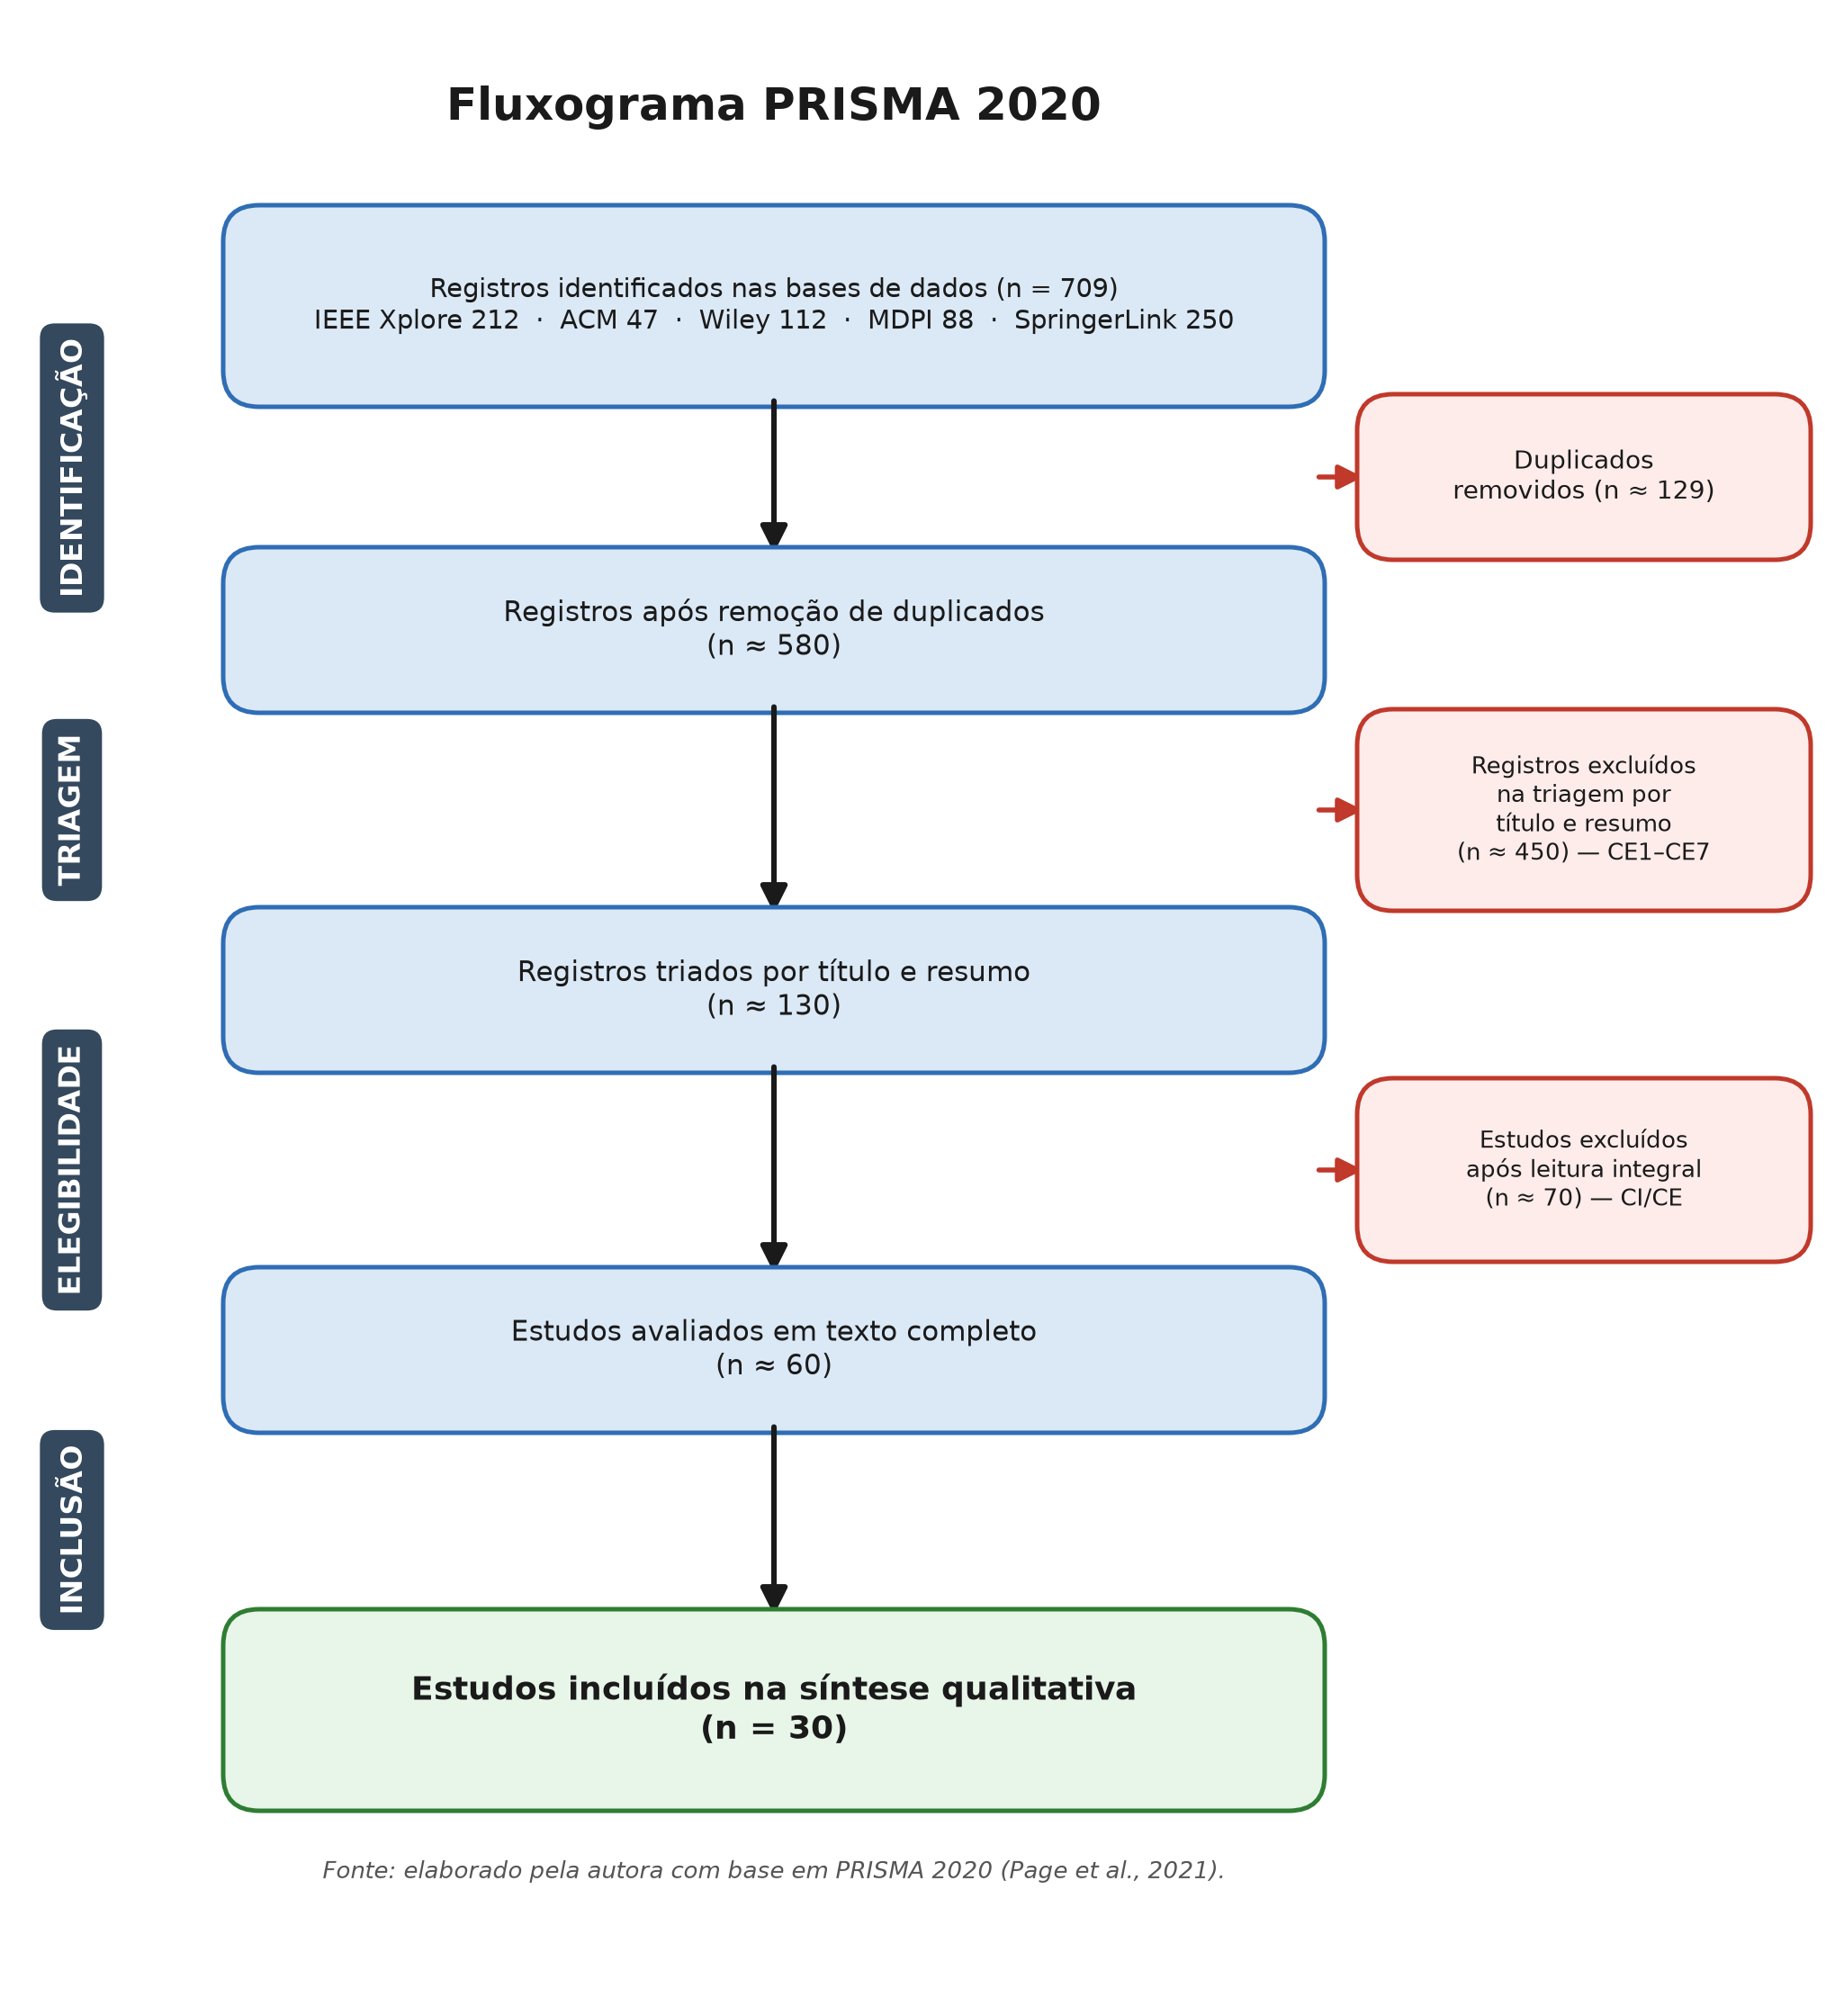
\includegraphics[width=0.7\linewidth]{Figura-PRISMA.png}
    \caption{Fluxo de identificação, triagem e seleção dos estudos conforme as diretrizes PRISMA. Fonte: elaborado pela autora com base em \cite{page2021prisma}.}
    \label{fig:prisma}
\end{figure}

Após a recuperação dos registros, os resultados provenientes das diferentes bases foram consolidados e submetidos à identificação de registros duplicados. Em seguida, foi realizada a triagem por título, resumo e palavras-chave, seguida da avaliação de elegibilidade em texto completo, até a obtenção do conjunto final de estudos incluídos na síntese qualitativa.

\subsubsection{\textit{Pipeline} reprodutível do processo de seleção}

A Tabela~\ref{tab:selecao_pipeline} sumariza quantitativamente o processo reprodutível que
permitiu reduzir o conjunto inicial de 709 estudos até a seleção final de 30 artigos.

\begin{table}[H]
\centering
\caption{\textit{Pipeline} reprodutível do processo de seleção dos estudos.}
\label{tab:selecao_pipeline}
\begin{tabular}{p{5cm} p{4cm} p{5cm}}
\hline
\textbf{Etapa} & \textbf{Quantidade} & \textbf{Descrição} \\
\hline
Resultados brutos iniciais & 709 &
Estudos recuperados após aplicação das queries Q1, Q2 e Q3 nas cinco bases. \\
\hline
Remoção de duplicados & $\sim$580 &
Duplicados eliminados via comparação de DOI, título, autores e ano de publicação. \\
\hline
Triagem por título e resumo & $\sim$130 &
Exclusão de estudos fora do escopo por meio dos critérios CE1, CE2, CE6 e CE7. \\
\hline
Avaliação em texto completo & $\sim$60 &
Leitura integral dos artigos restantes para aplicação rigorosa dos critérios CI/CE. \\
\hline
Estudos incluídos na revisão final & 30 &
Trabalhos selecionados como base definitiva de estudos correlatos desta dissertação. \\
\hline
\end{tabular}
\end{table}

\subsubsection{Processo de curadoria e justificativa da seleção final}

A redução de 709 estudos brutos para os 30 trabalhos finais seguiu um processo de curadoria estruturado em quatro fases, cada uma com critérios e justificativas específicas.

Na primeira fase, a remoção de duplicados identificou artigos indexados em mais de uma base (por exemplo, trabalhos presentes simultaneamente na IEEE Xplore e na SpringerLink). A comparação por DOI eliminou as ocorrências idênticas, enquanto a verificação manual por título e autores detectou versões preliminares (artigos de conferência expandidos em periódicos), retendo apenas a versão mais completa.

Na segunda fase, a triagem por título e resumo aplicou os critérios de exclusão de forma preliminar. Nessa etapa, foram descartados estudos que, embora retornados pelas \textit{queries}, tratavam de temas tangenciais: aplicações de \textit{Federated Learning} em saúde ou agricultura sem contribuição para detecção de intrusões (CE7), trabalhos focados em ataques adversariais sem conexão com inferência de pertencimento (CE2), publicações em idiomas distintos de inglês e português (CE6) e artigos de FL genérico sem relação com segurança (CE1). Essa filtragem reduziu o conjunto de aproximadamente 580 para cerca de 130 estudos.

Na terceira fase, a leitura integral dos textos completos permitiu uma avaliação rigorosa da aderência aos critérios de inclusão. Os estudos retidos nessa etapa foram aqueles que contribuíam diretamente para ao menos um dos eixos da dissertação: (i) arquiteturas de Fed-IDS e algoritmos de agregação federada (CI3), cobrindo desde o trabalho fundacional de McMahan et al. até propostas recentes como F-BIDS e arquiteturas \textit{zero-trust}; (ii) formalização, evolução e avaliação de MIA (CI4), incluindo os marcos de Shokri et al., Nasr et al. e Carlini et al.; e (iii) mecanismos de defesa e mitigação de privacidade (CI5), abrangendo DP-SGD, compressão de gradientes e defesas híbridas.

Na quarta fase, os aproximadamente 60 estudos remanescentes foram avaliados quanto à relevância, impacto e complementaridade. Priorizaram-se trabalhos seminais que introduziram conceitos fundamentais (FedAvg, MIA, DP-SGD, LiRA), revisões sistemáticas que consolidam o estado da arte (Hernandez-Ramos et al., Belenguer et al., Bai et al.) e propostas recentes que avançam a fronteira do conhecimento em defesas híbridas, cenários \textit{non-IID} e auditoria de privacidade em modelos de linguagem. Trabalhos redundantes, com contribuições incrementais ou restritos a cenários sem generalização, foram excluídos nessa etapa final, resultando nos 30 estudos que fundamentam esta dissertação.

Os resultados do processo de seleção são resumidos a seguir:

\begin{itemize}
    \item Registros identificados nas bases de dados: 709;
    \item Registros após remoção de duplicados: $\sim$580;
    \item Registros após triagem por título e resumo: $\sim$130;
    \item Estudos avaliados em texto completo: $\sim$60;
    \item Estudos finais incluídos na revisão: 30.
\end{itemize}

\subsubsection{Estudos selecionados}

A Tabela~\ref{tab:estudos_selecionados} apresenta os 30 estudos que compõem a base final da revisão, organizados cronologicamente. Cada entrada indica os autores, o ano de publicação, o título do trabalho e a \textit{query} responsável por sua recuperação.

\begin{table}[H]
\centering
\scriptsize
\caption{Estudos selecionados na Revisão Sistemática da Literatura.}
\label{tab:estudos_selecionados}
\renewcommand{\arraystretch}{1.2}
\begin{tabular}{p{0.4cm}p{3.0cm}p{0.6cm}p{7.5cm}p{1.2cm}}
\toprule
\textbf{ID} & \textbf{Autor(es)} & \textbf{Ano} & \textbf{Título} & \textbf{Query} \\
\midrule
E1 & Abadi et al. & 2016 & \textit{Deep Learning with Differential Privacy} & Q2 \\
E2 & McMahan et al. & 2017 & \textit{Communication-Efficient Learning of Deep Networks from Decentralized Data} & Q1/Q2 \\
E3 & Shokri et al. & 2017 & \textit{Membership Inference Attacks against Machine Learning Models} & Q2 \\
E4 & Yeom et al. & 2018 & \textit{Privacy Risk in Machine Learning: Analyzing the Connection to Overfitting} & Q2 \\
E5 & Bagdasaryan e Shmatikov & 2019 & \textit{Differential Privacy Has Disparate Impact on Model Accuracy} & Q2 \\
E6 & Nasr et al. & 2019 & \textit{Comprehensive Privacy Analysis of Deep Learning} & Q2 \\
E7 & Li et al. & 2020 & \textit{Federated Optimization in Heterogeneous Networks (FedProx)} & Q1 \\
E8 & Karimireddy et al. & 2020 & \textit{SCAFFOLD: Stochastic Controlled Averaging for Federated Learning} & Q1 \\
E9 & Reddi et al. & 2020 & \textit{Adaptive Federated Optimization} & Q1 \\
E10 & Carlini et al. & 2022 & \textit{Membership Inference Attacks From First Principles} & Q2 \\
E11 & Carlini et al. & 2022 & \textit{Membership Inference Attacks from Likelihood Ratios (LiRA)} & Q2 \\
E12 & Liu et al. & 2022 & \textit{Membership Inference Attacks by Exploiting Loss Trajectory} & Q2 \\
E13 & Mazzone et al. & 2022 & \textit{Repeated Knowledge Distillation with Confidence Masking to Defend against MIAs} & Q2 \\
E14 & Tang et al. & 2022 & \textit{A Federated Learning Method for Network Intrusion Detection} & Q1 \\
E15 & Hernandez-Ramos et al. & 2023 & \textit{Intrusion Detection Based on Federated Learning: A Systematic Review} & Q1 \\
E16 & Aouedi et al. & 2023 & \textit{F-BIDS: Blockchain-Enabled Federated Learning for Intrusion Detection Systems} & Q1 \\
E17 & Lucas et al. & 2023 & \textit{A Comprehensive Survey on Ensemble Learning-Based Intrusion Detection} & Q1 \\
E18 & Li et al. & 2023 & \textit{Communication-Efficient and Privacy-Preserving FL via Gradient Pruning and Differentiated DP} & Q2 \\
E19 & Wu et al. & 2023 & \textit{Efficient Federated Learning on Edge Devices via Model Pruning} & Q2 \\
E20 & Feng et al. & 2023 & \textit{FedPHP: Privacy-Preserving Federated Learning for Network Intrusion Detection} & Q1 \\
E21 & Bai et al. & 2024 & \textit{Membership Inference Attacks and Defenses in Federated Learning: A Survey} & Q2 \\
E22 & Javeed et al. & 2024 & \textit{Zero-Trust Federated Learning-Based Intrusion Detection System} & Q1 \\
E23 & Wei et al. & 2024 & \textit{Gradient Sparsification for Efficient Wireless FL with Differential Privacy} & Q2 \\
E24 & Belenguer et al. & 2025 & \textit{A Survey on the Use of Federated Learning for Intrusion Detection Systems} & Q1 \\
E25 & Niu et al. & 2025 & \textit{Dual Defense: Combining Preemptive Exclusion and Knowledge Distillation to Mitigate MIA} & Q2 \\
E26 & Carlini et al. & 2019 & \textit{The Secret Sharer: Evaluating and Testing Unintended Memorization in Neural Networks} & Q3 \\
E27 & Song et al. & 2019 & \textit{Membership Inference Attacks against Sequence Generation Models} & Q3 \\
E28 & Mattern et al. & 2023 & \textit{Membership Inference Attacks against Language Models via Neighbourhood Comparison} & Q3 \\
E29 & Xie et al. & 2024 & \textit{ReCaLL: Membership Inference via Relative Conditional Log-Likelihoods} & Q3 \\
E30 & Zhang et al. & 2025 & \textit{Min-K\%++: Improved Baseline for Detecting Pre-Training Data from Large Language Models} & Q3 \\
\bottomrule
\end{tabular}
\end{table}

\subsection{Síntese e Contribuição dos Trabalhos Correlatos}

Os resultados da revisão evidenciam que, embora \textit{Federated Learning} seja amplamente
adotado para \textit{Intrusion Detection Systems} distribuídos, ainda existem desafios abertos
associados à privacidade e à exposição de informações sensíveis por meio de ataques de
inferência, como \textit{Membership Inference Attacks}.

Dessa forma, esta dissertação se posiciona na interseção entre Fed-IDS e ataques de
privacidade, contribuindo para a análise e mitigação de \textit{Membership Inference Attacks} em
ambientes federados de detecção de intrusão.

\section{Taxonomia dos Trabalhos Correlatos}
\label{sec:taxonomia}

A literatura relacionada a \textit{Federated Learning} aplicado à detecção de intrusões e aos
desafios de privacidade pode ser organizada em diferentes vertentes de pesquisa.
De modo a estruturar a análise dos trabalhos correlatos e evidenciar lacunas existentes,
esta revisão propõe uma taxonomia composta por quatro eixos principais:

\begin{enumerate}
    \item A transição paradigmática para sistemas de detecção de intrusão federados (Fed-IDS);
    \item A superfície de ataque informativa: ameaças de inferência e vazamento de privacidade;
    \item O dilema da mitigação: o custo da privacidade em ambientes federados;
    \item Síntese crítica e fronteira de pesquisa.
\end{enumerate}

Essa organização permite compreender como os avanços em aprendizado federado para IDS
introduzem simultaneamente benefícios de colaboração distribuída e novos vetores de ataque
relacionados à privacidade.

\subsection{A Transição Paradigmática para a Detecção de Intrusão Federada}

A migração de arquiteturas de IDS centralizadas para federadas é um movimento impulsionado por necessidades técnicas como escalabilidade e latência  e, sobretudo, por imperativos de privacidade. Esta transição é amplamente documentada em revisões sistemáticas, como as de Hernandez-Ramos et al.~\cite{hernandez2023surveyfedids} e Belenguer et al.~\cite{belenguer2025surveyfedids}, que atestam o consenso da comunidade científica sobre os benefícios do FL. Tais estudos, entretanto, também alertam para desafios em aberto, como a robustez em cenários com dados estatisticamente heterogêneos (\textit{non-IID}) e a carência de protocolos de avaliação de segurança padronizados.

A maturidade do campo é evidenciada por um crescente corpo de trabalhos que demonstram a aplicação prática de Fed-IDS. Tang et al.~\cite{tang2022fedids}, por exemplo, validaram a eficácia de um sistema baseado em aprendizado profundo, estabelecendo um \textit{baseline} de desempenho em datasets de referência. Ciente de que ambientes distribuídos introduzem novos vetores de ameaça, a pesquisa tem se voltado para o fortalecimento da confiança no ecossistema federado. Nessa direção, Aouedi et al.~\cite{aouedi2023blockchainids} propuseram o F-BIDS, uma arquitetura que integra FL e \textit{blockchain} para garantir a imutabilidade e a auditabilidade das atualizações de modelo. De forma análoga, Javeed et al.~\cite{javeed2024zerotrust} investigaram a sinergia entre Fed-IDS e o paradigma de segurança \textit{zero-trust}, robustecendo a autenticação dos participantes.

Coletivamente, estes trabalhos estabelecem o Fed-IDS como uma arquitetura funcional e promissora. Contudo, ao endereçar a segurança do repositório de dados, eles implicitamente deslocam o risco para a informação contida nos próprios artefatos de aprendizado que transitam pela rede, uma superfície de ataque mais sutil e complexa.

\subsection{A Superfície de Ataque Informativa: Ameaças de Inferência}

A concepção de que a não-exposição dos dados brutos seria suficiente para garantir a privacidade foi desafiada pelo trabalho seminal de Shokri et al.~\cite{shokri2017mia}, que introduziu e demonstrou a viabilidade dos MIA. A vulnerabilidade reside no fato de que os modelos de ML, ao serem otimizados, internalizam padrões dos dados de treinamento, resultando em um comportamento diferencial  seja no vetor de confiança, na entropia da predição ou na magnitude da perda  quando expostos a amostras que participaram do seu treinamento. Este comportamento, frequentemente acentuado pelo sobreajuste (\textit{overfitting})~\cite{yeom2018privacyrisk}, cria um canal lateral de informação.

No contexto de FL, esta ameaça é exacerbada. A análise pioneira de Nasr et al.~\cite{nasr2019comprehensive} sobre ataques \textit{white-box} foi um marco, ao elucidar como um servidor central pode explorar os gradientes compartilhados para executar MIA com alta precisão, convertendo o processo de agregação em um ponto de vigilância. A sofisticação destes ataques tem crescido exponencialmente, evoluindo de métodos iniciais para técnicas estatisticamente rigorosas, baseadas em princípios primários~\cite{carlini2022firstprinciples}, na razão de verossimilhança (\textit{likelihood ratios})~\cite{carlini2022lira}, e na análise da trajetória da função de perda ao longo do treinamento~\cite{liu2022trajectory}.

Como sistematizado na abrangente revisão de Bai et al.~\cite{bai2024survey}, os MIA deixaram de ser uma curiosidade teórica para se tornarem um desafio fundamental à promessa de privacidade do aprendizado de máquina, exigindo o desenvolvimento de contramedidas robustas.

\subsection{O Dilema da Mitigação: O Custo da Privacidade}

A resposta da comunidade científica à ameaça dos MIA resultou em um espectro de estratégias de defesa, cada uma operando sob um \textit{trade-off} distinto entre privacidade, utilidade e custo computacional.

A abordagem mais formalmente robusta é a \textit{Privacidade Diferencial}, cuja aplicação ao aprendizado profundo foi consolidada por Abadi et al.~\cite{abadi2016dpsgd}. Ao injetar ruído estatístico nos gradientes, a DP oferece garantias matemáticas de privacidade. Contudo, essa formalidade tem um custo: a degradação da acurácia do modelo. Bagdasaryan e Shmatikov~\cite{bagdasaryan2019dpimpact} demonstraram que este impacto é desigual, penalizando desproporcionalmente participantes com dados minoritários, uma questão crítica em cenários \textit{non-IID} típicos de Fed-IDS.

Uma segunda categoria de defesas opera por meio de \textit{regularização e ofuscação}, visando produzir modelos que, por construção, sejam menos suscetíveis à memorização. Técnicas como a destilação de conhecimento (\textit{knowledge distillation})~\cite{mazzone2022kdmask} buscam amenizar a superfície de decisão do modelo, reduzindo o sinal explorável pelos ataques.

Por fim, uma terceira linha de defesa atua na \textit{redução da informação} contida nas atualizações do modelo. Métodos de poda (\textit{pruning})~\cite{wu2023pruningfl} e esparsificação de gradientes~\cite{wei2024gradientsparsification} oferecem um duplo benefício: otimizam a comunicação e limitam a superfície de ataque. A tendência recente, como apontado por Niu et al.~\cite{niu2025dualdefense}, caminha para defesas híbridas, reconhecendo que nenhuma técnica isolada constitui uma panaceia.

\subsection{Síntese Crítica e a Fronteira da Pesquisa}

A análise da literatura revela uma narrativa dialética: o paradigma FL surgiu para resolver a questão da privacidade na centralização de dados, mas, ao fazê-lo, expôs uma nova classe de vulnerabilidades de inferência. Em resposta, um diversificado ferramental de defesas foi desenvolvido, cada qual impondo seus próprios custos e limitações. O estado da arte, portanto, é caracterizado por uma notável fragmentação: as arquiteturas de Fed-IDS são avaliadas por sua utilidade; os ataques de MIA são testados em cenários genéricos; e as defesas são, em sua maioria, analisadas de forma isolada.

Esta dissociação metodológica obscurece as dinâmicas cruciais que governam a aplicação segura de Fed-IDS no mundo real. A lacuna de pesquisa mais significativa reside na ausência de uma \textit{metodologia de auditoria empírica e integrada}, capaz de avaliar de forma rigorosa a interação entre ataque e defesa no domínio específico de detecção de intrusão. Questões fundamentais, portanto, permanecem em aberto:
\begin{enumerate}
    \item Qual a vulnerabilidade quantitativa de sistemas Fed-IDS contemporâneos quando submetidos a ataques de inferência de última geração
    \item Como a eficácia de defesas híbridas  por exemplo, a sinergia entre Privacidade Diferencial e compressão de gradientes  se comporta sob diferentes graus de heterogeneidade de dados (\textit{non-IID})
    \item Qual é a fronteira de Pareto que define o \textit{trade-off} entre a degradação na performance da detecção de intrusões e o ganho em resiliência a ataques de inferência, permitindo uma calibração informada do balanço risco-benefício
\end{enumerate}

\section{Federated Learning}

O \textit{Federated Learning} consolidou-se como um dos paradigmas mais relevantes do aprendizado de máquina contemporâneo ao propor um modelo de treinamento colaborativo no qual os dados permanecem distribuídos entre diferentes clientes. Essa abordagem surgiu em um contexto de crescente preocupação com a privacidade e foi formalizada por McMahan et al., na conferência \textit{Artificial Intelligence and Statistics (AISTATS 2017)}, por meio do algoritmo \textit{Federated Averaging (FedAvg)} \cite{mcmahan2017fedavg}. O princípio fundamental consiste em permitir que múltiplas entidades treinem modelos localmente e enviem apenas parâmetros ou gradientes a um servidor agregador, responsável por consolidar as contribuições em um modelo global. Dessa forma, reduz-se a necessidade de centralização de informações sensíveis, ao mesmo tempo em que se preserva a capacidade de aprendizado em larga escala.

A Figura~\ref{fig:fl_architecture} apresenta a arquitetura geral do \textit{Federated Learning}. Cada organização mantém seus dados locais ($D_{1}$, $D_{2}$, $D_{k}$), que não são compartilhados diretamente. O treinamento ocorre em cada cliente, e os parâmetros resultantes ($m_{1}$, $m_{2}$, $m_{k}$) são transmitidos ao servidor central. Esse servidor realiza a agregação, gerando o modelo global atualizado, que é redistribuído para os clientes em ciclos sucessivos de treinamento.

\begin{figure}[!htbp]
    \centering
    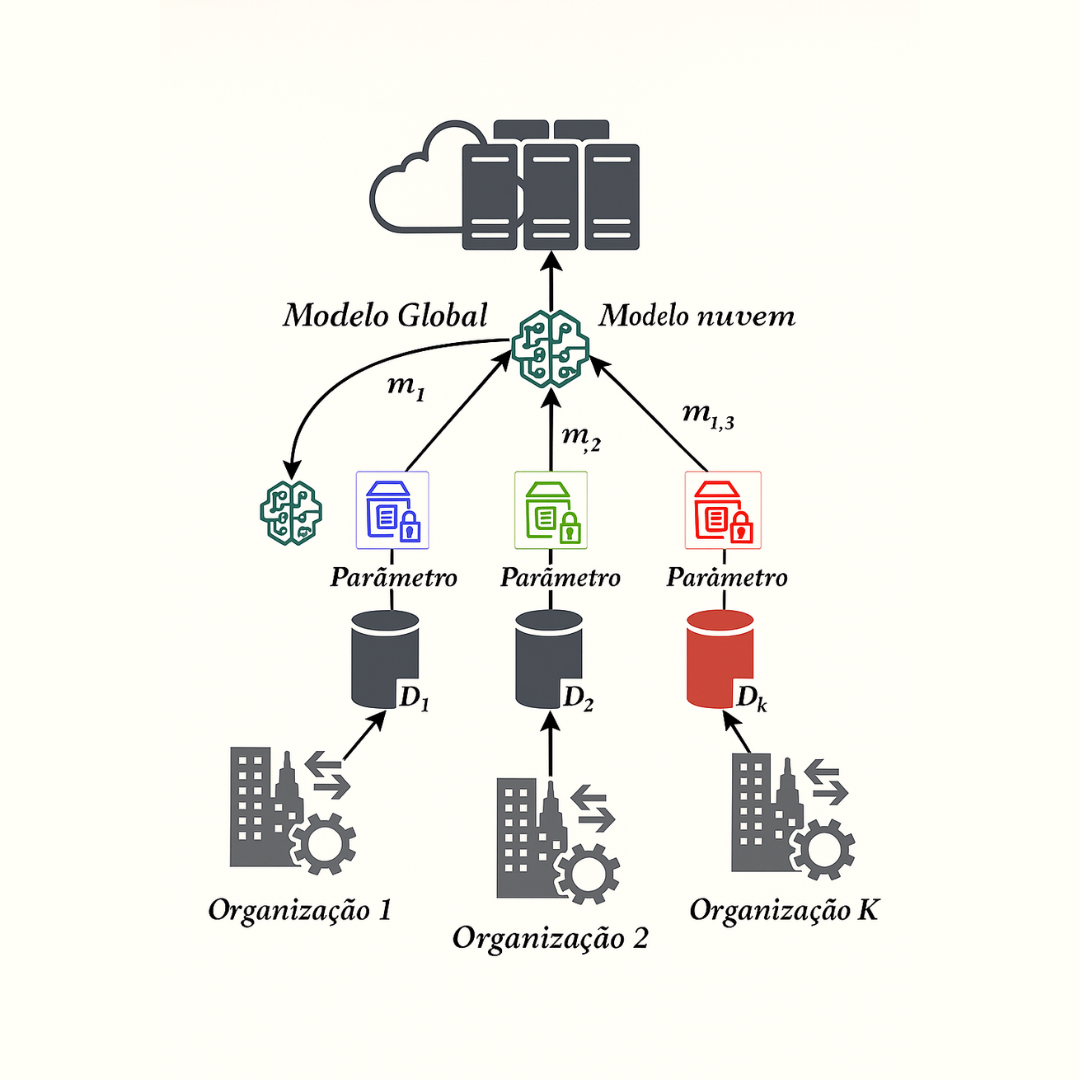
\includegraphics[width=0.6\linewidth]{Figura-1.png}
    \caption{Arquitetura geral do \textit{Federated Learning}. Fonte: elaborado pela autora com base em \cite{mcmahan2017fedavg}.}
    \label{fig:fl_architecture}
\end{figure}


\subsection{Federated Averaging}

O algoritmo \textit{Federated Averaging (FedAvg)} é considerado o marco inicial do \textit{Federated Learning}. Ele foi proposto por McMahan et al. na \textit{AISTATS 2017} \cite{mcmahan2017fedavg} e demonstrou pela primeira vez a viabilidade de treinar redes neurais profundas em ambientes descentralizados. 

O FedAvg baseia-se em um processo iterativo composto por cinco etapas:

\begin{enumerate}[label=(\roman*)]
    \item Inicialização do modelo global no servidor.
    \item Seleção de clientes participantes em cada rodada.
    \item Treinamento local em cada cliente com dados privados.
    \item Envio das atualizações de parâmetros ao servidor.
    \item Agregação das contribuições por meio de uma média ponderada proporcional ao tamanho dos conjuntos de dados locais.
\end{enumerate}

    
Os clientes utilizam o modelo inicial disponibilizado pelo servidor para realizar o treinamento local em seus próprios conjuntos de dados. Ao final de cada rodada, em vez de compartilhar os dados brutos, cada cliente envia apenas os parâmetros atualizados ao servidor agregador. O servidor, por sua vez, aplica uma média ponderada das contribuições recebidas, de acordo com o tamanho dos conjuntos de dados de cada cliente, e gera o modelo global atualizado, que é então redistribuído para todos os participantes.

A atualização do modelo global é definida pela Equação~\ref{eq:fedavg}:

\begin{equation}
w^{t+1} = \sum_{i=1}^{K} \frac{|D_i|}{\sum_{j=1}^{K} |D_j|} \cdot w_i
\label{eq:fedavg}
\end{equation}

\noindent em que:
\begin{itemize}
    \item $w^{t+1}$ representa os parâmetros do modelo global após a rodada $t$;
    \item $K$ é o número total de clientes selecionados para a rodada;
    \item $D_i$ denota o conjunto de dados local do cliente $i$;
    \item $|D_i|$ é a cardinalidade (número de amostras) do conjunto $D_i$;
    \item $w_i$ são os parâmetros do modelo local do cliente $i$ após o treinamento.
\end{itemize}

A expressão realiza uma média ponderada dos modelos locais, em que o peso de cada cliente é proporcional ao tamanho de seu conjunto de dados. A Figura~\ref{fig:fedavg} ilustra, de forma esquemática, esse processo.

\begin{figure}[!htbp]
    \centering
    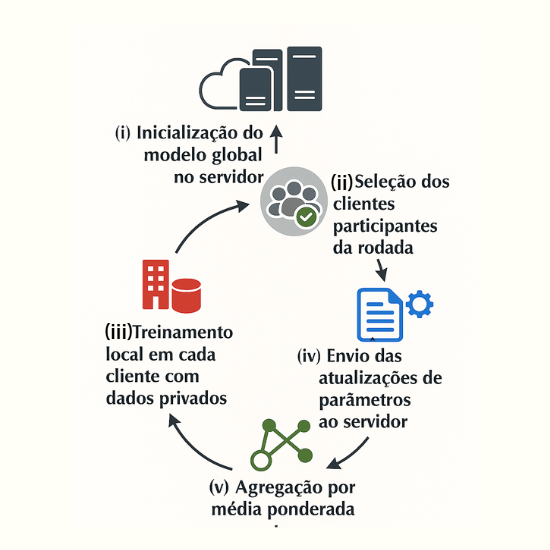
\includegraphics[width=0.5\linewidth]{Figura-2.png}
    \caption{Funcionamento do algoritmo \textit{Federated Averaging}. Fonte: elaborado pela autora com base em \cite{mcmahan2017fedavg}.}
    \label{fig:fedavg}
\end{figure}


\subsection{Federated Proximal}

Para enfrentar as limitações do algoritmo \textit{Federated Averaging} em cenários marcados pela heterogeneidade dos dados, Li et al. apresentaram o \textit{Federated Proximal}, publicado em Proceedings of Machine Learning and Systems (2020) \cite{li2020fedprox}. O FedProx constitui uma extensão natural do FedAvg ao incorporar um termo de regularização proximal no processo de otimização local. Esse termo funciona como uma penalização que restringe a distância entre os parâmetros do modelo local e o modelo global, reduzindo discrepâncias excessivas nas atualizações enviadas ao servidor.

Essa modificação foi concebida para lidar com um dos maiores desafios do Aprendizado Federado: a distribuição não independente e não idêntica dos dados entre os clientes. Em tais cenários, a diversidade estatística das bases locais provoca gradientes altamente divergentes, o que compromete a convergência do modelo e reduz sua acurácia. O FedProx busca mitigar esse efeito ao suavizar as atualizações locais, proporcionando maior estabilidade no processo de agregação.

Além disso, o FedProx preserva a simplicidade estrutural do FedAvg, mantendo o ciclo de treinamento federado tradicional, que compreende inicialização do modelo global, seleção de clientes, treinamento local, envio das atualizações e agregação no servidor. A principal diferença está na inclusão do termo proximal no cálculo da função de perda local, o que amplia a robustez do processo sem demandar alterações significativas na infraestrutura. Embora não elimine totalmente os impactos da heterogeneidade, o FedProx representa um avanço relevante na evolução do Aprendizado Federado, servindo como referência para propostas posteriores voltadas à otimização do desempenho em ambientes complexos e heterogêneos.

\begin{figure}[!htbp]
    \centering
    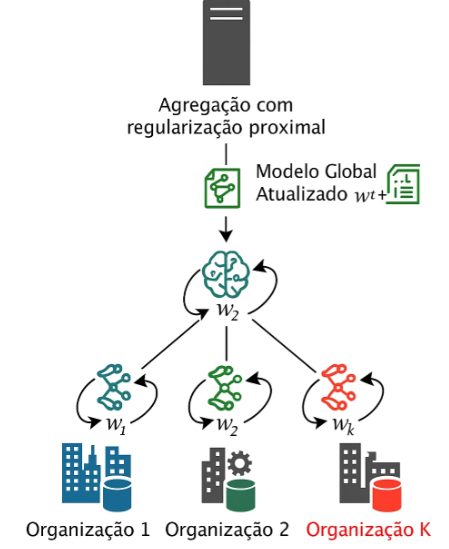
\includegraphics[width=0.4\linewidth]{Figura-3.png}
    \caption{Mecanismo de regularização no \textit{Federated Proximal}. Fonte: elaborado pela autora com base em \cite{li2020fedprox}.}
    \label{fig:fedprox}
\end{figure}

A Figura~\ref{fig:fedprox} ilustra o mecanismo de regularização introduzido pelo FedProx. No FedProx, a função de perda local em cada cliente $i$ passa a ser definida pela Equação~\ref{eq:fedprox}:

\begin{equation}
\mathcal{L}_{i}(w) = f_{i}(w) + \frac{\mu}{2} \| w - w^{t} \|^{2}
\label{eq:fedprox}
\end{equation}

\noindent em que:
\begin{itemize}
    \item $\mathcal{L}_{i}(w)$ é a função de perda local do cliente $i$;
    \item $f_{i}(w)$ representa a função de perda original do cliente $i$;
    \item $\mu$ é o coeficiente de regularização proximal, que controla a intensidade da penalização;
    \item $w$ são os parâmetros do modelo local;
    \item $w^{t}$ são os parâmetros do modelo global na rodada $t$;
    \item $\| w - w^{t} \|^{2}$ é a norma euclidiana ao quadrado entre os parâmetros local e global, que penaliza desvios excessivos.
\end{itemize}

Embora tenha ampliado a robustez do FedAvg, o FedProx não elimina totalmente os impactos da heterogeneidade, mas representa um avanço prático em cenários \textit{non-IID}.

\subsection{Stochastic Controlled Averaging}

O algoritmo \textit{Stochastic Controlled Averaging for Federated Learning (SCAFFOLD)} foi proposto por Karimireddy et al., na \textit{International Conference on Machine Learning (ICML 2020)} \cite{karimireddy2020scaffold}, como uma resposta ao problema do chamado \textit{client drift}. Esse fenômeno ocorre quando os clientes, ao possuírem distribuições de dados heterogêneas, produzem gradientes significativamente distintos entre si, dificultando a convergência do modelo global e reduzindo a acurácia em ambientes descentralizados.  

O SCAFFOLD introduz a utilização de \textit{variáveis de controle estocásticas} que ajustam os gradientes locais antes de sua agregação pelo servidor. A ideia central é compensar o desvio introduzido pelas diferenças estatísticas das bases de cada cliente, permitindo que as atualizações sejam mais consistentes e que os modelos locais se mantenham melhor alinhados ao modelo global. Formalmente, a atualização de parâmetros no cliente $i$ pode ser representada da seguinte forma:

\begin{equation}
w_{i}^{t+1} = w^{t} - \eta \left( g_{i}(w^{t}) - c_{i} + c \right)
\label{eq:scaffold}
\end{equation}

\noindent em que:
\begin{itemize}
    \item $w_{i}^{t+1}$ são os parâmetros atualizados do cliente $i$ após a rodada $t$;
    \item $w^{t}$ representa os parâmetros do modelo global na rodada $t$;
    \item $\eta$ é a taxa de aprendizado;
    \item $g_{i}(w^{t})$ é o gradiente local do cliente $i$, calculado sobre seus dados;
    \item $c_{i}$ corresponde à variável de controle local do cliente $i$, que estima a direção média dos gradientes locais;
    \item $c$ é a variável de controle global mantida pelo servidor, que estima a direção média dos gradientes agregados.
\end{itemize}

A Figura~\ref{fig:scaffold} ilustra, de forma esquemática, como o mecanismo de controle atua na prática: enquanto as atualizações locais tendem a seguir direções divergentes em função da heterogeneidade, as variáveis de controle corrigem esses gradientes, promovendo um alinhamento maior com o modelo global.  

\begin{figure}[H]
    \centering
    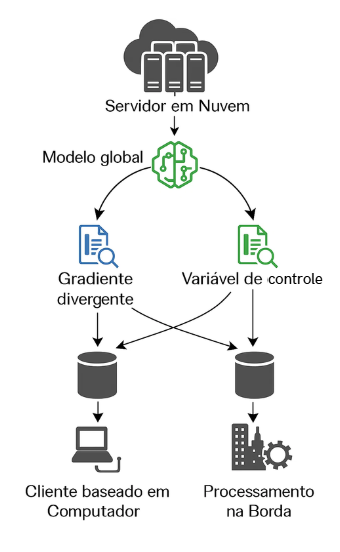
\includegraphics[width=0.4\linewidth]{Figura-4.png}
    \caption{Correção do \textit{client drift} no \textit{SCAFFOLD}. Fonte: elaborado pela autora com base em \cite{karimireddy2020scaffold}.}
    \label{fig:scaffold}
\end{figure}

Embora o SCAFFOLD tenha demonstrado elevada eficácia em cenários com dados não independentes e não idênticos, sua aplicação demanda maior custo de comunicação e armazenamento, devido à necessidade de manutenção das variáveis de controle tanto no servidor quanto em cada cliente. Apesar dessa limitação, representa uma contribuição importante para a evolução do Aprendizado Federado, por reduzir significativamente o impacto da heterogeneidade estatística no processo de treinamento distribuído.  


\subsection{Federated Optimization}

A família de algoritmos denominada \textit{Federated Optimization (FedOpt)} foi apresentada por Reddi et al. nos \textit{Proceedings of the International Conference on Machine Learning (ICML 2020)} \cite{reddi2020fedopt}. Essa proposta buscou superar as limitações do \textit{Federated Averaging (FedAvg)} ao adaptar técnicas consagradas de otimização para o contexto federado, introduzindo variantes que incorporam ajustes dinâmicos na taxa de aprendizado durante a etapa de agregação no servidor.  

Entre as variantes destacam-se o \textit{FedAdam}, o \textit{FedYogi} e o \textit{FedAdagrad}. 
Essas abordagens correspondem à adaptação, para o cenário de aprendizado federado, dos otimizadores 
adaptativos Adam, Yogi e Adagrad. Diferentemente do \textit{FedAvg}, tais métodos permitem que o 
processo de atualização global seja mais estável e robusto em condições adversas, tais como elevado 
número de clientes, heterogeneidade estatística (\textit{non-IID}) e restrições de comunicação. 
Tong et al. \cite{tong2020federated_agm} propuseram os \textit{Federated Adaptive Gradient Methods}, 
com análise teórica sob dados não-IID. Ju et al. \cite{ju2023adafedadam} apresentaram o 
\textit{Adaptive Federated Adam (AdaFedAdam)}, com foco em equidade entre clientes. 
Fekri et al. \cite{fekri2023adaptive_fl} analisaram AdaGrad, Adam e Yogi em cenários federados 
assíncronos, confirmando ganhos estatísticos e computacionais. Esses avanços complementam o marco 
estabelecido por Reddi et al. \cite{reddi2020fedopt}.



De forma geral, o FedOpt segue a atualização global representada pela Equação~\ref{eq:fedopt}:

\begin{equation}
w^{t+1} = w^{t} - \eta \, \hat{m}_{t} \Big/ \left( \sqrt{\hat{v}_{t}} + \epsilon \right)
\label{eq:fedopt}
\end{equation}

\noindent em que:
\begin{itemize}
    \item $w^{t}$ representa os parâmetros do modelo global na rodada $t$;
    \item $\eta$ é a taxa de aprendizado global;
    \item $\hat{m}_{t}$ corresponde ao momento de primeira ordem, que representa a média dos gradientes agregados;
    \item $\hat{v}_{t}$ corresponde ao momento de segunda ordem, que captura a variância acumulada dos gradientes;
    \item $\epsilon$ é um termo de estabilidade numérica que evita divisão por zero.
\end{itemize}

Cada variante do FedOpt se diferencia pela forma como calcula e atualiza esses momentos, adaptando o processo de otimização às características dos dados e às condições de comunicação.

A Figura~\ref{fig:fedopt} ilustra de forma conceitual o funcionamento do FedOpt, mostrando como os parâmetros locais enviados pelos clientes são processados no servidor utilizando diferentes estratégias de otimização adaptativa antes da redistribuição do modelo global atualizado.  

\begin{figure}[H]
    \centering
    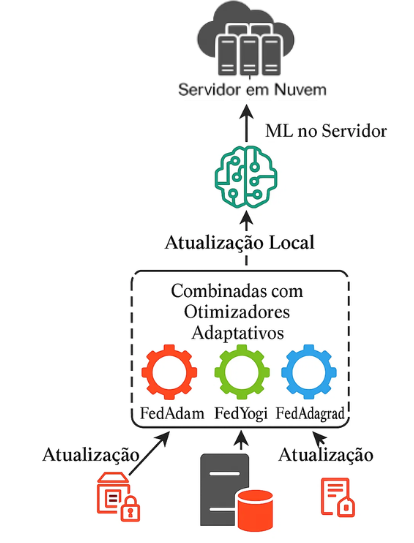
\includegraphics[width=0.4\linewidth]{Figura-5.png}
    \caption{Funcionamento do \textit{Federated Optimization} (FedOpt). Fonte: elaborado pela autora com base em \cite{reddi2020fedopt}.}
    \label{fig:fedopt}
\end{figure}

O FedOpt demonstrou ganhos expressivos em cenários desafiadores, proporcionando convergência mais rápida e modelos mais estáveis em comparação ao FedAvg. No entanto, essas variantes introduzem maior complexidade computacional no servidor, além de dependerem da escolha adequada de hiperparâmetros de otimização. Ainda assim, constituem um marco relevante na literatura do Aprendizado Federado, estabelecendo um ponto de equilíbrio entre robustez, eficiência estatística e custo de comunicação.  

\subsection{Desafios em Ambientes non-IID}

A heterogeneidade estatística dos dados, caracterizada pela condição 
\textit{non-independent and identically distributed (non-IID)}, constitui um dos maiores 
desafios no âmbito do \textit{Federated Learning}. Esse fenômeno ocorre quando os clientes 
participantes possuem distribuições de dados distintas, o que resulta em gradientes locais 
divergentes e, consequentemente, em dificuldades de convergência do modelo global. 
Além de comprometer a estabilidade, tal cenário impacta diretamente a acurácia final, 
limitando a efetividade das aplicações do aprendizado federado em ambientes reais.  

Diversos estudos buscaram mitigar os efeitos dessa heterogeneidade. Entre as propostas 
recentes, destaca-se o \textit{Federated Learning with Non-IID Data via Review Learning (FedRL)}, 
apresentado por Kang e Li em 2022. O FedRL introduz um mecanismo de aprendizado por reforço 
que atua como agente de revisão das atualizações enviadas pelos clientes. Esse agente é capaz 
de reter informações históricas e, com base nelas, ajustar dinamicamente o processo de 
agregação no servidor. Essa estratégia resulta em ganhos significativos de estabilidade e 
aceleração da convergência, demonstrando desempenho superior em cenários com dados altamente 
não homogêneos \cite{kang2022fedrl}.  


À esquerda, observa-se a condição IID, na qual os modelos locais mantêm consistência entre si, 
favorecendo a agregação das atualizações e a rápida convergência global. 
À direita, a condição non-IID provoca divergências significativas entre os modelos locais, 
o que dificulta a estabilização do processo de treinamento e compromete a performance final 
do modelo global.

\begin{figure}[H]
    \centering
    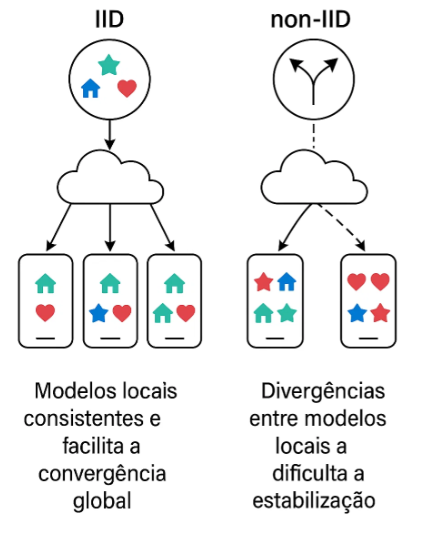
\includegraphics[width=0.4\linewidth]{Figura-6.png}
    \caption{Impacto da heterogeneidade de dados no \textit{Federated Learning}. Fonte: elaborado pela autora.}
    \label{fig:non_iid}
\end{figure}

Embora soluções como FedProx, SCAFFOLD, FedOpt e FedRL avancem na mitigação dos impactos 
dos dados non-IID, ainda não se consolidou uma solução definitiva para o problema. A 
heterogeneidade permanece como uma barreira teórica e prática, exigindo esforços contínuos 
da comunidade científica para desenvolver mecanismos de otimização e agregação capazes de 
garantir robustez, eficiência estatística e estabilidade em cenários distribuídos reais.

\section{Membership Inference Attacks}
Os MIA constituem uma classe de ataques de privacidade cujo objetivo é inferir se uma instância específica de dados integrou o conjunto de treinamento de um modelo. A relevância desse problema decorre do fato de que a mera capacidade de inferir a participação de um dado pode violar a privacidade de indivíduos e organizações, sobretudo em domínios sensíveis, como saúde, finanças e segurança. O trabalho seminal de Shokri et al., apresentado no \textit{IEEE Symposium on Security and Privacy} (2017), demonstrou a viabilidade prática de ataques de inferência de pertencimento em modelos supervisionados, inaugurando uma linha de pesquisa hoje consolidada \cite{shokri2017mia}. Pesquisas subsequentes analisaram a conexão entre \textit{overfitting} e risco de privacidade \cite{yeom2018privacyrisk}, propuseram ataques em cenários \textit{white-box} centralizados e federados \cite{nasr2019comprehensive}, e formalizaram novas estruturas de ataque, como a abordagem \textit{from first principles} \cite{carlini2022firstprinciples} e a exploração da trajetória de perda (\textit{loss trajectory}) ao longo do treinamento \cite{liu2022trajectory}. Estudos de síntese recentes reforçam a importância do tema e sistematizam resultados, ameaças e defesas \cite{bai2024survey}.


A capacidade de inferir a participação de amostras no treinamento expõe sérias implicações de segurança e privacidade, sobretudo em contextos que envolvem dados sensíveis, como registros médicos, informações financeiras ou bases de identificação pessoal. A vulnerabilidade decorre principalmente do fenômeno de \textit{overfitting}, no qual o modelo tende a memorizar exemplos de treinamento em vez de apenas aprender padrões generalizáveis, aumentando o risco de vazamento de informações.

\subsection{Conceito e Funcionamento dos \textit{Membership Inference Attacks}}

Os MIA representam uma das classes mais estudadas de ataques de privacidade em aprendizado de máquina, tendo como objetivo determinar se uma instância específica de dado foi utilizada no processo de treinamento de um modelo. A relevância desse problema está no fato de que, mesmo sem acesso direto aos dados brutos, um adversário capaz de inferir a participação de um exemplo em um conjunto de treinamento já compromete a privacidade dos indivíduos envolvidos, expondo informações potencialmente sensíveis. 

O conceito foi formalizado por Shokri et al., no \textit{IEEE Symposium on Security and Privacy (2017)} \cite{shokri2017mia}, em um trabalho seminal que demonstrou a vulnerabilidade de modelos de classificação supervisionada a esse tipo de ataque. A intuição explorada consiste na diferença de comportamento entre as previsões realizadas sobre exemplos de treino e exemplos não vistos. Modelos com sobreajuste (\textit{overfitting}), em particular, tendem a memorizar instâncias específicas, apresentando maior confiança ou padrões de saída distintos quando confrontados com dados utilizados no treinamento.

Um ataque de inferência de pertencimento pode ser definido como uma função $A(x)$ que, dado um exemplo $x$ e o acesso ao modelo-alvo $M$, busca inferir se $x$ pertence ao conjunto de treinamento $D_{train}$:

\begin{equation}
A(x) = 
\begin{cases}
1, & \text{se } x \in D_{train} \\
0, & \text{se } x \notin D_{train}
\end{cases}
\label{eq:mia}
\end{equation}

Outra forma recorrente de formalização, utilizada em trabalhos posteriores, consiste na definição do \textit{ganho do adversário} (\textit{advantage}), que mede a diferença entre as probabilidades de acerto do atacante quando confrontado com instâncias membros e não membros \cite{yeom2018privacyrisk}:

\begin{equation}
Adv(A) = \left| P[A(x) = 1 \mid x \in D_{train}] - P[A(x) = 1 \mid x \notin D_{train}] \right|
\label{eq:advantage}
\end{equation}

Essa métrica quantifica a eficácia do ataque e estabelece uma base comparativa entre diferentes métodos.

O método clássico proposto por Shokri et al. baseia-se no uso de \textit{shadow models}. Nesse procedimento, o adversário treina múltiplos modelos auxiliares em dados de distribuição semelhante à do modelo-alvo. Como nesses cenários o adversário tem pleno conhecimento de quais exemplos foram incluídos ou não no treinamento, é possível observar o comportamento típico das previsões sobre instâncias membros e não membros. Com base nessas observações, constrói-se um \textit{classificador de ataque}, que aprende a distinguir os dois casos. Esse classificador é então utilizado para consultar o modelo-alvo, inferindo se uma nova instância pertenceu ao conjunto de treinamento.

Esse processo pode ser descrito em três etapas principais, conforme a literatura \cite{shokri2017mia}, \cite{truex2019mia} e \cite{carlini2022firstprinciples}:

\begin{enumerate}
    \item \textbf{Treinamento de modelos sombra:} o adversário utiliza dados auxiliares para treinar modelos semelhantes ao modelo-alvo, controlando a composição dos conjuntos de treino e teste.
    \item \textbf{Construção do classificador de ataque:} as respostas dos modelos sombra são utilizadas para treinar um modelo de ataque, capaz de distinguir instâncias pertencentes ao treinamento daquelas externas.
    \item \textbf{Aplicação ao modelo-alvo:} o classificador de ataque é utilizado para consultar o modelo-alvo e decidir sobre a participação de novas amostras.
\end{enumerate}

A Figura~\ref{fig:mia_conceito} ilustra o funcionamento conceitual desse processo, evidenciando como os modelos sombra e o classificador de ataque se articulam para explorar a superfície de vulnerabilidade do modelo-alvo. O adversário treina modelos sombra em dados auxiliares e, a partir de suas saídas, constrói um classificador de ataque 
    que é posteriormente aplicado ao modelo-alvo para inferir se uma amostra pertenceu ao conjunto de treinamento.

\begin{figure}[H]
    \centering
    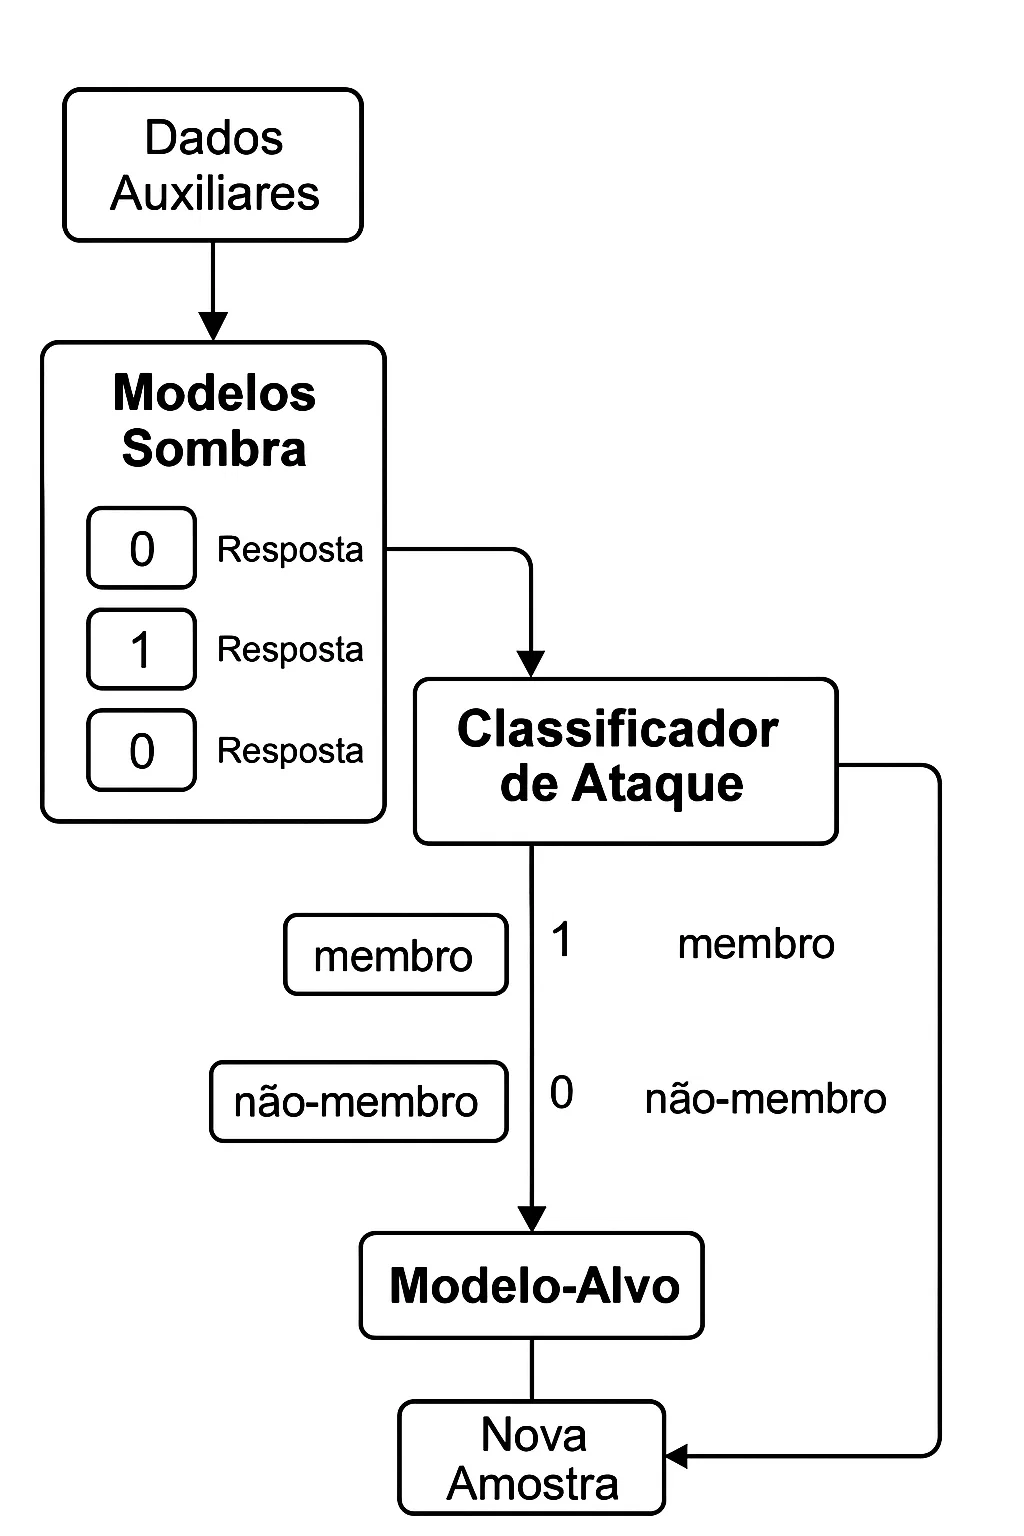
\includegraphics[width=0.4\linewidth]{Figura-7.png}
    \caption{Conceito de um \textit{Membership Inference Attack} (MIA). Fonte: elaborado pela autora com base em \cite{shokri2017mia}.}
    \label{fig:mia_conceito}
\end{figure}

A literatura subsequente demonstrou que a eficácia dos MIA não se restringe ao uso de modelos sombra. Ataques mais recentes exploram métricas simples, como a função de perda (\textit{loss}) ou a entropia das distribuições de saída \cite{yeom2018privacyrisk, song2019mia}. Nesses casos, a hipótese é que exemplos membros tendem a apresentar valores de perda significativamente menores do que exemplos não membros. Essa linha de pesquisa levou ao desenvolvimento de técnicas mais avançadas, como o \textit{Likelihood Ratio Attack (LiRA)}, proposto por Carlini et al. em \textit{USENIX Security 2022} \cite{carlini2022lira}, que se tornou o novo padrão de avaliação da eficácia dos MIA por sua robustez estatística e baixo índice de falsos positivos.

Os impactos práticos desses ataques são vastos. Em cenários de saúde, é possível inferir se registros clínicos de pacientes foram incluídos em bases utilizadas para treinar sistemas de diagnóstico auxiliado por IA, implicando em riscos éticos e legais. Em finanças, ataques desse tipo podem expor a inclusão de dados de clientes em modelos de análise de crédito ou de detecção de fraude. Já em contextos de autenticação biométrica, como reconhecimento facial ou de voz, a inferência bem-sucedida de participação de amostras viola diretamente a privacidade dos indivíduos. Esses exemplos demonstram que os MIA não constituem apenas uma ameaça teórica, mas configuram um risco concreto e de alta relevância prática.


\subsection{Tipologia dos Ataques}
\label{subsec:mia_taxonomia}

Os \textit{Membership Inference Attacks} podem ser classificados segundo diferentes dimensões, relacionadas à capacidade do adversário, ao tipo de acesso ao modelo e à forma de interação com o processo de treinamento.

\subsubsection{\textbf{Acesso ao modelo.}}
No cenário \textit{black-box}, o adversário observa apenas as saídas do modelo, como pontuações de probabilidade ou rótulos finais. Essa é a configuração clássica introduzida por Shokri et al. \cite{shokri2017mia}, que assume que o atacante não dispõe de informações internas do sistema. 
No cenário \textit{white-box}, por outro lado, o adversário tem acesso a parâmetros internos, gradientes ou estados intermediários do treinamento. Nasr et al. \cite{nasr2019comprehensive} demonstraram que ataques dessa natureza podem ser tanto passivos quanto ativos, explorando gradientes locais e mensagens trocadas durante rounds de treinamento centralizados ou federados.

\subsubsection{\textbf{Modalidade de interação.}}
Um ataque é classificado como \textit{passivo} quando o adversário se limita a observar as consultas ao modelo e suas respectivas respostas, sem alterar o processo de treinamento. 
Já ataques \textit{ativos} envolvem manipulação direta, seja pela inserção de consultas adversariais ou pela interferência em rounds de aprendizado federado, ampliando a superfície de ataque e aumentando a probabilidade de sucesso \cite{nasr2019comprehensive}.

\subsubsection{\textbf{Granularidade da inferência.}}
Ataques podem operar sobre \textit{instâncias únicas}, avaliando a participação de um único exemplo $x$ no conjunto de treinamento, ou em \textit{lotes de instâncias} (\textit{batch-wise}). Essa última modalidade utiliza múltiplas amostras correlatas para reforçar o sinal estatístico, aumentando o poder do ataque. Liu et al. \cite{liu2022trajectory} exploram esse princípio ao propor ataques baseados na análise da trajetória de perda (\textit{loss trajectory}) de várias amostras ao longo do processo de treinamento.


A figura ~\ref{fig:mia_taxonomia} é a representação esquemática dos cenários de ataque. 
    A esquerda, configuração \textit{black-box}, em que o adversário acessa apenas as saídas do modelo. 
    À direita, configuração \textit{white-box}, em que há acesso a parâmetros internos, gradientes ou atualizações.
\begin{figure}[H]
    \centering
    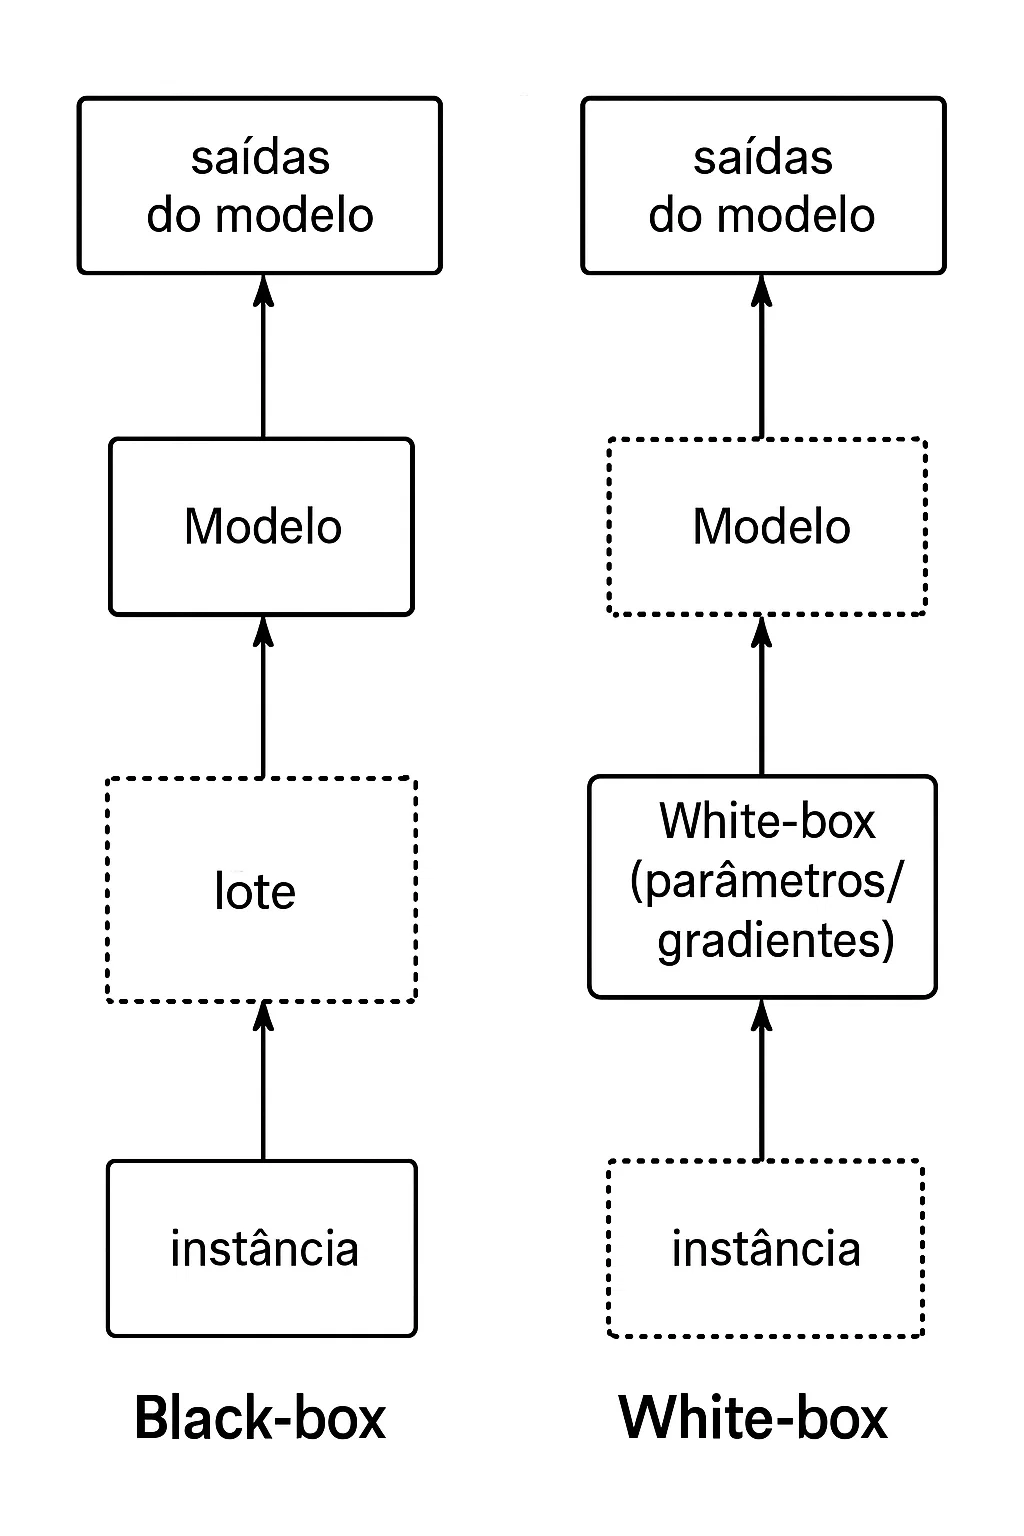
\includegraphics[width=0.4\linewidth]{Figura-8.png}
    \caption{Visão comparativa dos ataques MIA em modo \textit{black-box} e \textit{white-box}. Fonte: elaborado pela autora com base em \cite{nasr2019comprehensive}.}
    \label{fig:mia_taxonomia}
\end{figure}

A literatura recente consolidou formulações mais robustas e com menor taxa de falso positivo. Carlini et al. propuseram uma análise \textit{from first principles} \cite{carlini2022firstprinciples}, reexaminando pressupostos de ataques anteriores e estabelecendo critérios estatísticos mais sólidos para a decisão de pertencimento. Em paralelo, Liu et al. \cite{liu2022trajectory} mostraram que a evolução temporal da função de perda para uma instância específica ao longo do treinamento (\textit{loss trajectory}) constitui um sinal informativo adicional, explorável por adversários para realizar inferência de pertencimento.

No contexto do Aprendizado Federado, ataques \textit{white-box}, sejam passivos ou ativos, exploram gradientes, atualizações locais e dinâmicas de agregação, ampliando o risco de vazamento, sobretudo em cenários com forte heterogeneidade dos dados. Esse problema é ressaltado na análise abrangente de Nasr et al. \cite{nasr2019comprehensive} e nas revisões sistemáticas mais recentes \cite{bai2024survey}, que apontam a maturidade e a diversidade das técnicas de ataque como um dos maiores desafios contemporâneos para a privacidade em sistemas distribuídos.


\subsection{Métricas de avaliação e protocolos}
\label{subsec:mia_metricas}

A avaliação de ataques de inferência de pertencimento demanda métricas que capturem não apenas a capacidade preditiva do ataque, mas também o seu impacto em termos de privacidade. Diferentemente de tarefas tradicionais de classificação, em que o objetivo é maximizar a acurácia sobre classes previamente definidas, em MIA a preocupação central está em quantificar o risco de que a participação de indivíduos em um conjunto de treinamento seja revelada de maneira confiável. Para esse fim, a literatura consolidou um conjunto de métricas específicas.

\subsubsection{\textbf{Taxa de verdadeiros positivos sob baixa taxa de falsos positivos (TPR@FPR)}}
Essa métrica mede a proporção de acertos do ataque em identificar corretamente instâncias que pertenceram ao conjunto de treinamento (verdadeiros positivos), considerando apenas cenários em que a taxa de falsos positivos (casos em que instâncias externas são incorretamente classificadas como membros) permanece controlada. O uso do TPR@FPR é relevante porque, em contextos de privacidade, mesmo baixos índices de falsos positivos podem comprometer a credibilidade do ataque. Trabalhos como o de Nasr et al. \cite{nasr2019comprehensive} exploram extensivamente essa métrica ao avaliar ataques em configurações centralizadas e federadas.

\subsubsection{\textbf{Área sob a curva ROC (AUC-ROC)}}
A AUC-ROC é uma métrica clássica que avalia a capacidade discriminativa do classificador de ataque ao variar o limiar de decisão. Quanto mais próximo de 1 for o valor da área, maior a separabilidade entre exemplos membros e não-membros. No contexto de MIA, valores de AUC acima de 0,5 (que representa o acaso) já indicam que o ataque é capaz de extrair algum sinal de pertencimento. Essa métrica é particularmente utilizada em revisões recentes, como a de Bai et al. \cite{bai2024survey}, para comparar a eficácia de diferentes métodos de ataque em múltiplos cenários.

\subsubsection{\textbf{Acurácia do classificador de ataque}}
Assim como em tarefas convencionais de aprendizado supervisionado, a acurácia mede a proporção de acertos do classificador de ataque sobre o total de exemplos avaliados. Apesar de sua simplicidade, a acurácia isolada pode ser enganosa em bases desbalanceadas, já que não diferencia entre os tipos de erro (falsos positivos e falsos negativos). Por esse motivo, costuma ser utilizada em conjunto com métricas mais robustas, como AUC e TPR@FPR.

\subsubsection{\textbf{Vantagem do atacante (Advantage)}}
Definido formalmente por Yeom et al. \cite{yeom2018privacyrisk}, o \textit{advantage} é uma métrica específica para ataques de privacidade. Trata-se da diferença absoluta entre a probabilidade de o ataque predizer “membro” corretamente para instâncias de treino e a probabilidade de o mesmo ocorrer para instâncias fora do treino, conforme descrito na Equação \ref{eq:advantage}. Valores elevados de \textit{advantage} indicam maior poder do ataque, refletindo a capacidade do adversário em explorar discrepâncias comportamentais do modelo.

\subsubsection{\textbf{Protocolos experimentais}}
Além da escolha das métricas, é prática consolidada adotar protocolos de avaliação que estratifiquem os resultados segundo fatores críticos. Entre os mais recorrentes destacam-se:


\begin{enumerate}[label=(\roman*)]
    \item O nível de \textit{overfitting} do modelo, uma vez que maior sobreajuste tende a aumentar a vulnerabilidade a MIA;
    \item A proporção entre conjuntos de treino e teste, que afeta a disponibilidade de exemplos externos;
    \item O cenário de acesso do adversário, diferenciando ataques em configurações \textit{black-box} e \textit{white-box}.
\end{enumerate}

No contexto do Aprendizado Federado, investigações recentes ressaltam a importância de protocolos adicionais que incluam:

\begin{itemize}
    \item A influência de diferentes algoritmos de agregação (\textit{FedAvg}, \textit{FedProx}, \textit{SCAFFOLD}, \textit{FedOpt});
    \item A frequência e a estratégia de seleção de clientes em cada rodada de treinamento;
    \item O grau de heterogeneidade estatística (\textit{non-IID}) entre as bases locais.
\end{itemize}

Essas variáveis, quando combinadas, alteram significativamente a superfície de ataque e devem ser consideradas para que a avaliação seja representativa \cite{nasr2019comprehensive,bai2024survey}.


\begin{table}[H]
\centering
\caption{Principais métricas para avaliação de ataques de inferência de pertencimento.}
\begin{tabular}{|p{3cm}|p{9cm}|}
\hline
\textbf{Métrica} & \textbf{Descrição} \\ \hline
TPR@FPR & Mede a taxa de verdadeiros positivos do ataque sob restrições de baixa taxa de falsos positivos. Essencial em cenários de privacidade. \\ \hline
AUC-ROC & Avalia a separabilidade entre membros e não-membros ao variar o limiar de decisão. Valores próximos de 1 indicam ataques altamente eficazes. \\ \hline
Acurácia & Percentual total de acertos do classificador de ataque. Métrica simples, mas pode ser enviesada em cenários desbalanceados. \\ \hline
Advantage & Diferença absoluta entre a taxa de sucesso do ataque em membros e não-membros. Métrica formal específica para MIA. \\ \hline
\end{tabular}
\label{tab:mia_metrics}
\end{table}

Em síntese, a avaliação dos ataques de inferência de pertencimento não deve ser feita de maneira unidimensional, mas sim combinando métricas estatísticas clássicas com medidas específicas de privacidade, em protocolos que reflitam a diversidade de cenários práticos. Essa abordagem integrada permite não apenas mensurar a eficácia dos ataques, mas também compreender em que condições os riscos de privacidade se tornam mais críticos.

\subsection{Intrusion Detection Systems (IDS) e Fed-IDS}
\label{subsec:ids_fedids}

Os IDS constituem um dos principais mecanismos de defesa em cibersegurança, sendo responsáveis por monitorar tráfego de rede, identificar comportamentos anômalos e detectar padrões característicos de ataques. Tradicionalmente, os IDS assumem arquiteturas centralizadas, em que dados de diferentes pontos da rede são coletados em um servidor central e processados por algoritmos de detecção baseados em assinaturas ou em modelos de aprendizado de máquina. Apesar da eficácia, esse paradigma centralizado apresenta limitações em termos de escalabilidade, latência e, sobretudo, privacidade, já que a centralização de grandes volumes de tráfego sensível aumenta a superfície de ataque e o risco de exposição de dados confidenciais.

O avanço de tecnologias distribuídas e de ambientes heterogêneos, como redes de \textit{Internet of Things} (IoT) e sistemas industriais inteligentes, trouxe novos desafios para os IDS. Nesses contextos, a coleta de dados ocorre de forma descentralizada, em dispositivos com capacidades computacionais limitadas, e frequentemente sob restrições de comunicação. Essa distribuição de dados, somada à necessidade de preservação de privacidade, inviabiliza a centralização completa das informações e demanda abordagens mais flexíveis e seguras.

Nesse cenário, o FL surge como alternativa promissora, permitindo a construção de modelos colaborativos de detecção de intrusões sem que os dados brutos precisem ser compartilhados. Em um Fed-IDS, cada cliente  por exemplo, um roteador, sensor IoT ou servidor de borda  treina localmente um modelo com seus próprios registros de tráfego e envia apenas parâmetros ou gradientes ao servidor central. Esse servidor, por sua vez, realiza a agregação das atualizações e redistribui o modelo global atualizado a todos os participantes. Dessa forma, preserva-se a privacidade dos dados de rede, ao mesmo tempo em que se mantém a colaboração entre múltiplos domínios administrativos.

Revisões recentes reforçam o potencial dessa abordagem. Hernandez-Ramos et al. \cite{hernandez2023surveyfedids} apresentaram uma análise sistemática do uso de FL em IDS, destacando ganhos de privacidade e limitações de desempenho. Belenguer et al. \cite{belenguer2025surveyfedids} ampliaram a discussão ao sistematizar os trabalhos aplicados em diferentes datasets clássicos, como CIC-IDS2017 e UNSW-NB15. Além disso, Aouedi et al. \cite{aouedi2023blockchainids} exploraram a integração de blockchain com Fed-IDS, propondo maior confiabilidade nas trocas de parâmetros, enquanto Javeed et al. \cite{javeed2024zerotrust} propuseram arquiteturas baseadas em \textit{zero-trust} para aumentar a robustez contra ataques internos. Esses esforços demonstram a relevância e a maturidade do campo, ao mesmo tempo em que evidenciam lacunas relacionadas a ataques de privacidade, como os MIA, ainda pouco explorados em profundidade no domínio de Fed-IDS.

\begin{figure}[H]
    \centering
    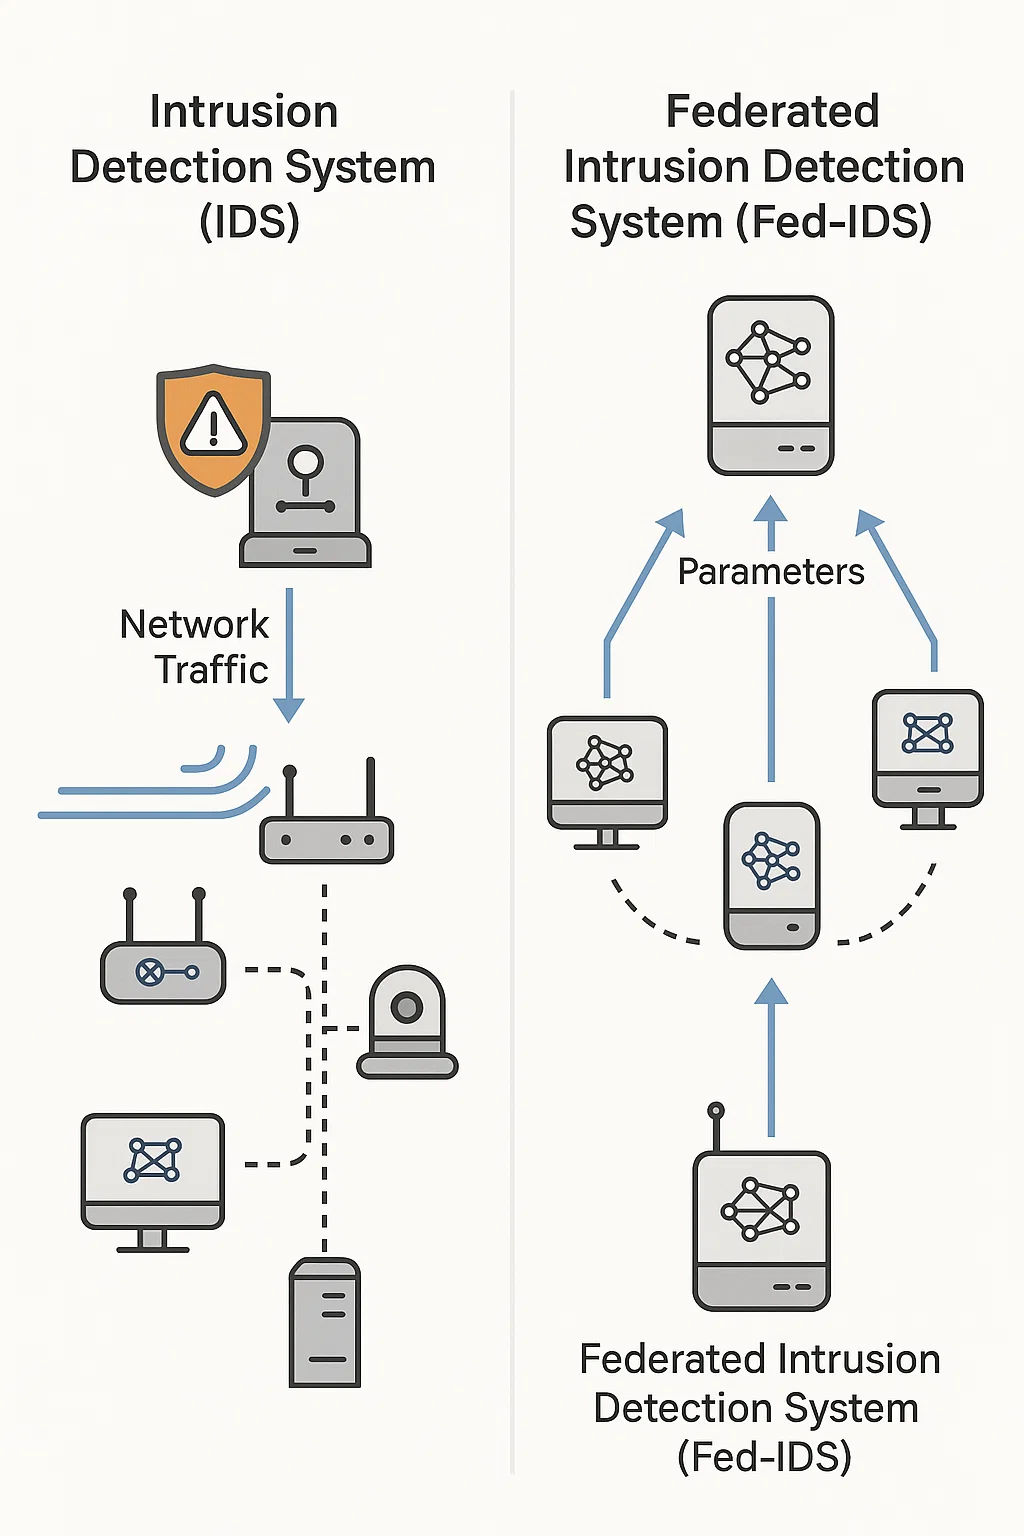
\includegraphics[width=0.5\linewidth]{Figura-9.png}
    \caption{Arquitetura conceitual de um Fed-IDS. Fonte: elaborado pela autora.}
    \label{fig:fedids}
\end{figure}
\subsection{Defesas Híbridas: \textit{Differential Privacy}, \textit{AdaMixup} e Compressão de Gradientes}
\label{subsec:defesas_hibridas}

Os ataques de inferência de pertencimento revelam vulnerabilidades críticas no uso de Aprendizado Federado em sistemas sensíveis como IDS. Nesse contexto, diferentes linhas de defesa têm sido propostas, buscando preservar a utilidade do modelo ao mesmo tempo em que reduzem o risco de vazamento de informações. Entre elas, destacam-se as defesas baseadas em privacidade diferencial, técnicas de regularização por mistura de dados e métodos de compressão e quantização de gradientes.À esquerda, as defesas aplicadas isoladamente (\textit{DP-SGD}, regularização por mistura de dados e compressão/quantização de gradientes) apresentam coberturas parciais da superfície de vazamento e diferentes custos de utilidade. À direita, a defesa híbrida combina mecanismos complementares, alcançando melhor equilíbrio entre utilidade e privacidade no contexto de ataques de inferência de pertencimento.
\begin{figure}[H]
    \centering
    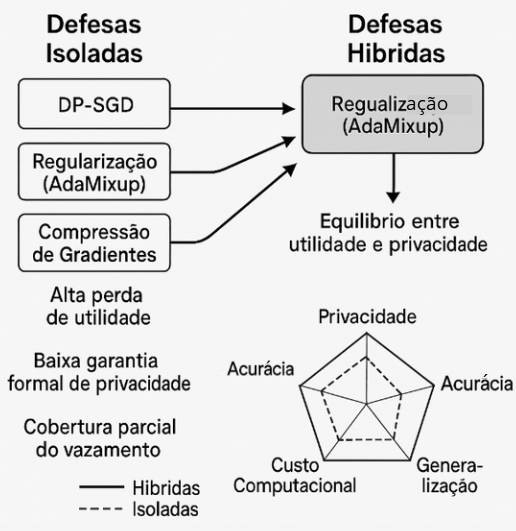
\includegraphics[width=0.5\linewidth]{Figura-11.png}
    \caption{Comparativo conceitual entre defesas isoladas e defesas híbridas em Fed-IDS. Fonte: elaborado pela autora.}
    \label{fig:comparativo_defesas}
\end{figure}
\subsubsection{\textbf{Differential Privacy (DP-SGD)}}
A privacidade diferencial constitui o arcabouço teórico mais difundido para a proteção de dados em aprendizado de máquina. Introduzida no contexto de redes neurais por Abadi et al. \cite{abadi2016dpsgd}, o DP-SGD adiciona ruído calibrado aos gradientes e aplica mecanismos de \textit{clipping} às atualizações, limitando a influência de cada amostra individual sobre o modelo final. Embora eficaz, trabalhos como Bagdasaryan e Shmatikov \cite{bagdasaryan2019dpimpact} mostram que a aplicação de DP pode impactar desproporcionalmente a acurácia em cenários de dados não balanceados, exigindo calibragem cuidadosa do parâmetro $\epsilon$.

\subsubsection{\textbf{AdaMixup e regularização por mistura de dados}}
Outra linha de defesa consiste em utilizar estratégias de regularização que dificultem a memorização de exemplos específicos. O AdaMixup, inspirado em técnicas de \textit{data augmentation}, cria combinações lineares dinâmicas de exemplos durante o treinamento, reduzindo a exposição de instâncias individuais e mitigando a eficácia dos MIA. Trabalhos recentes exploram essa abordagem em contextos federados, apontando ganhos de robustez em cenários \textit{non-IID}. Li et al. \cite{li2023gradientpruning}, por exemplo, exploram estratégias adaptativas de poda de gradientes combinadas com mecanismos de privacidade para reduzir o vazamento de informações sensíveis.

\subsubsection{\textbf{Compressão e quantização de gradientes}}
A compressão e a quantização de gradientes surgem como defesas complementares, com duplo objetivo: reduzir o custo de comunicação em ambientes distribuídos e limitar a quantidade de informação que pode ser explorada por adversários. Técnicas como \textit{gradient sparsification}, \textit{sign-SGD} e poda seletiva foram propostas para atenuar o risco de vazamento sem comprometer significativamente a utilidade do modelo. Trabalhos recentes, como os de Wu et al. \cite{wu2023pruningfl} e Wei et al. \cite{wei2024gradientsparsification}, reforçam o potencial dessas abordagens, destacando o equilíbrio entre eficiência e preservação da privacidade.

\begin{figure}[H]
    \centering
    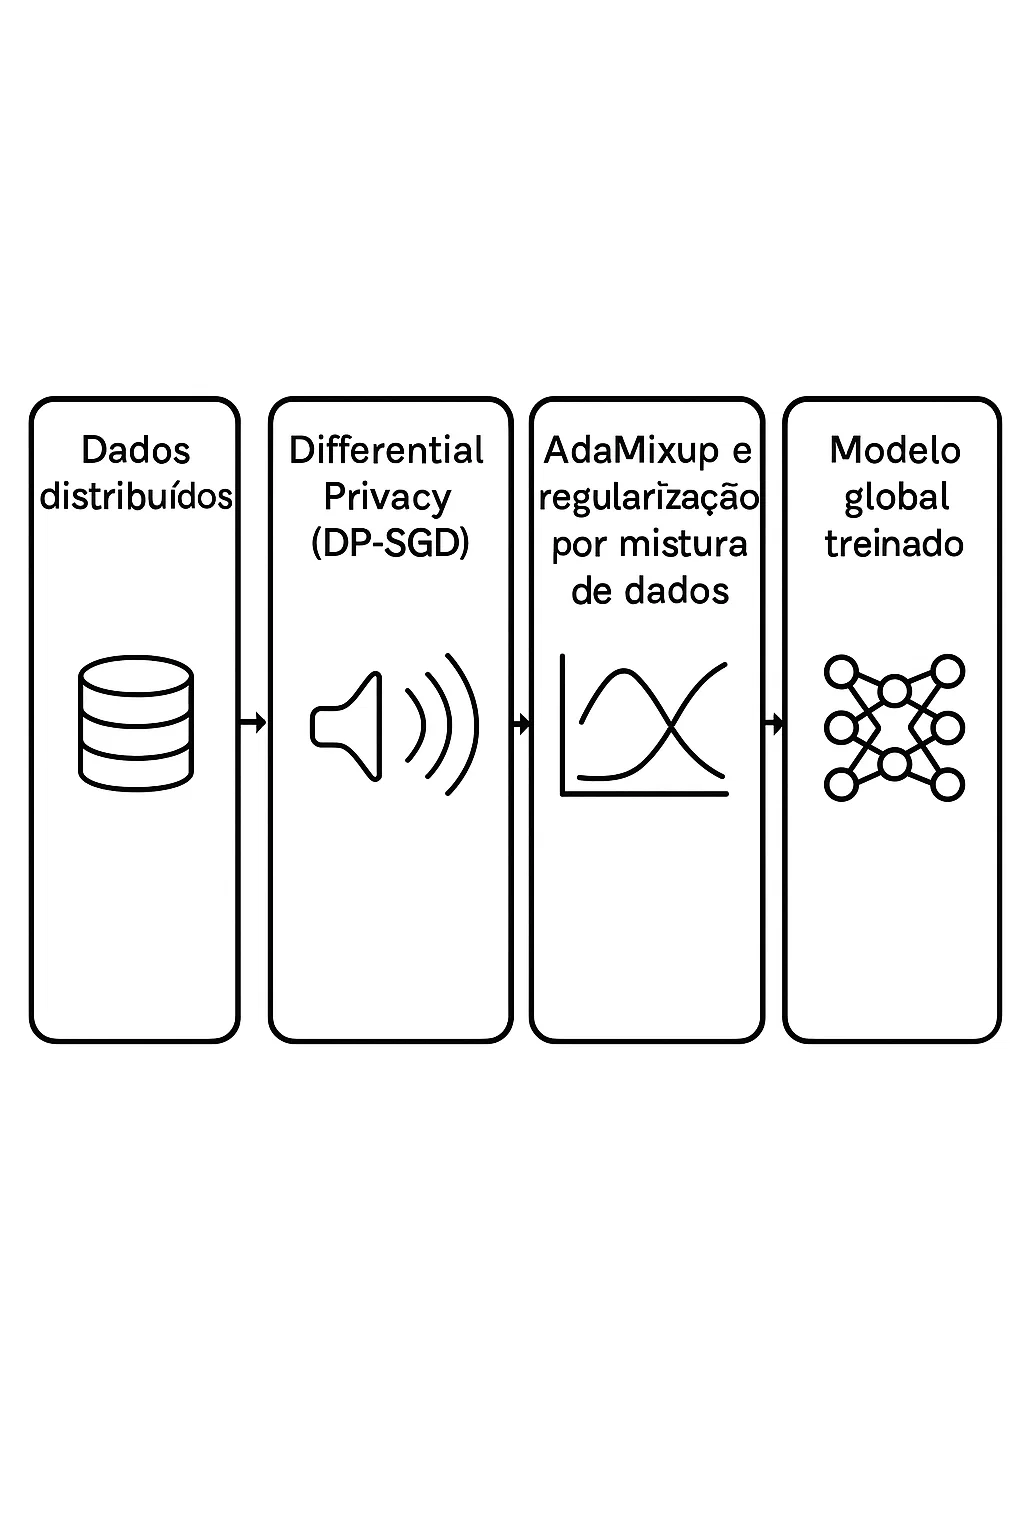
\includegraphics[width=0.4\linewidth]{Figura-10.png}
    \caption{\textit{Pipeline} conceitual de defesas híbridas em Fed-IDS. Combinação de DP-SGD, \textit{AdaMixup} e compressão de gradientes para mitigar ataques de inferência de pertencimento preservando a utilidade do modelo. Fonte: elaborado pela autora.}
    \label{fig:defesas_hibridas}
\end{figure}
Este capítulo apresentou a fundamentação teórica que sustenta a presente pesquisa, organizada em quatro eixos principais. Inicialmente, discutiu-se o \textit{Federated Learning}, destacando seus algoritmos fundacionais  como o FedAvg, o FedProx, o SCAFFOLD e o FedOpt  e enfatizando como a descentralização do treinamento visa conciliar eficiência e privacidade em cenários de dados distribuídos. Em seguida, abordaram-se os MIA, descrevendo seus conceitos, tipologias, avanços recentes, métricas de avaliação e implicações práticas, particularmente em ambientes \textit{white-box} e com dados heterogêneos, nos quais a vulnerabilidade é potencializada.

Nessa seção, explorou-se a evolução dos IDS e sua adaptação para ambientes federados. O Fed-IDS foi apresentado como uma abordagem promissora para lidar com os desafios de privacidade e escalabilidade em redes complexas, mas também como um alvo de novos riscos decorrentes da exposição a ataques de inferência. Trabalhos correlatos reforçam a relevância da integração entre FL e IDS, ao mesmo tempo em que apontam lacunas de pesquisa no que se refere à análise sistemática de vulnerabilidades a MIA nesse contexto.

Por fim, foram discutidas as principais estratégias de defesa, com ênfase em abordagens híbridas que combinam privacidade diferencial, regularização por mistura de dados e compressão de gradientes. Essas técnicas foram analisadas como alternativas viáveis para equilibrar os objetivos de privacidade e utilidade em Fed-IDS, embora tragam consigo desafios adicionais, como impacto em acurácia, custo computacional e calibragem de parâmetros de segurança.

De forma geral, este capítulo evidenciou que o Aprendizado Federado, apesar de ser uma ferramenta poderosa para cenários distribuídos e sensíveis, permanece suscetível a ataques de inferência de pertencimento, sobretudo em aplicações críticas como sistemas de detecção de intrusões. Essa constatação reforça a importância da investigação proposta nesta dissertação, que busca auditar a vulnerabilidade de Fed-IDS a MIA e avaliar a eficácia de defesas híbridas no equilíbrio entre privacidade, desempenho e custo. As próximas seções, dedicadas aos trabalhos recentes e à discussão de padrões em aberto, aprofundam essa análise, destacando as principais lacunas identificadas e os caminhos para a contribuição desta pesquisa.

\section{Trabalhos Recentes}
\label{sec:trabalhos_recentes}

O tema da privacidade em aprendizado de máquina, particularmente no contexto do \textit{Federated Learning}, tem atraído crescente atenção da comunidade científica. Nos últimos cinco anos, a literatura avançou em três direções principais:
\begin{enumerate}[label=(\Roman*)]
    \item Aprimoramento dos IDS tradicionais baseados em aprendizado de máquina;
    \item Integração do FL em sistemas de detecção de intrusões (Fed-IDS);
    \item Desenvolvimento de defesas híbridas contra ataques de inferência de pertencimento.
\end{enumerate}

Esta seção revisa trabalhos recentes em cada uma dessas frentes, destacando contribuições relevantes, tendências observadas e lacunas que motivam a presente pesquisa.

\subsection{Evolução dos IDS Tradicionais}
\label{subsec:evolucao_ids_tradicionais}

Os IDS baseados em aprendizado de máquina centralizado constituem a primeira geração de soluções que buscaram superar as limitações dos mecanismos tradicionais baseados apenas em assinaturas ou estatísticas manuais. A partir de 2020, observou-se um avanço expressivo em duas frentes principais: o uso de arquiteturas profundas, como redes convolucionais aplicadas à modelagem de tráfego \cite{tang2022fedids}, e a aplicação de técnicas de \textit{ensemble learning}, capazes de aumentar a robustez e a taxa de detecção em diferentes datasets \cite{lucas2023ensembleids}. 

Apesar desses avanços, tais abordagens mantêm a limitação estrutural da centralização: todos os dados de tráfego precisam ser coletados e processados em um único ponto. Essa característica, embora facilite o treinamento, gera riscos relevantes de privacidade e implica desafios de escalabilidade em redes modernas. Estudos recentes também evidenciam vulnerabilidades adicionais, como a possibilidade de reconstrução de dados a partir de gradientes em cenários centralizados \cite{yang2023deepleakage}, reforçando a exposição de informações sensíveis.

Além disso, revisões abrangentes demonstram que muitos trabalhos continuam baseados em datasets legados, como NSL-KDD, que já não refletem fielmente os padrões de tráfego contemporâneos \cite{lucas2023ensembleids}. Em contrapartida, pesquisas mais recentes começam a considerar ambientes emergentes, como redes 5G, mas ainda sob o paradigma centralizado \cite{alshammari2024springerids}. Por fim, levantamentos atuais reforçam que os IDS centralizados apresentam dificuldades de escalabilidade e falhas na preservação da privacidade, o que tem motivado a transição para abordagens federadas \cite{belenguer2025surveyfedids}.

Como se observa na Tabela~\ref{tab:ids_tradicionais_ano}, a produção recente migrou de
modelos clássicos para arquiteturas profundas e ensembles, mas preservando a centralização
de dados, o que evidencia limitações de privacidade e escalabilidade.

\begin{table}[H]
\centering
\footnotesize
\caption{Evolução dos IDS centralizados baseados em aprendizado de máquina (2020–2025).}
\label{tab:ids_tradicionais_ano}
\begin{tabularx}{\linewidth}{@{}p{2.2cm}p{1.0cm}p{3.0cm}p{2.5cm}X@{}}
\toprule
\textbf{Autor(es)} & \textbf{Ano} & \textbf{Técnica/Abordagem} & \textbf{Dataset(s)} & \textbf{Contribuições principais} \\ 
\midrule
Tang et al. \cite{tang2022fedids} & 2022 & CNN para modelagem de tráfego & CIC-IDS2017 & Uso de redes convolucionais para extrair padrões temporais; melhora significativa em TPR, mas mantém centralização de dados. \\
\addlinespace
Lucas et al. \cite{lucas2023ensembleids} & 2023 & Ensembles (Bagging, Boosting, Stacking) & NSL-KDD, CIC-IDS2017 & Revisão abrangente de técnicas de ensemble; ganhos consistentes em acurácia, mas limitações em datasets legados e interpretabilidade. \\
\addlinespace
Yang et al. \cite{yang2023deepleakage} & 2023 & Reconstrução de gradientes em IDS & CIC-IDS2017 & Explora ataques de \textit{deep leakage} para mostrar riscos em modelos centralizados; evidencia vulnerabilidades práticas. \\
\addlinespace
Alshammari et al. \cite{alshammari2024springerids} & 2024 & IDS centralizado em 5G/NGN & Tráfego 5G & Modelagem para redes de próxima geração; foco em latência e mobilidade; persiste a necessidade de centralização de dados. \\
\addlinespace
Belenguer et al. \cite{belenguer2025surveyfedids} & 2025 & Survey comparativo (centralizado vs federado) & CIC-IDS2017, UNSW-NB15 & Panorama atualizado até 2025; identifica que IDS centralizados não escalam bem e expõem riscos de privacidade, reforçando a transição para Fed-IDS. \\
\bottomrule
\end{tabularx}
\end{table}




\subsection{Integração de FL em IDS (Fed-IDS)}
\label{subsec:fed_ids}

A incorporação do \textit{Federated Learning} a sistemas de detecção de intrusões emerge como resposta direta às limitações do paradigma centralizado em cenários de redes distribuídas e sensíveis à privacidade. Em vez de consolidar tráfego de rede e metadados em um único repositório, o Fed-IDS permite que domínios administrativos distintos treinem modelos localmente e compartilhem apenas atualizações de parâmetros. Revisões sistemáticas recentes consolidam essa trajetória. Hernandez-Ramos et al. \cite{hernandez2023surveyfedids} apresentam um mapeamento do campo, evidenciando benefícios de privacidade e de escalabilidade, porém apontando desafios de heterogeneidade estatística, coordenação entre clientes e ausência de protocolos padronizados para avaliação de privacidade. Em perspectiva mais atualizada, Belenguer et al. \cite{belenguer2025surveyfedids} registram a predominância de datasets como CIC-IDS2017, UNSW-NB15 e Bot-IoT e reforçam a carência de auditorias explícitas a MIA no contexto de Fed-IDS.

No nível de propostas arquiteturais, a integração com tecnologias de confiança e trilhas de auditoria tem sido explorada para mitigar riscos do canal e de clientes maliciosos. Aouedi et al. \cite{aouedi2023blockchainids} propõem o F-BIDS, combinando FL com \textit{blockchain} para assegurar integridade e rastreabilidade das atualizações; Javeed et al. \cite{javeed2024zerotrust} avançam com o paradigma \textit{zero-trust}, reduzindo a dependência de pressupostos fortes sobre a benignidade dos participantes. Em paralelo, trabalhos voltados à operação prática do Fed-IDS enfrentam desafios de dinâmica de tráfego, mudança de conceito e recursos computacionais restritos: há investigações em \textit{continual learning} \cite{chetouane2025continualfedids}, transferência federada em borda \cite{raja2024transferfedids}, e arranjos específicos para IoT \cite{alshammari2024springerids,mazid2025flidpp,qiu2025fedaware}.

Quanto a mecanismos de privacidade no \textit{pipeline} federado de IDS, além de agregação segura, destacam-se abordagens que visam reduzir o \textit{leakage} em atualizações: esquemas de preservação de privacidade em detecção \cite{feng2023fedphp}, e estruturas explícitas para reforço de proteção de dados em cenários de intrusão \cite{saidi2025privacyfedids}. Ainda assim, a literatura carece de avaliações sistemáticas de MIA aplicadas a Fed-IDS, considerando simultaneamente: (i) a escolha do agregador (FedAvg, FedProx, SCAFFOLD, FedOpt), (ii) o grau de \textit{non-IID} entre clientes, e (iii) defesas híbridas (DP-SGD, regularizações de mistura e compressão de gradientes). Essa lacuna motiva a presente pesquisa, que propõe uma auditoria metodológica dos riscos de inferência de pertencimento em Fed-IDS, com quantificação do \textit{trade-off} entre privacidade, utilidade e custo.
A Tabela~\ref{tab:fed_ids_recentes} sintetiza resultados representativos de 2022–2025 em Fed-IDS,
com ênfase em arquiteturas, bases e contribuições.

% \vspace{0.5em}
% \noindent\textbf{Observação sobre datasets.} Em Fed-IDS, a avaliação experimental recorre majoritariamente a CIC-IDS2017 e UNSW-NB15, com crescimento de estudos em Bot-IoT e cenários SDN/edge. A padronização de protocolos que estratifiquem heterogeneidade, participação de clientes e métricas de privacidade permanece um ponto em aberto, já sinalizado por \cite{hernandez2023surveyfedids,belenguer2025surveyfedids}.
\begin{table}[H]
\centering
\footnotesize
\caption{Trabalhos recentes em Fed-IDS (2022–2025)}
\label{tab:fed_ids_recentes}
\begin{tabular}{p{3.2cm}p{1.2cm}p{3.0cm}p{2.8cm}p{5.0cm}}
\toprule
\textbf{Autor(es)} & \textbf{Ano} & \textbf{Cenário/Arquitetura} & \textbf{Base de dados} & \textbf{Principais contribuições} \\
\midrule
Hernandez-Ramos et al. \cite{hernandez2023surveyfedids} & 2023 & Revisão sistemática de Fed-IDS & CIC-IDS2017, UNSW-NB15, Bot-IoT & Síntese do estado da arte; benefícios de privacidade e escalabilidade; aponta ausência de protocolos padronizados para avaliação de privacidade. \\
Aouedi et al. \cite{aouedi2023blockchainids} & 2023 & F-BIDS (FL com Blockchain) & IoT & Integração de blockchain ao FL; assegura integridade e rastreabilidade das atualizações. \\
Javeed et al. \cite{javeed2024zerotrust} & 2024 & Arquitetura Zero-Trust & CIC-IDS2017, Edge-IIoT & Mitigação de clientes maliciosos; reforço de autenticação e controle de acesso. \\
Belenguer et al. \cite{belenguer2025surveyfedids} & 2025 & Revisão atualizada de Fed-IDS & CIC-IDS2017, UNSW-NB15 & Panorama até 2025; destaca carência de auditorias explícitas de ataques de inferência de pertencimento (MIA). \\
Tang et al. \cite{tang2022fedids} & 2022 & IDS federado com aprendizado profundo & CIC-IDS2017 & Demonstra viabilidade do FL em detecção de intrusões mantendo dados distribuídos. \\
Feng et al. \cite{feng2023fedphp} & 2023 & FedPHP (FL preservando privacidade) & Tráfego de rede (AISec) & Proposta de preservação de privacidade no \textit{pipeline} de IDS federado. \\
Alshammari et al. \cite{alshammari2024springerids} & 2024 & Fed-IDS em redes 5G & Cenários de borda/5G & Adaptação do FL a ambientes móveis; análise de latência e mobilidade. \\
Chetouane et al. \cite{chetouane2025continualfedids} & 2025 & Fed-IDS com aprendizado contínuo & SDN & Tratamento de mudanças de conceito em tráfego dinâmico. \\
Mazid et al. \cite{mazid2025flidpp} & 2025 & FL proativo para IoT & IoT & Reconhecimento proativo de intrusões; foco em restrições de energia e comunicação. \\
Raja et al. \cite{raja2024transferfedids} & 2024 & Transferência federada & Edge datasets & Melhora da generalização entre ambientes heterogêneos de borda. \\
Qiu et al. \cite{qiu2025fedaware} & 2025 & FedAware (IoT e nuvem) & IoT/Cloud & Coordenação distribuída em cenários IoT; foco em heterogeneidade de dispositivos. \\
Saidi et al. \cite{saidi2025privacyfedids} & 2025 & Fed-IDS com foco em privacidade & UNSW-NB15 & Estratégias explícitas de preservação de privacidade; análise do trade-off entre utilidade e custo. \\
\bottomrule
\end{tabular}
\\[0.5em]
% \raggedright \textbf{Fonte:} Elaborado pela autora com base em Hernandez-Ramos et al. (2023), Aouedi et al. (2023), Javeed et al. (2024), Belenguer et al. (2025), Tang et al. (2022), Feng et al. (2023), Alshammari et al. (2024), Chetouane et al. (2025), Mazid et al. (2025), Raja et al. (2024), Qiu et al. (2025) e Saidi et al. (2025).
\end{table}



\subsection{Ataques de \textit{Membership Inference} e implicações para Fed-IDS}

O problema dos MIA ganhou notoriedade a partir do trabalho seminal de Shokri et al. \cite{shokri2017mia}, que demonstrou a vulnerabilidade de modelos supervisionados em cenários \textit{black-box}. Avanços posteriores, como os de Yeom et al. \cite{yeom2018privacyrisk}, estabeleceram a relação direta entre \textit{overfitting} e risco de privacidade, enquanto Nasr et al. \cite{nasr2019comprehensive} expandiram a análise para cenários \textit{white-box}, introduzindo ataques passivos e ativos em ambientes centralizados e federados. Mais recentemente, Carlini et al. \cite{carlini2022firstprinciples} formalizaram os MIA a partir de princípios estatísticos fundamentais, e Liu et al. \cite{liu2022trajectory} mostraram que a trajetória da função de perda (\textit{loss trajectory}) é uma fonte adicional de sinal para inferência. Revisões como a de Bai et al. \cite{bai2024survey} consolidam essas descobertas, evidenciando a maturidade e a diversidade do campo.

No entanto, apesar da extensa literatura sobre MIA, poucos estudos avaliaram sistematicamente a vulnerabilidade de Fed-IDS a esse tipo de ataque. Esse hiato torna-se ainda mais preocupante considerando-se que, em cenários federados, adversários podem explorar atualizações de gradientes e parâmetros locais, ampliando a superfície de ataque \cite{nasr2019comprehensive}. 
A Tabela~\ref{tab:defesas_mia} organiza os principais mecanismos de defesa empregados entre 2016 e 2025.
\begin{table}[H]
\centering
\footnotesize
\caption{Principais trabalhos sobre Membership Inference Attacks (MIA) e suas implicações para Aprendizado Federado e Fed-IDS}
\label{tab:mia_fedids}
\begin{tabular}{p{3.2cm}p{1.2cm}p{2.8cm}p{2.8cm}p{5.2cm}}
\toprule
\textbf{Autor(es)} & \textbf{Ano} & \textbf{Cenário} & \textbf{Tipo de ataque} & \textbf{Principais contribuições} \\
\midrule
Shokri et al. \cite{shokri2017mia} & 2017 & Modelos supervisionados & \textit{Black-box} & Trabalho seminal; introduz ataques de inferência de pertencimento baseados em modelos sombra. \\
Yeom et al. \cite{yeom2018privacyrisk} & 2018 & Modelos supervisionados & \textit{Black-box} & Relaciona risco de privacidade ao sobreajuste; propõe métrica de \textit{advantage}. \\
Nasr et al. \cite{nasr2019comprehensive} & 2019 & Ambientes centralizados e federados & \textit{White-box} (passivo e ativo) & Analisa ataques em cenários centralizados e federados; amplia a superfície de ataque explorando gradientes. \\
Carlini et al. \cite{carlini2022firstprinciples} & 2022 & Modelos de classificação supervisionada & Formalização estatística & Reexamina pressupostos anteriores e propõe formulação estatística robusta de MIA. \\
Liu et al. \cite{liu2022trajectory} & 2022 & Aprendizado supervisionado & \textit{Loss trajectory} & Demonstra que a evolução temporal da função de perda fornece sinal informativo adicional para inferência. \\
Bai et al. \cite{bai2024survey} & 2024 & Aprendizado federado & Revisão & Consolida descobertas recentes; sintetiza ataques, defesas e lacunas ainda existentes no contexto de FL. \\
Nikolaidis et al. \cite{nikolaidis2025studyfl} & 2025 & Aprendizado federado & Estudo sistemático & Análise abrangente dos MIA em FL; compara diferentes métodos, métricas e discute cenários emergentes (IoT, edge, RAG). \\
\bottomrule
\end{tabular}
\\[0.5em]
% \raggedright \textbf{Fonte:} Elaborado pela autora com base em Shokri et al. (2017), Yeom et al. (2018), Nasr et al. (2019), Carlini et al. (2022), Liu et al. (2022), Bai et al. (2024) e Nikolaidis et al. (2025).
\end{table}

\subsection{Defesas Híbridas e Estratégias de Mitigação}
\label{subsec:defesas_hibridas}

Para enfrentar os riscos de privacidade em FL, múltiplas linhas de defesa têm sido propostas. A privacidade diferencial, introduzida por Abadi et al. \cite{abadi2016dpsgd}, consolidou-se como um dos mecanismos mais relevantes, embora trabalhos como o de Bagdasaryan e Shmatikov \cite{bagdasaryan2019dpimpact} tenham demonstrado seus impactos adversos na acurácia de modelos heterogêneos. Paralelamente, técnicas baseadas em mistura de dados, como o AdaMixup, e métodos de compressão de gradientes surgem como alternativas promissoras. Li et al. \cite{li2023gradientpruning} exploraram a poda adaptativa de gradientes com privacidade, enquanto Wu et al. \cite{wu2023pruningfl} e Wei et al. \cite{wei2024gradientsparsification} mostraram que a compressão pode reduzir tanto o custo de comunicação quanto a vulnerabilidade a ataques. 

Essas abordagens, ainda que eficazes de forma isolada, apontam para a necessidade de defesas híbridas capazes de integrar mecanismos distintos, conciliando preservação de privacidade, robustez contra ataques e manutenção da utilidade do modelo.



\begin{table}[H]
\centering
\footnotesize
\caption{Principais defesas contra Membership Inference Attacks (MIA) em Aprendizado Federado (2016–2025).}
\label{tab:defesas_mia}
\begin{tabular}{p{3.2cm}p{1.2cm}p{3.0cm}p{6.2cm}}
\toprule
\textbf{Autor(es)} & \textbf{Ano} & \textbf{Mecanismo} & \textbf{Principais contribuições} \\
\midrule
Abadi et al. \cite{abadi2016dpsgd} & 2016 & DP-SGD & Introduzem treinamento com privacidade diferencial em redes neurais profundas; marco inicial para defesa em ML. \\
Bagdasaryan \& Shmatikov \cite{bagdasaryan2019dpimpact} & 2019 & DP em FL & Demonstram que a DP pode impactar desigualmente clientes em cenários heterogêneos, comprometendo acurácia. \\
Li et al. \cite{li2023gradientpruning} & 2023 & Poda de gradientes + DP & Combina pruning adaptativo e privacidade diferencial; melhora eficiência de comunicação e preserva privacidade. \\
Wu et al. \cite{wu2023pruningfl} & 2023 & Compressão de modelos & Explora pruning para reduzir custos de comunicação em FL e mitigar risco de vazamento. \\
Wei et al. \cite{wei2024gradientsparsification} & 2024 & Sparsificação de gradientes & Propõe gradiente esparso com DP para eficiência em redes sem fio; reduz vulnerabilidade a MIA. \\
Yin et al. \cite{yin2024miafl} & 2024 & Agregação confiável & Estratégia de agregação robusta para reduzir inferência de membros em FL; melhora segurança em clientes heterogêneos. \\
Ni et al. \cite{niu2025dualdefense} & 2025 & Defesa dual  & Combina exclusão preemptiva de amostras de alto risco com distilação de conhecimento para mitigar MIA. \\
\bottomrule
\end{tabular}
\\[0.5em]
% \raggedright \textbf{Fonte:} Elaborado pela autora com base em Abadi et al. (2016), Bagdasaryan \& Shmatikov (2019), Li et al. (2023), Wu et al. (2023), Wei et al. (2024), Yin et al. (2024) e Ni et al. (2025).
\end{table}


% \subsection{Síntese Crítica}

% A revisão dos trabalhos recentes permite identificar tendências claras: (i) a evolução dos IDS de arquiteturas centralizadas para modelos federados; (ii) a consolidação dos MIA como ameaça concreta e amplamente estudada em aprendizado de máquina; e (iii) o surgimento de defesas híbridas como caminho viável para equilibrar privacidade e utilidade. Ao mesmo tempo, evidencia lacunas importantes: (a) a escassez de estudos que avaliem de forma integrada ataques de inferência em Fed-IDS; (b) a ausência de protocolos padronizados para medir privacidade em cenários federados; e (c) a necessidade de explorar defesas compostas, que combinem técnicas como DP-SGD, AdaMixup e compressão de gradientes.




\section{Discussões e Padrões em Aberto}
\label{sec:discussoes_aberto}

A revisão conduzida nos capítulos anteriores evidenciou avanços relevantes em IDS, \textit{Federated Learning} e ataques de inferência de pertencimento, além de um conjunto diversificado de estratégias de mitigação. Contudo, ao analisar criticamente a literatura, emergem lacunas estruturais e padrões recorrentes que limitam a consolidação de soluções práticas, seguras e escaláveis. Este capítulo organiza tais questões em eixos temáticos, de forma a delinear os principais desafios em aberto que a proposta metodológica desta dissertação busca endereçar.

\subsection{Heterogeneidade de Dados e Robustez de Modelos}
Grande parte dos estudos em FL, incluindo cenários de Fed-IDS, ainda se baseia em pressupostos simplificados de distribuição dos dados. A predominância de cenários \textit{IID} ignora a realidade de ambientes distribuídos, como redes IoT e arquiteturas de borda, onde o fenômeno \textit{non-IID} é regra e não exceção. Embora algoritmos como FedProx \cite{li2020fedprox} e SCAFFOLD \cite{karimireddy2020scaffold} avancem na mitigação do \textit{client drift}, permanece em aberto o desafio de garantir estabilidade e desempenho sob condições de alta heterogeneidade estatística. Isso é particularmente crítico em IDS, nos quais padrões de tráfego variam de forma dinâmica e adversarial.

\subsection{Superfície de Ataque Ampliada em Fed-IDS}
A literatura recente reconhece que o paradigma federado expande a superfície de ataque ao expor gradientes, parâmetros locais e metadados de comunicação. Estudos como os de Nasr et al. \cite{nasr2019comprehensive} demonstram que ataques \textit{white-box}, passivos ou ativos, exploram diretamente tais sinais. Entretanto, poucos trabalhos aplicam auditorias sistemáticas a Fed-IDS, sobretudo considerando a especificidade de tráfego de rede e a variação de clientes em cada rodada. Essa ausência de benchmarks de segurança específicos para Fed-IDS constitui uma lacuna crítica, limitando a avaliação comparativa de riscos.

\subsection{Protocolos Experimentais Fragmentados}
Outro padrão identificado é a ausência de protocolos experimentais padronizados. Há forte dependência de datasets legados, como CIC-IDS2017 e UNSW-NB15, os quais, apesar de úteis, já não refletem integralmente a complexidade de tráfego em redes modernas. Revisões recentes \cite{belenguer2025surveyfedids} destacam a carência de protocolos que estratifiquem resultados de forma consistente segundo fatores como:
\begin{enumerate}[label=(\alph*)]
    \item grau de heterogeneidade dos dados locais;
    \item frequência e participação dos clientes em cada rodada;
    \item escolha do algoritmo de agregação (FedAvg, FedProx, SCAFFOLD, FedOpt);
    \item métricas de privacidade e de utilidade avaliadas em conjunto.
\end{enumerate}
Sem essa padronização, comparações entre propostas tornam-se incompletas e a evolução do campo perde em cumulatividade científica.

\subsection{Limitações das Defesas Isoladas}
As defesas existentes contra MIA no contexto federado concentram-se em mecanismos isolados, como privacidade diferencial \cite{abadi2016dpsgd}, compressão de gradientes \cite{wu2023pruningfl,wei2024gradientsparsification} ou agregações robustas \cite{yin2024miafl}. Ainda que eficazes em cenários específicos, tais técnicas apresentam limitações significativas:
\begin{itemize}
    \item a privacidade diferencial impõe perdas de acurácia, particularmente em cenários de dados heterogêneos \cite{bagdasaryan2019dpimpact};
    \item métodos de compressão reduzem custos de comunicação, mas podem comprometer a convergência;
    \item regularizações baseadas em mistura de dados ainda carecem de validações empíricas amplas.
\end{itemize}
Esse quadro sugere a necessidade de abordagens híbridas que combinem diferentes mecanismos, conciliando robustez, privacidade e utilidade em Fed-IDS.

\subsection{Carência de Auditorias sobre Impacto Prático}
Apesar da riqueza teórica e experimental, observa-se escassez de estudos que avaliem os impactos práticos de ataques e defesas em cenários reais. Poucos trabalhos investigam o custo computacional, energético e de comunicação associados à aplicação simultânea de defesas em ambientes IoT ou SDN. Da mesma forma, há lacunas quanto ao impacto regulatório e ético da exposição a ataques de inferência, especialmente em setores críticos como saúde e finanças. Esses aspectos precisam ser incorporados a futuros protocolos experimentais para que os resultados extrapolem o campo acadêmico e se tornem aplicáveis na prática.

\subsection{Síntese das Lacunas e Oportunidades}
Além dos desafios já descritos, destacam-se duas lacunas estruturais que esta pesquisa pretende abordar futuramente. A primeira refere-se à \textbf{escassez de benchmarks padronizados para avaliação de Fed-IDS}, o que limita a comparabilidade entre estudos e impede a construção de métricas reprodutíveis de vulnerabilidade e mitigação. A ausência de um repositório público que contemple cenários heterogêneos e adversariais específicos de detecção de intrusões federadas dificulta a validação empírica e o avanço cumulativo do campo. A segunda lacuna diz respeito à \textbf{inexistência de métricas padronizadas de privacidade em Aprendizado Federado}. Atualmente, os estudos empregam métricas distintas, como \textit{advantage}, AUC-ROC, ou TPR@FPR, sem consenso sobre qual quantifica de forma mais fidedigna o risco de inferência. Essa falta de uniformização torna a comparação entre defesas imprecisa e compromete a definição de parâmetros mínimos de segurança. A consolidação de benchmarks e métricas de privacidade unificadas representa, portanto, um passo essencial para a maturidade científica e prática de sistemas Fed-IDS.

A Tabela~\ref{tab:discussoes_aberto} sintetiza os principais padrões em aberto identificados, relacionando-os a potenciais direções de pesquisa. Esse mapeamento serve como base para a formulação da proposta metodológica desenvolvida no próximo capítulo.

\begin{table}[H]
\centering
\footnotesize
\caption{Síntese dos padrões em aberto e oportunidades de pesquisa em Fed-IDS.}
\label{tab:discussoes_aberto}
\begin{tabular}{p{3.5cm}p{6.5cm}p{5.0cm}}
\toprule
\textbf{Eixo} & \textbf{Padrão em aberto} & \textbf{Oportunidade de pesquisa} \\
\midrule
Heterogeneidade de dados & Algoritmos ainda frágeis em cenários altamente \textit{non-IID} & Desenvolvimento de agregadores adaptativos e defesas sensíveis à heterogeneidade \\
Superfície de ataque & Ausência de benchmarks específicos para Fed-IDS & Proposta de auditorias sistemáticas de MIA em IDS federados \\
Protocolos experimentais & Fragmentação de datasets e métricas & Criação de protocolos padronizados que integrem privacidade, utilidade e custo \\
Defesas isoladas & Limitações de DP, compressão ou regularizações quando aplicadas separadamente & Integração de defesas híbridas em \textit{pipelines} práticos de Fed-IDS \\
Impacto prático & Poucos estudos sobre custo energético, computacional e ético & Avaliação multidimensional em cenários IoT, edge e setores críticos \\
\bottomrule
\end{tabular}
\end{table}

\begin{figure}[H]
    \centering
    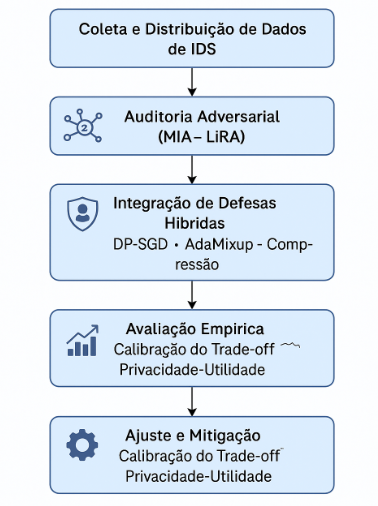
\includegraphics[width=0.5\linewidth]{Figura-12.png}
    \caption{\textit{Pipeline} conceitual da Auditoria e Mitigação em Fed-IDS. O \textit{framework} proposto integra cinco estágios principais: (1) coleta e distribuição de dados de IDS; (2) auditoria adversarial por ataques de inferência de pertencimento (LiRA e variantes); (3) integração de defesas híbridas, como DP-SGD, \textit{AdaMixup} e compressão de gradientes; (4) avaliação empírica e calibração do \textit{trade-off} privacidade-utilidade; e (5) ajustes iterativos para mitigação e estabilidade do modelo. Fonte: elaborado pela autora.}
    \label{fig:pipeline_fedids}
\end{figure}

A Figura \ref{fig:pipeline_fedids} sintetiza o fluxo conceitual da proposta deste trabalho, representando a transição entre auditoria, defesa e mitigação. O \textit{pipeline} reflete o objetivo central de estabelecer uma metodologia sistemática para avaliar e reduzir riscos de inferência de pertencimento em sistemas Fed-IDS, mantendo o equilíbrio entre privacidade e desempenho. Essa visão integradora reforça a contribuição prática e científica do estudo, consolidando um arcabouço que pode ser adaptado a diferentes arquiteturas de aprendizado federado.

Em suma, o campo de Fed-IDS encontra-se em um ponto de inflexão: há avanços sólidos em algoritmos, ataques e defesas, mas a ausência de padronização e a carência de auditorias sistemáticas limitam sua maturidade. O próximo capítulo desta dissertação apresenta a proposta metodológica que busca responder a parte dessas lacunas, estruturando um protocolo experimental de auditoria de ataques de inferência de pertencimento em Fed-IDS.


\chapter{Metodologia}
\label{sec:auditoria_llm}

Como contribuição preliminar desta dissertação, foi desenvolvido e submetido um \textit{framework} de auditoria multidimensional de privacidade aplicado a modelos de linguagem de grande escala (\textit{Large Language Models}, LLMs), publicado como artigo nos anais do CIARP 2026 (Pontara et al., 2026). Embora o foco principal desta dissertação seja a auditoria de Fed-IDS, o trabalho em LLMs valida a abordagem metodológica proposta e demonstra sua aplicabilidade em contextos complementares de aprendizado de máquina. A metodologia e os resultados apresentados neste capítulo fornecem subsídios diretos para a transposição do arcabouço de auditoria ao cenário federado de detecção de intrusões.

\section{Motivação e Contextualização}

Os modelos de linguagem treinados em grandes volumes de texto podem memorizar exemplos específicos do conjunto de treinamento, criando riscos concretos de privacidade~\cite{carlini2019secret}. Os ataques de inferência de pertencimento exploram esse comportamento para determinar se uma amostra foi utilizada durante o treinamento, constituindo uma ferramenta fundamental para auditoria de privacidade. Apesar dos avanços recentes, os protocolos de avaliação de MIA permanecem limitados em três aspectos: (i) dependência de métricas agregadas como AUC, que não indicam quais amostras são detectadas; (ii) avaliação de um único ataque em configuração restrita de modelo e \textit{dataset}; e (iii) ausência de quantificação da diversidade de detecção e da estabilidade das predições.

\section{Arcabouço de Auditoria Multidimensional}
\label{sec:framework_auditoria}

O arcabouço proposto formula a auditoria de privacidade como um processo de avaliação multidimensional que analisa ataques de inferência de pertencimento além do desempenho agregado de discriminação. Dado um modelo alvo $M_\theta$, um conjunto de dados candidato $\mathcal{D}$ e uma família de ataques $\mathcal{F}$, o \textit{framework} avalia cinco dimensões complementares de exposição à privacidade:

\begin{enumerate}[label=(\roman*)]
    \item \textbf{Discriminação}: mede a capacidade de distinguir membros de não membros utilizando métricas como AUC, precisão, \textit{recall} e F1-\textit{score}.
    \item \textbf{Cobertura}: mede a amplitude com que os ataques identificam amostras vulneráveis. Dois ataques podem alcançar desempenho de discriminação semelhante enquanto expõem subconjuntos substancialmente diferentes dos dados de treinamento.
    \item \textbf{Estabilidade}: mede a consistência das predições em avaliações repetidas, utilizando a similaridade de Jaccard entre conjuntos de membros detectados.
    \item \textbf{Sensibilidade}: mede como o desempenho do ataque varia conforme as condições experimentais, incluindo arquitetura do modelo, domínio do \textit{dataset} e nível de repetição de \textit{canaries}.
    \item \textbf{Vulnerabilidade}: caracteriza quais amostras individuais são mais suscetíveis à exposição com base em propriedades textuais como raridade de \textit{tokens}, comprimento do texto e diferença de \textit{loss}.
\end{enumerate}

Essas dimensões proporcionam uma caracterização mais abrangente do vazamento de pertencimento do que métricas de discriminação agregadas isoladamente. O arcabouço avalia não apenas se os ataques são precisos, mas também se identificam as mesmas amostras vulneráveis, se permanecem estáveis entre execuções e se se comportam de forma consistente sob diferentes condições experimentais.

\section{Estratégias de Ataque Avaliadas}

Foram avaliadas seis estratégias de ataque, cada uma explorando características estatísticas distintas associadas à memorização:

\begin{enumerate}[label=(\roman*)]
    \item \textbf{Ataque baseado em \textit{loss}}: utiliza a entropia cruzada negativa como \textit{score} de pertencimento:
    \begin{equation}
    s_{\mathrm{loss}}(x) = \frac{1}{T-1}\sum_{t=2}^{T} \log P_{M_\theta}(x_t \mid x_{<t})
    \end{equation}
    onde $x_t$ denota o \textit{token} na posição $t$ e $P_{M_\theta}(x_t \mid x_{<t})$ é a probabilidade condicional atribuída pelo modelo alvo.

    \item \textbf{\textit{Reference-gap}}: compara o modelo alvo com um modelo de referência pré-treinado:
    \begin{equation}
    s_{\mathrm{ref}}(x) = \ell_{M_\theta}(x) - \ell_{M_{\mathrm{ref}}}(x)
    \end{equation}
    onde $\ell_M(x)$ denota a \textit{log-likelihood} média por \textit{token} atribuída pelo modelo $M$.

    \item \textbf{Min-K\%}: calcula a média das $k$ menores \textit{log-probabilidades} de \textit{tokens}, incorporando perturbação de vizinhança sobre $V=3$ variantes textuais.

    \item \textbf{Min-K\%++}: aplica normalização por \textit{z-score}:
    \begin{equation}
    z_t = \frac{\ell_t - \mu_\ell}{\sigma_\ell}
    \end{equation}
    onde $\ell_t$ denota a \textit{log-probabilidade} do \textit{token} $x_t$, e $\mu_\ell$ e $\sigma_\ell$ correspondem à média e ao desvio padrão das \textit{log-probabilidades} na sequência.

    \item \textbf{ReCaLL}: estima pertencimento por meio de \textit{log-likelihood} condicional relativa entre modelos alvo e de referência~\cite{xie2024recall}:
    \begin{equation}
    s_{\mathrm{recall}}(x) = \ell_{M_\theta}(x) - \ell_{M_{\mathrm{ref}}}(x)
    \end{equation}

    \item \textbf{LiRA}: computa um \textit{z-score} da \textit{loss} do modelo alvo contra distribuições de \textit{shadow models}~\cite{carlini2022firstprinciples}:
    \begin{equation}
    s_{\mathrm{lira}}(x) = -\frac{\mathrm{loss}_{M_\theta}(x) - \mu_{\mathrm{shadow}}(x)}{\sigma_{\mathrm{shadow}}(x)}
    \end{equation}
    onde $\mu_{\mathrm{shadow}}$ e $\sigma_{\mathrm{shadow}}$ são estimados a partir das \textit{losses} dos \textit{shadow models}.
\end{enumerate}

\section{Configuração Experimental}

A avaliação foi conduzida sobre quatro modelos de linguagem: DistilGPT-2 (82M parâmetros), GPT-2 (124M), Pythia-160M (160M, EleutherAI) e OPT-125M (125M, Meta). Todos os modelos foram ajustados com taxa de aprendizado $5\times10^{-5}$, tamanho de \textit{batch} 4, duas épocas, comprimento de sequência 128, otimizador AdamW com decaimento de peso $10^{-2}$ e 10\% de \textit{warmup}.

Os \textit{datasets} utilizados foram WikiText-2 ($\sim$2M \textit{tokens}), WikiText-103 ($\sim$103M \textit{tokens}) e OpenWebText (domínio web), com 4.000 textos de treinamento e 800 de avaliação por corpus.

Para inserção de \textit{canaries}, foram utilizadas $n=25$ sequências sintéticas por \textit{dataset}, repetidas $r \in \{1, 2, 4, 8\}$ vezes, seguindo a metodologia de Carlini et al. (2019). A matriz experimental combina quatro modelos, três \textit{datasets} e quatro níveis de repetição, resultando em 48 configurações experimentais distintas e 288 avaliações de ataque.

\begin{figure}[H]
    \centering
    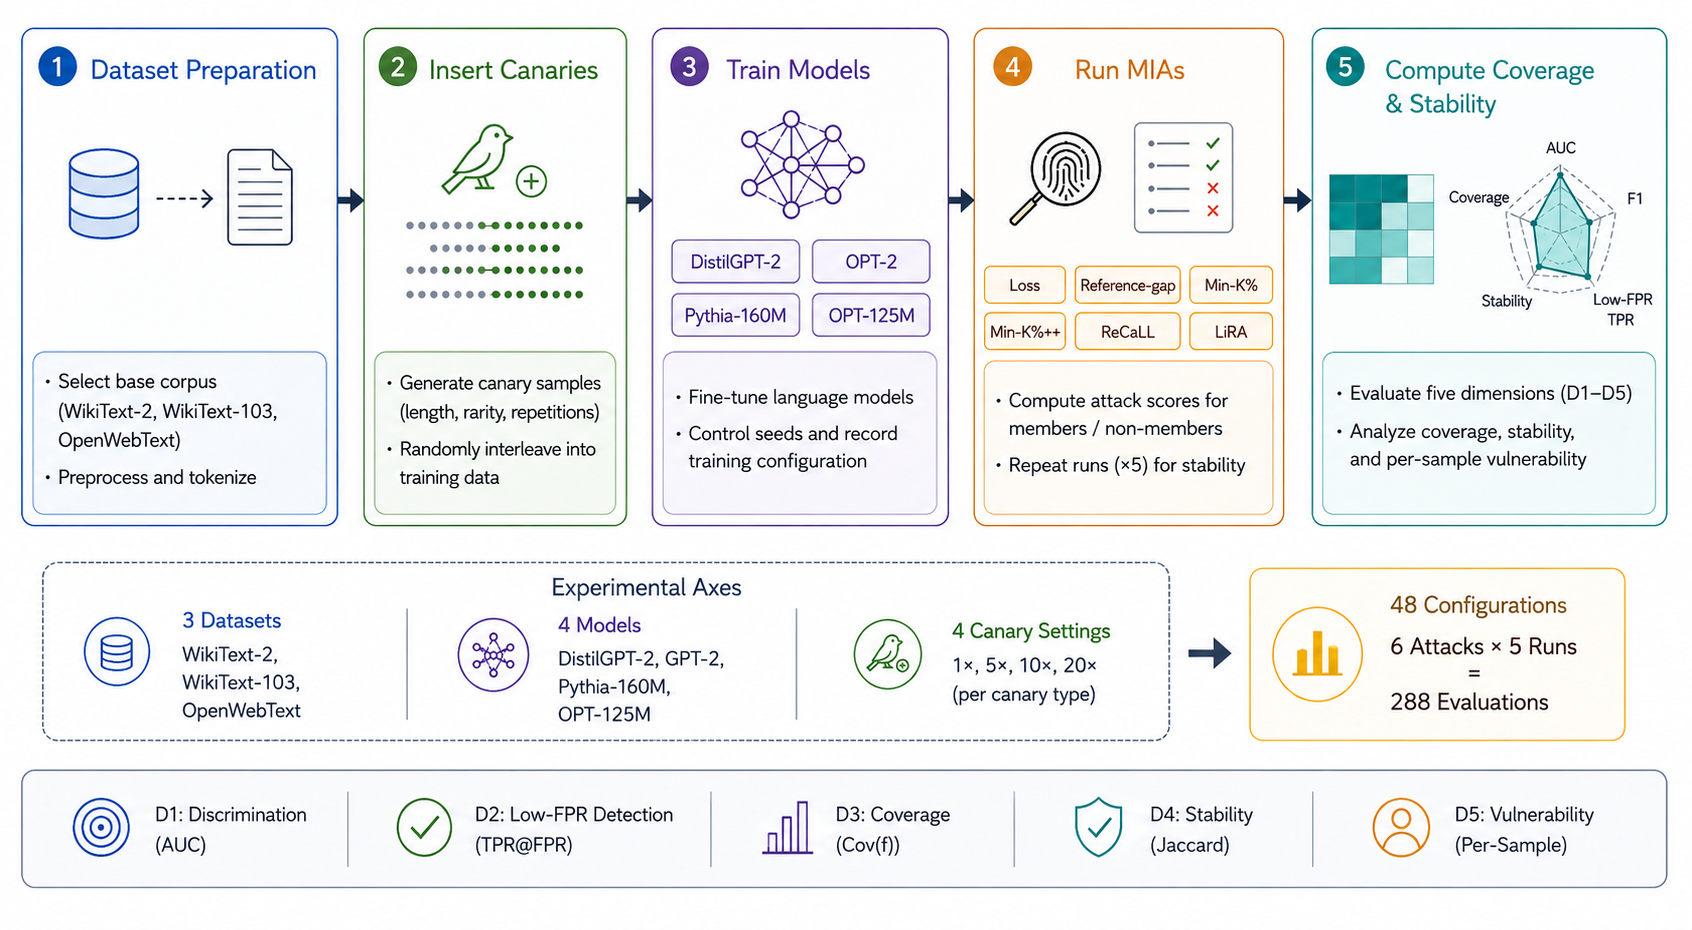
\includegraphics[width=0.85\linewidth]{fig-1-pipeline.png}
    \caption{\textit{Pipeline} de auditoria multidimensional proposto. O arcabouço orquestra 48 experimentos envolvendo quatro modelos, três \textit{datasets} e quatro níveis de repetição de \textit{canaries}. Fonte: elaborado pela autora.}
    \label{fig:pipeline_ciarp}
\end{figure}

\chapter{Resultados Parciais}
\label{sec:resultados_parciais}

Este capítulo reúne os resultados parciais obtidos com a validação do arcabouço de auditoria multidimensional em modelos de linguagem, discute suas implicações para a auditoria de Fed-IDS e consolida as conclusões parciais, os próximos passos e o cronograma da pesquisa.

\section{Resultados Experimentais}

\subsection{Desempenho Agregado dos Ataques}

A Tabela~\ref{tab:aggregate_ciarp} apresenta o desempenho médio de todos os ataques nas 48 configurações experimentais.

\begin{table}[H]
\centering
\caption{Desempenho agregado dos ataques nas 48 configurações experimentais.}
\label{tab:aggregate_ciarp}
\begin{tabular}{lcccc}
\toprule
\textbf{Ataque} & \textbf{AUC} & \textbf{F1} & \textbf{TPR@1\%} & \textbf{TPR@5\%} \\
\midrule
\textit{Loss}       & 0,816$\pm$0,085 & 0,801 & 0,129 & 0,278 \\
\textit{Ref-gap}    & 0,842$\pm$0,082 & 0,851 & 0,202 & 0,303 \\
Min-K\%    & 0,816$\pm$0,076 & 0,789 & 0,131 & 0,303 \\
Min-K\%++  & 0,646$\pm$0,069 & 0,690 & 0,037 & 0,121 \\
ReCaLL     & 0,867$\pm$0,071 & 0,866 & 0,204 & 0,336 \\
LiRA       & 0,791$\pm$0,164 & 0,809 & 0,146 & 0,268 \\
\bottomrule
\end{tabular}
\end{table}

O ReCaLL alcançou a maior AUC média (0,867), seguido pelo \textit{reference-gap} (0,842), indicando a superioridade de ataques baseados em referência nos cenários de \textit{fine-tuning} avaliados. Em contraste, o Min-K\%++ obteve a menor AUC (0,646), enquanto o LiRA exibiu a maior variabilidade ($\pm$0,164). A análise estatística confirmou que o ReCaLL superou significativamente todos os demais ataques ($p < 0,001$, correção de Bonferroni).

\subsection{Análise por Modelo}

A Tabela~\ref{tab:model_ciarp} reporta a AUC média obtida por cada ataque nos modelos avaliados.

\begin{table}[H]
\centering
\caption{AUC média por ataque e modelo de linguagem.}
\label{tab:model_ciarp}
\begin{tabular}{lcccccc}
\toprule
\textbf{Modelo} & \textbf{\textit{Loss}} & \textbf{\textit{Ref}} & \textbf{MK} & \textbf{MK++} & \textbf{ReC} & \textbf{LiRA} \\
\midrule
DistilGPT-2 & 0,720 & 0,826 & 0,738 & 0,588 & 0,846 & 0,834 \\
GPT-2       & 0,739 & 0,820 & 0,750 & 0,591 & 0,843 & 0,838 \\
Pythia-160M & 0,928 & 0,875 & 0,919 & 0,710 & 0,903 & 0,911 \\
OPT-125M    & 0,856 & 0,852 & 0,846 & 0,691 & 0,879 & 0,576 \\
\bottomrule
\end{tabular}
\end{table}

O Pythia-160M demonstrou consistentemente a maior vulnerabilidade de pertencimento (AUC de até 0,928), indicando que o \textit{design} do \textit{tokenizer}, a composição do corpus de pré-treinamento e características arquiteturais influenciam conjuntamente os padrões de memorização. O OPT-125M exibiu comportamento anômalo com LiRA (0,576), provavelmente associado a distribuições de \textit{shadow models} com baixa variância.

\begin{figure}[H]
\centering
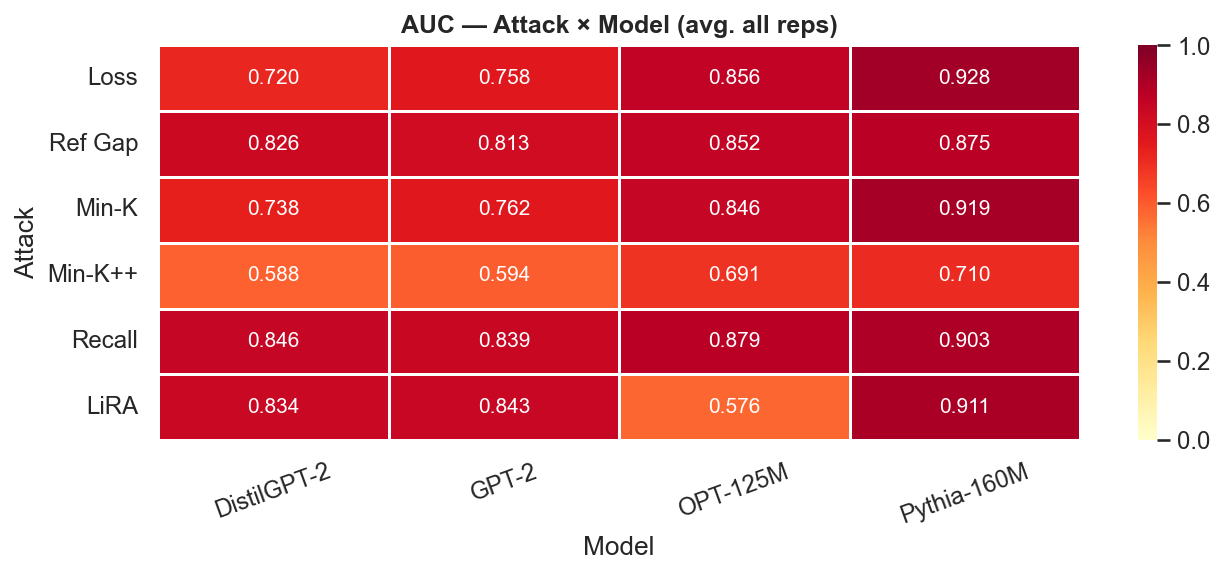
\includegraphics[width=0.48\linewidth]{fig_02_auc_model.png}
\hfill
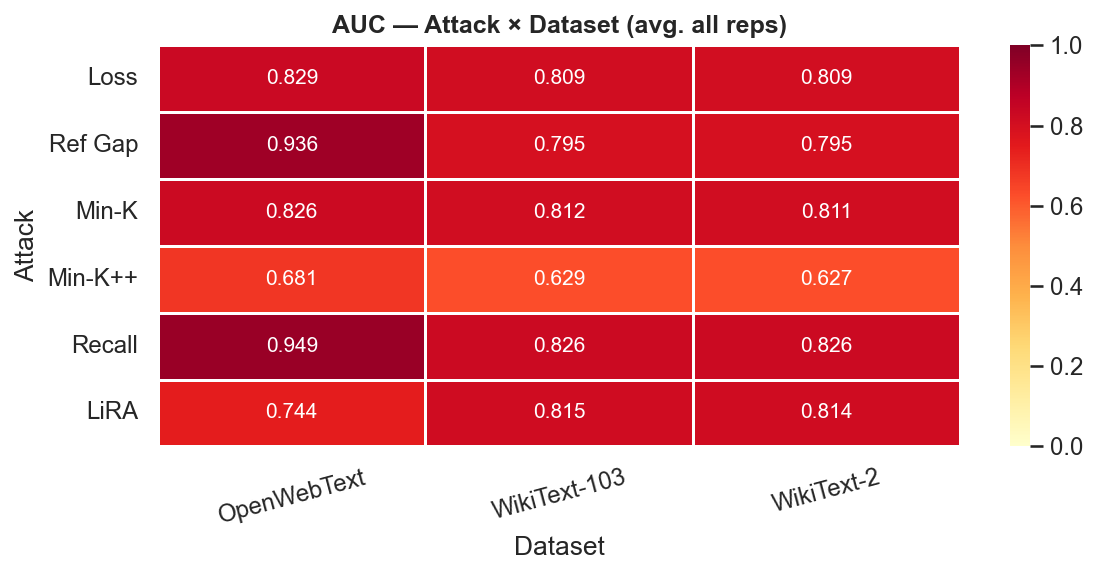
\includegraphics[width=0.48\linewidth]{fig_03_auc_dataset.png}
\caption{\textit{Heatmaps} de AUC por ataque. (Esquerda) Análise por modelo: Pythia-160M exibe a maior vulnerabilidade. (Direita) Análise por \textit{dataset}: OpenWebText produz valores superiores para ataques baseados em referência. Fonte: elaborado pela autora.}
\label{fig:heatmaps_ciarp}
\end{figure}

\subsection{Análise por \textit{Dataset}}

A Tabela~\ref{tab:dataset_ciarp} reporta a AUC por \textit{dataset} e ataque. O OpenWebText produziu os maiores valores de AUC para ataques baseados em referência (0,949 com ReCaLL), enquanto WikiText-2 e WikiText-103 apresentaram resultados praticamente idênticos, confirmando que o domínio do corpus tem maior impacto na vulnerabilidade do que o tamanho do corpus sob condições fixas de \textit{fine-tuning}.

\begin{table}[H]
\centering
\caption{AUC média por \textit{dataset} e ataque.}
\label{tab:dataset_ciarp}
\begin{tabular}{lcccccc}
\toprule
\textbf{\textit{Dataset}} & \textbf{\textit{Loss}} & \textbf{\textit{Ref}} & \textbf{MK} & \textbf{MK++} & \textbf{ReC} & \textbf{LiRA} \\
\midrule
WikiText-2   & 0,809 & 0,795 & 0,811 & 0,627 & 0,826 & 0,814 \\
WikiText-103 & 0,809 & 0,795 & 0,812 & 0,629 & 0,826 & 0,815 \\
OpenWebText  & 0,829 & 0,936 & 0,826 & 0,681 & 0,949 & 0,744 \\
\bottomrule
\end{tabular}
\end{table}

\subsection{Cobertura e Estabilidade}

A Tabela~\ref{tab:coverage_ciarp} apresenta as métricas de cobertura e estabilidade. Os ataques \textit{Loss} e Min-K\% compartilham valores idênticos de AUC (0,816), porém identificam subconjuntos distintos de amostras de treinamento, demonstrando que ataques com desempenho discriminativo semelhante podem expor padrões de vulnerabilidade diferentes.

\begin{table}[H]
\centering
\caption{Cobertura e estabilidade médias nas 48 configurações experimentais.}
\label{tab:coverage_ciarp}
\begin{tabular}{lccc}
\toprule
\textbf{Ataque} & \textbf{Cob. Membros} & \textbf{Cob. \textit{Canaries}} & \textbf{Estabilidade} \\
\midrule
\textit{Loss}       & 0,759 & 1,000 & 1,000 \\
\textit{Ref-gap}    & 0,775 & 1,000 & 1,000 \\
Min-K\%    & 0,764 & 0,998 & 0,898 \\
Min-K\%++  & 0,621 & 0,721 & 1,000 \\
ReCaLL     & 0,796 & 1,000 & 1,000 \\
LiRA       & 0,711 & 1,000 & 1,000 \\
\bottomrule
\end{tabular}
\end{table}

\begin{figure}[H]
    \centering
    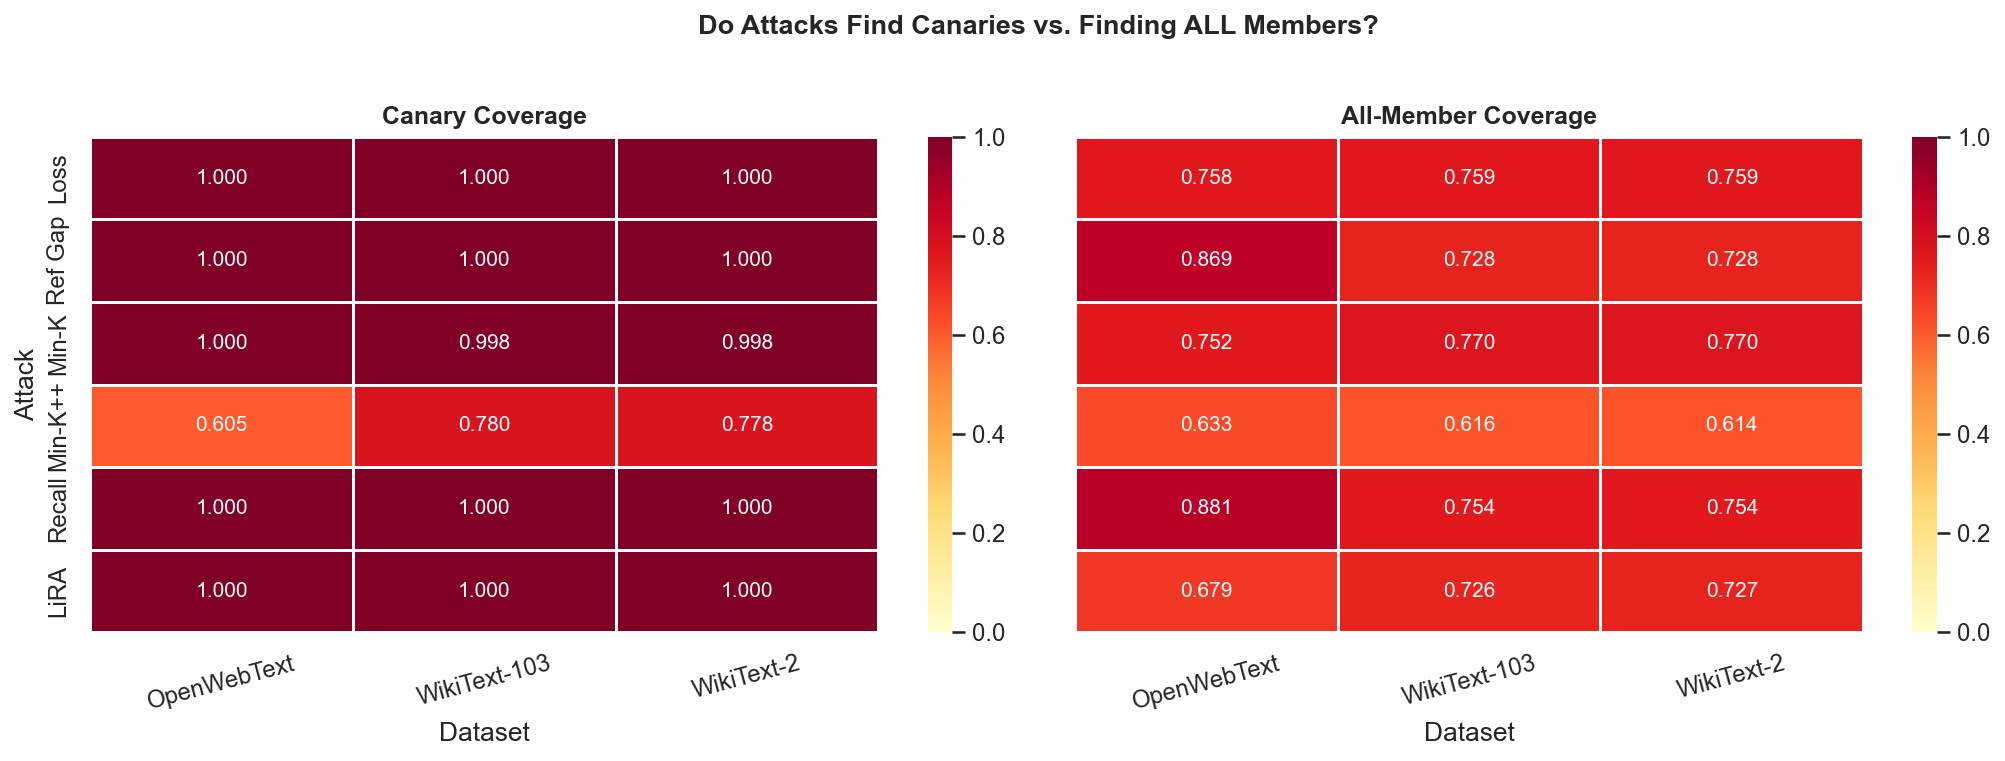
\includegraphics[width=0.85\linewidth]{fig_06_coverage.png}
    \caption{Cobertura de \textit{canaries} versus cobertura de membros. Cinco ataques alcançam cobertura de \textit{canaries} próxima à perfeição; a cobertura de membros é consistentemente inferior. Fonte: elaborado pela autora.}
    \label{fig:coverage_ciarp}
\end{figure}

\begin{figure}[H]
    \centering
    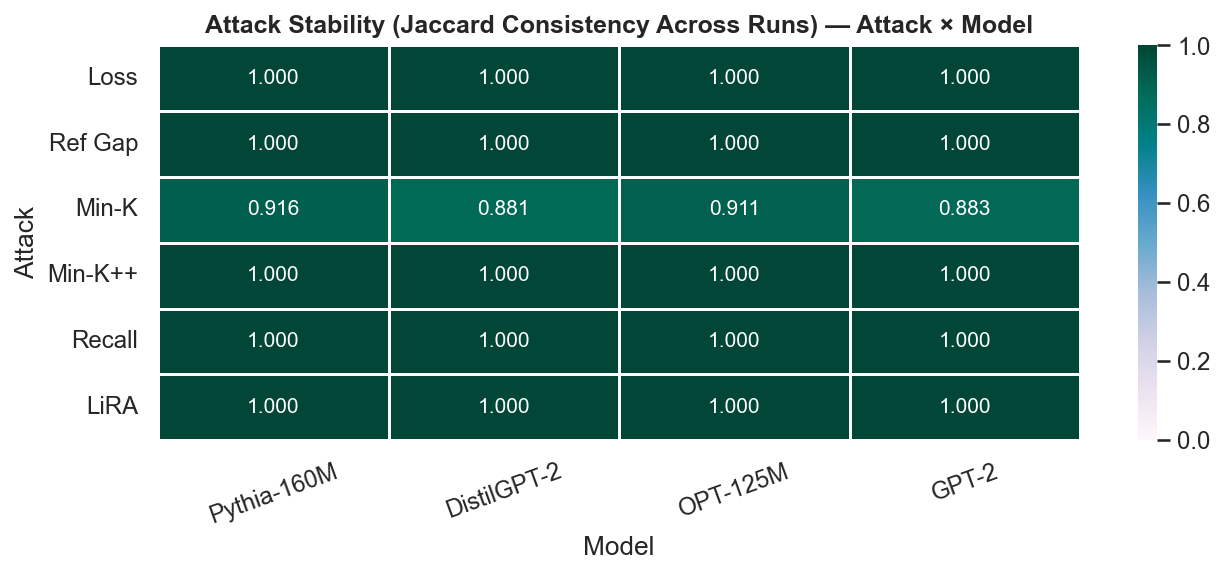
\includegraphics[width=0.85\linewidth]{fig_07_stability.png}
    \caption{Estabilidade (similaridade de Jaccard) por ataque e \textit{dataset}. Ataques determinísticos alcançam estabilidade perfeita; Min-K\% apresenta leve variação devido a perturbações estocásticas. Fonte: elaborado pela autora.}
    \label{fig:stability_ciarp}
\end{figure}

\subsection{Perfis Multidimensionais}

A Figura~\ref{fig:radar_ciarp} apresenta os perfis radar de comportamento dos ataques por \textit{dataset}, sintetizando múltiplas dimensões de auditoria simultaneamente. O ReCaLL e o \textit{reference-gap} exibem os perfis mais consistentes, enquanto o Min-K\%++ mostra comportamento sistematicamente mais fraco em todas as dimensões avaliadas.

\begin{figure}[H]
    \centering
    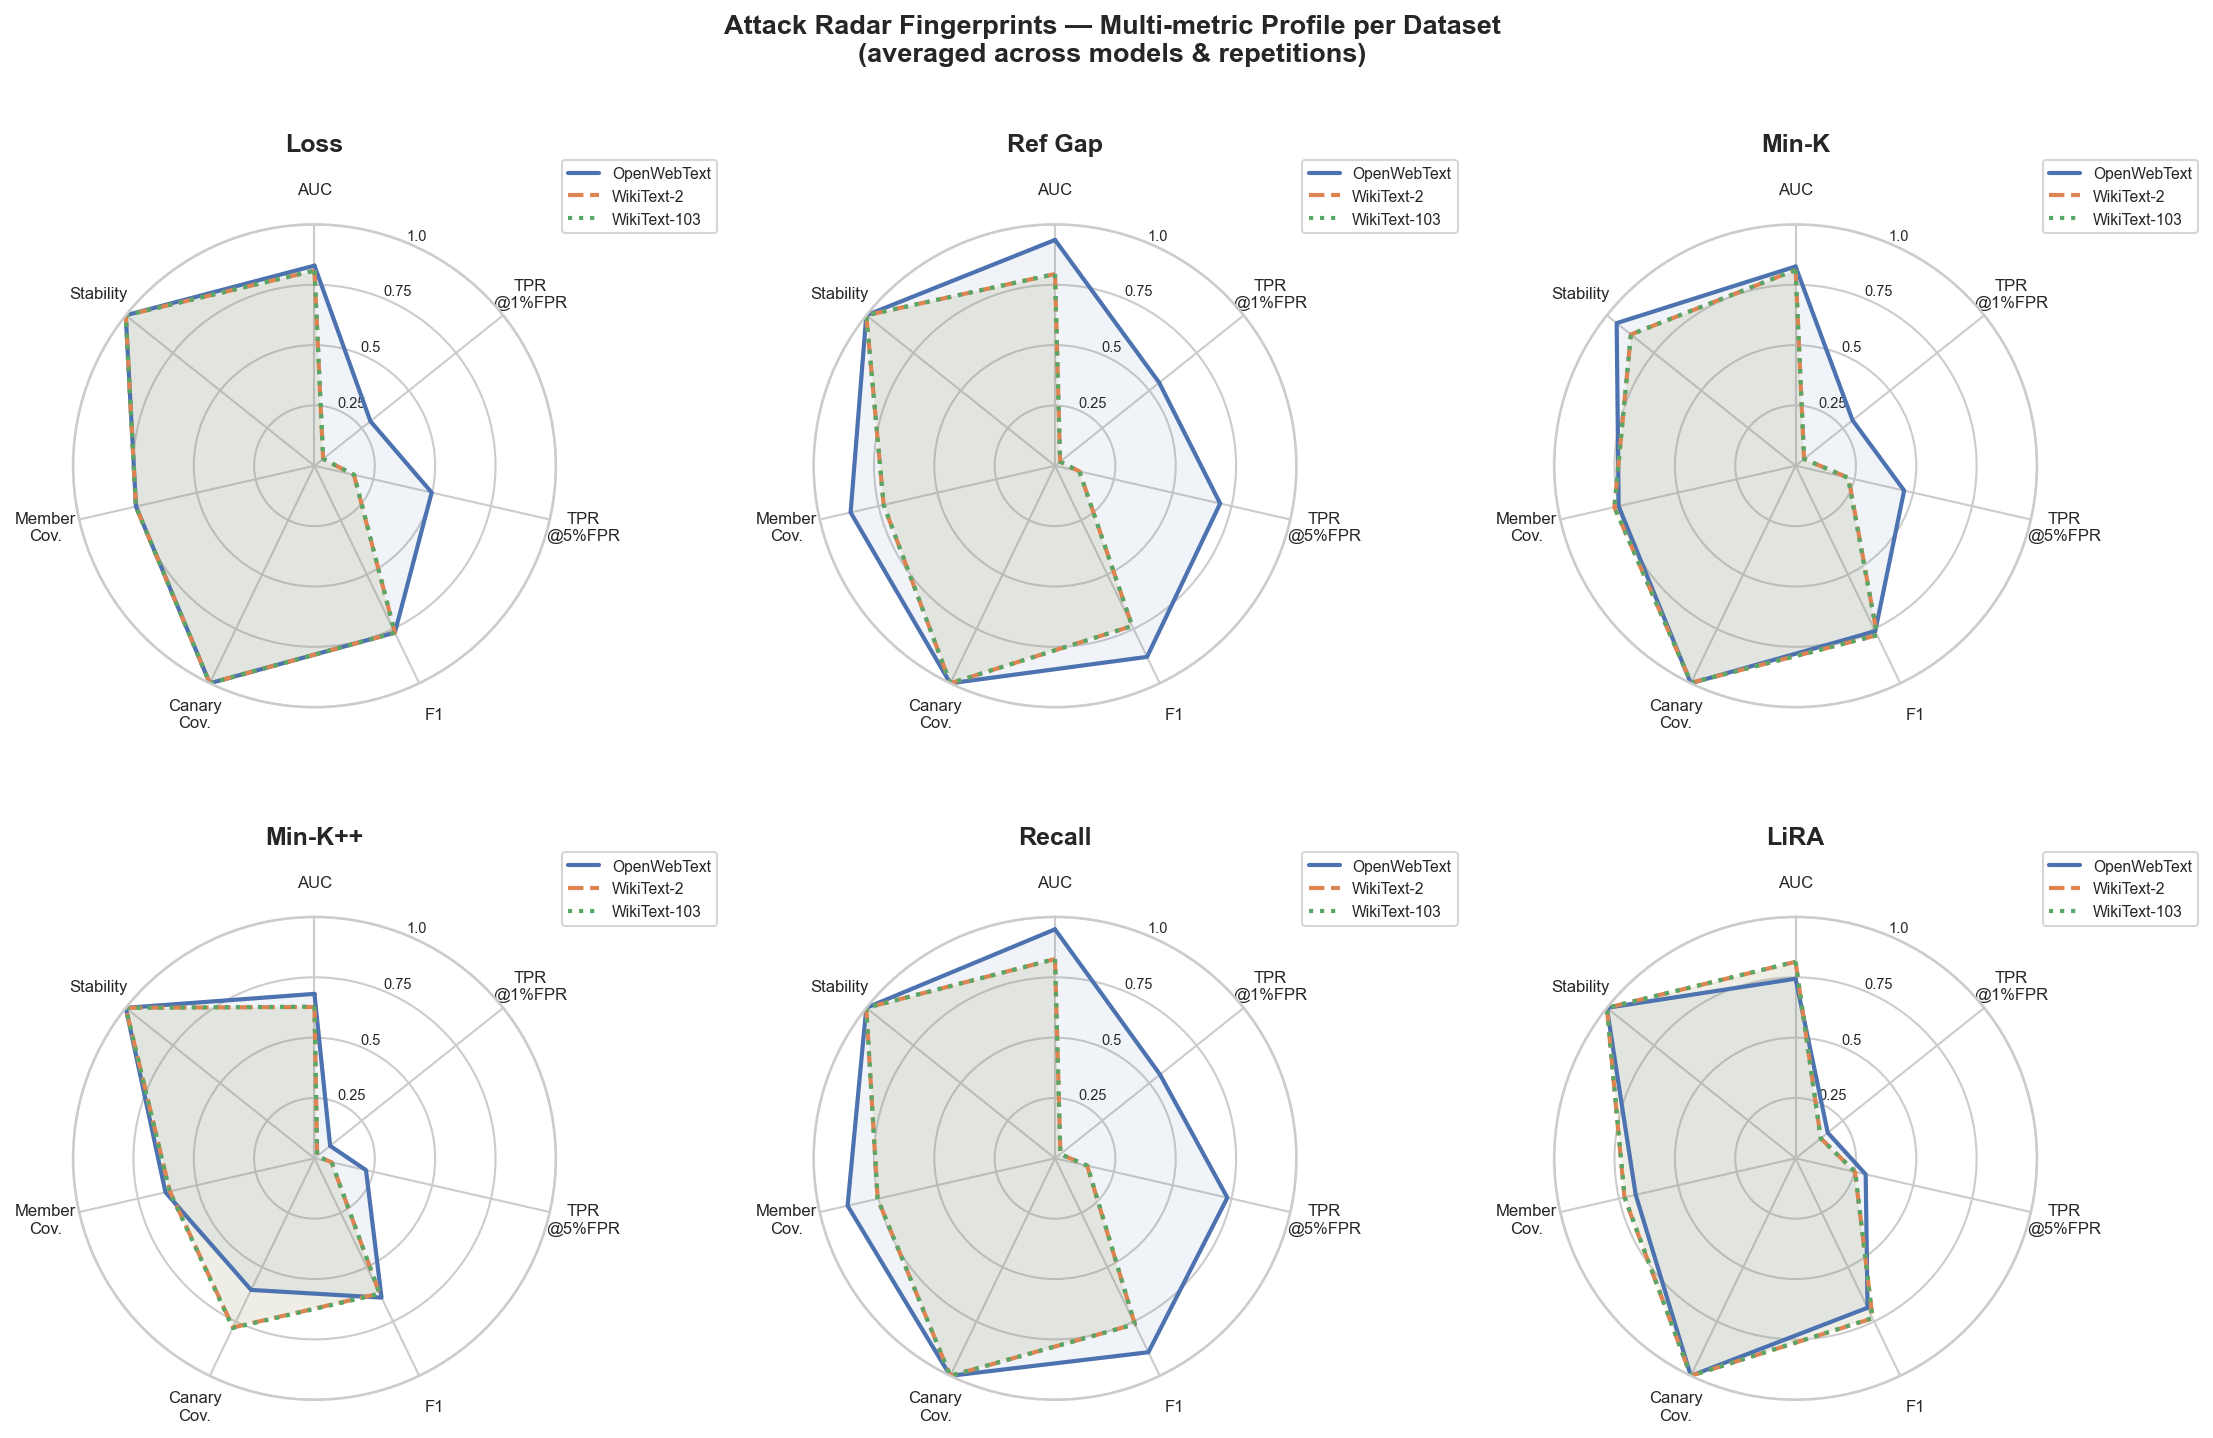
\includegraphics[width=0.85\linewidth]{fig_38_radar.png}
    \caption{Perfis radar do comportamento dos ataques por \textit{dataset}. Cada polígono sintetiza múltiplas dimensões de auditoria, incluindo AUC, F1, detecção em baixo FPR, cobertura e estabilidade. Fonte: elaborado pela autora.}
    \label{fig:radar_ciarp}
\end{figure}

\begin{figure}[H]
    \centering
    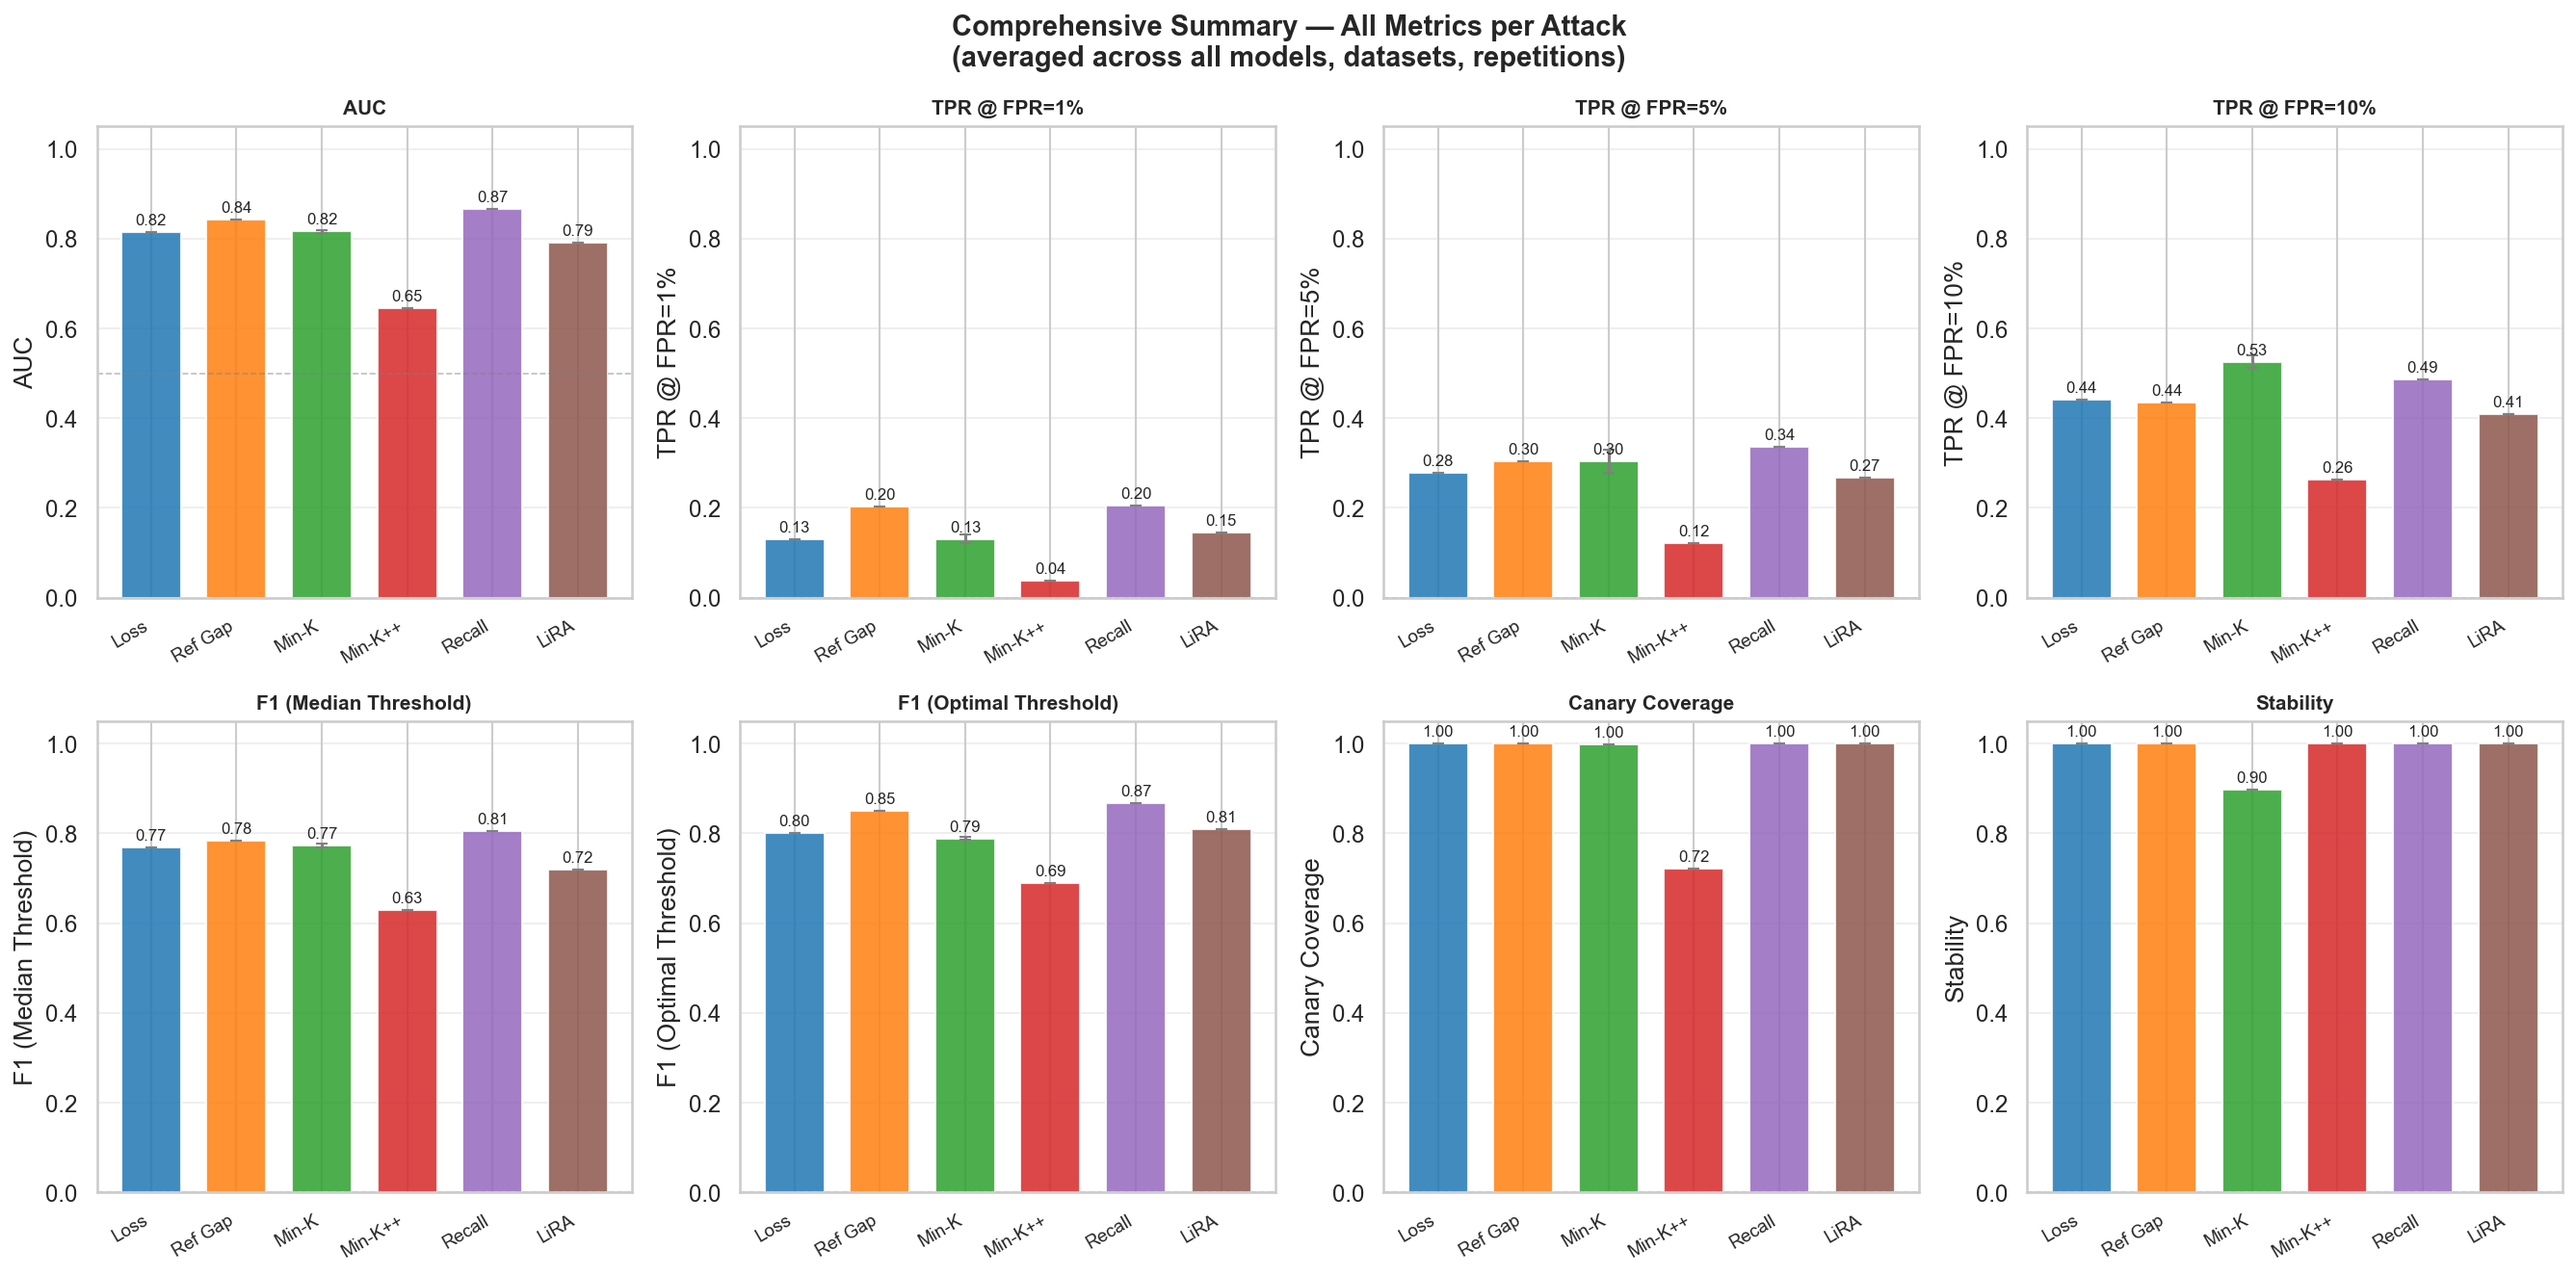
\includegraphics[width=0.85\linewidth]{fig_40_comprehensive.png}
    \caption{Comparação abrangente das métricas de auditoria entre ataques. ReCaLL alcança o melhor desempenho geral, enquanto Min-K\%++ apresenta resultados consistentemente inferiores em múltiplas dimensões de avaliação. Fonte: elaborado pela autora.}
    \label{fig:comprehensive_ciarp}
\end{figure}

\section{Discussão e Implicações para Fed-IDS}

Os resultados experimentais indicam que a vulnerabilidade de pertencimento é fortemente influenciada pela interação entre arquitetura do modelo, domínio do \textit{dataset} e estratégia de ataque. O Pythia-160M consistentemente exibiu a maior suscetibilidade, enquanto o domínio do corpus (OpenWebText versus WikiText) demonstrou impacto maior na vulnerabilidade do que o tamanho do corpus isoladamente.

Do ponto de vista metodológico, os achados demonstram que a AUC agregada isoladamente é insuficiente para auditoria de privacidade, uma vez que ataques com desempenho discriminativo semelhante podem detectar subconjuntos distintos de amostras vulneráveis. Dimensões complementares como cobertura, estabilidade e análise por amostra proporcionam uma caracterização substancialmente mais informativa do vazamento de pertencimento.

Esses resultados possuem implicações diretas para a auditoria de Fed-IDS proposta nesta dissertação:

\begin{enumerate}[label=(\roman*)]
    \item A abordagem multidimensional será transposta para o contexto federado, avaliando como diferentes algoritmos de agregação (FedAvg, FedProx, SCAFFOLD, FedOpt) influenciam a vulnerabilidade a MIA em sistemas de detecção de intrusões.
    \item A análise de cobertura e estabilidade será aplicada para verificar se ataques que funcionam bem em cenários centralizados mantêm eficácia em configurações federadas com dados heterogêneos (\textit{non-IID}).
    \item As defesas híbridas (DP-SGD, \textit{AdaMixup}, compressão de gradientes) serão avaliadas utilizando as cinco dimensões do arcabouço proposto, permitindo quantificar o \textit{trade-off} entre privacidade, utilidade e custo computacional em Fed-IDS.
\end{enumerate}

A validação do arcabouço em modelos de linguagem fornece evidências de sua aplicabilidade e robustez, constituindo a base metodológica para a extensão ao cenário federado de detecção de intrusões.


\section{Conclusões Parciais}
\label{sec:conclusoes}

Este trabalho realizou uma revisão sistemática e analítica sobre o estado da arte em segurança e privacidade aplicadas ao Fed-IDS, com ênfase na detecção e mitigação de MIA. A investigação permitiu identificar padrões, lacunas e tendências que moldam o atual panorama da pesquisa em aprendizado federado voltado à cibersegurança.

Entre os principais achados, observou-se que a literatura converge para três frentes complementares: (i) aprimoramento da privacidade via mecanismos de ruído e regularização (como DP-SGD e \textit{dropout} diferencial); (ii) uso crescente de estratégias híbridas, que combinam defesas complementares em múltiplos níveis; e (iii) carência de padronização tanto em \textit{benchmarks} quanto em métricas de avaliação da privacidade. Essa ausência de uniformização metodológica dificulta a reprodutibilidade dos resultados e impede comparações precisas entre diferentes abordagens.

Como contribuição teórica, este estudo sistematizou as evidências e delineou um \textit{framework} conceitual de auditoria e mitigação em Fed-IDS, representado na Figura~\ref{fig:pipeline_fedids}. O modelo propõe a integração entre auditoria adversarial (via ataques LiRA e variantes), defesas híbridas (DP-SGD, \textit{AdaMixup} e compressão de gradientes) e análise empírica do \textit{trade-off} entre privacidade e utilidade, constituindo uma base metodológica sólida para futuras implementações experimentais.

Adicionalmente, a validação do arcabouço de auditoria multidimensional em modelos de linguagem (Capítulo~\ref{sec:auditoria_llm}) demonstrou a viabilidade e a robustez da abordagem proposta, com resultados publicados no CIARP 2026. Esse trabalho evidenciou que a AUC agregada é insuficiente para caracterizar riscos de privacidade, motivando a adoção de dimensões complementares como cobertura, estabilidade e vulnerabilidade por amostra.

Do ponto de vista prático, a revisão reforça a urgência de estabelecer \textit{benchmarks} públicos e métricas padronizadas de privacidade para sistemas federados de detecção de intrusões. Tal padronização é essencial para a maturidade científica do campo e para o avanço de sistemas auditáveis e confiáveis em ambientes distribuídos.

\section{Próximos Passos}

As etapas subsequentes desta pesquisa compreendem:

\begin{enumerate}[label=(\roman*)]
    \item Transposição do arcabouço de auditoria multidimensional para o cenário federado, com implementação de \textit{baseline} Fed-IDS utilizando FedAvg, FedProx, SCAFFOLD e FedOpt sobre \textit{datasets} de detecção de intrusões (CIC-IDS2017, UNSW-NB15).
    \item Implementação e avaliação dos seis ataques de inferência de pertencimento no contexto federado, analisando o impacto da heterogeneidade de dados (\textit{non-IID}) e do número de clientes.
    \item Integração e avaliação de defesas híbridas (DP-SGD combinado com regularização e compressão de gradientes), quantificando o \textit{trade-off} entre privacidade, utilidade e custo computacional.
    \item Análise comparativa dos resultados e redação final da dissertação.
\end{enumerate}

\section{Cronograma}
\label{sec:cronograma_tab}

O presente cronograma descreve as atividades planejadas entre dezembro de 2025, logo após a entrega inicial desta etapa, até novembro de 2026. Nesse intervalo, a qualificação está prevista para julho de 2026 e a defesa da dissertação para novembro de 2026. As tarefas foram organizadas de modo a alinhar a fundamentação teórica e os trabalhos correlatos discutidos nas seções anteriores com a implementação experimental, a auditoria de ataques e a análise crítica dos resultados.  

\begin{table}[H]
\centering
\scriptsize
\caption{Cronograma de atividades  dezembro/2025 a novembro/2026.}
\label{tab:cronograma}
\renewcommand{\arraystretch}{1.3}
\begin{tabularx}{\linewidth}{|p{4.2cm}|*{12}{>{\centering\arraybackslash}X|}}
\hline
\textbf{Atividade} 
& \rotatebox{90}{Dez/25} & \rotatebox{90}{Jan/26} & \rotatebox{90}{Fev/26} 
& \rotatebox{90}{Mar/26} & \rotatebox{90}{Abr/26} & \rotatebox{90}{Mai/26} 
& \rotatebox{90}{Jun/26} & \rotatebox{90}{Jul/26} & \rotatebox{90}{Ago/26} 
& \rotatebox{90}{Set/26} & \rotatebox{90}{Out/26} & \rotatebox{90}{Nov/26} \\ \hline

Revisão da fundamentação teórica & X & X &   &   &   &   &   &   &   &   &   &   \\ \hline
Levantamento e preparação de datasets & X & X & X &   &   &   &   &   &   &   &   &   \\ \hline
Implementação de baseline Fed-IDS &   &   &   & X & X &   &   &   &   &   &   &   \\ \hline
Implementação de ataques MIA &   &   &   &   & X & X &   &   &   &   &   &   \\ \hline
Experimentos preliminares e coleta de métricas &   &   &   &   &   & X & X &   &   &   &   &   \\ \hline
Redação parcial e ajustes para qualificação &   &   &   &   &   & X & X &   &   &   &   &   \\ \hline
Qualificação &   &   &   &   &   &   &   & X &   &   &   &   \\ \hline
Integração de defesas híbridas &   &   &   &   &   &   &   &   & X & X &   &   \\ \hline
Execução de experimentos finais e análise crítica &   &   &   &   &   &   &   &   & X & X & X &   \\ \hline
Redação final da dissertação &   &   &   &   &   &   &   &   &   & X & X &   \\ \hline
Revisão final e preparação para defesa &   &   &   &   &   &   &   &   &   &   & X &   \\ \hline
Defesa de mestrado &   &   &   &   &   &   &   &   &   &   &   & X \\ \hline

\end{tabularx}
\end{table}

O cronograma demonstra a progressão lógica da pesquisa: primeiro consolida-se a base teórica e a infraestrutura experimental; em seguida, são conduzidas implementações de algoritmos e ataques; por fim, as defesas híbridas são avaliadas sob métricas rigorosas. Essa sequência garante alinhamento entre os objetivos da dissertação e as lacunas de pesquisa destacadas na seção~\ref{sec:discussoes_aberto}.



% --------------------------------------------------------
% ELEMENTOS PÓS-TEXTUAIS
% --------------------------------------------------------

\postextual


% --------------------------------------------------------
% REFERÊNCIAS BIBLIOGRÁFICAS
% --------------------------------------------------------

\bibliography{referencias}


% --------------------------------------------------------
% GLOSSÁRIO
% --------------------------------------------------------

% Consulte o manual da classe abntex2 para orientações sobre o glossário.
%\glossary


% --------------------------------------------------------
% APÊNDICES
% --------------------------------------------------------

% Inicia os apêndices
%\begin{apendicesenv}
% Imprime uma página indicando o início dos apêndices
%\partapendices
% Criação do apêndice
%\end{apendicesenv}


% --------------------------------------------------------
% ÍNDICE REMISSIVO
% --------------------------------------------------------

\printindex


% --------------------------------------------------------
% FINAL DO DOCUMENTO
% --------------------------------------------------------

\end{document}
